% Options for packages loaded elsewhere
\PassOptionsToPackage{unicode}{hyperref}
\PassOptionsToPackage{hyphens}{url}
\PassOptionsToPackage{dvipsnames,svgnames,x11names}{xcolor}
%
\documentclass[
  10,
  letterpaper,
  DIV=11,
  numbers=noendperiod]{scrreport}

\usepackage{amsmath,amssymb}
\usepackage{iftex}
\ifPDFTeX
  \usepackage[T1]{fontenc}
  \usepackage[utf8]{inputenc}
  \usepackage{textcomp} % provide euro and other symbols
\else % if luatex or xetex
  \usepackage{unicode-math}
  \defaultfontfeatures{Scale=MatchLowercase}
  \defaultfontfeatures[\rmfamily]{Ligatures=TeX,Scale=1}
\fi
\usepackage{lmodern}
\ifPDFTeX\else  
    % xetex/luatex font selection
\fi
% Use upquote if available, for straight quotes in verbatim environments
\IfFileExists{upquote.sty}{\usepackage{upquote}}{}
\IfFileExists{microtype.sty}{% use microtype if available
  \usepackage[]{microtype}
  \UseMicrotypeSet[protrusion]{basicmath} % disable protrusion for tt fonts
}{}
\makeatletter
\@ifundefined{KOMAClassName}{% if non-KOMA class
  \IfFileExists{parskip.sty}{%
    \usepackage{parskip}
  }{% else
    \setlength{\parindent}{0pt}
    \setlength{\parskip}{6pt plus 2pt minus 1pt}}
}{% if KOMA class
  \KOMAoptions{parskip=half}}
\makeatother
\usepackage{xcolor}
\usepackage[lmargin=2cm,rmargin=2cm,tmargin=2cm,bmargin=3cm]{geometry}
\setlength{\emergencystretch}{3em} % prevent overfull lines
\setcounter{secnumdepth}{5}
% Make \paragraph and \subparagraph free-standing
\ifx\paragraph\undefined\else
  \let\oldparagraph\paragraph
  \renewcommand{\paragraph}[1]{\oldparagraph{#1}\mbox{}}
\fi
\ifx\subparagraph\undefined\else
  \let\oldsubparagraph\subparagraph
  \renewcommand{\subparagraph}[1]{\oldsubparagraph{#1}\mbox{}}
\fi


\providecommand{\tightlist}{%
  \setlength{\itemsep}{0pt}\setlength{\parskip}{0pt}}\usepackage{longtable,booktabs,array}
\usepackage{calc} % for calculating minipage widths
% Correct order of tables after \paragraph or \subparagraph
\usepackage{etoolbox}
\makeatletter
\patchcmd\longtable{\par}{\if@noskipsec\mbox{}\fi\par}{}{}
\makeatother
% Allow footnotes in longtable head/foot
\IfFileExists{footnotehyper.sty}{\usepackage{footnotehyper}}{\usepackage{footnote}}
\makesavenoteenv{longtable}
\usepackage{graphicx}
\makeatletter
\def\maxwidth{\ifdim\Gin@nat@width>\linewidth\linewidth\else\Gin@nat@width\fi}
\def\maxheight{\ifdim\Gin@nat@height>\textheight\textheight\else\Gin@nat@height\fi}
\makeatother
% Scale images if necessary, so that they will not overflow the page
% margins by default, and it is still possible to overwrite the defaults
% using explicit options in \includegraphics[width, height, ...]{}
\setkeys{Gin}{width=\maxwidth,height=\maxheight,keepaspectratio}
% Set default figure placement to htbp
\makeatletter
\def\fps@figure{htbp}
\makeatother

\newcommand{\bx}{\mathbf{x}}
\newcommand{\bt}{\boldsymbol{\theta}}
\newcommand{\dkl}{\mathrm{d}_{\mathrm{KL}}}
\newcommand{\dtv}{\mathrm{d}_{\mathrm{TV}}}
\newcommand{\emv}{\hat{\theta}_{\mathrm{emv}}}
\newcommand{\ent}{\mathrm{Ent}}
\usepackage{mathrsfs}
\KOMAoption{captions}{tableheading}
\makeatletter
\makeatother
\makeatletter
\@ifpackageloaded{bookmark}{}{\usepackage{bookmark}}
\makeatother
\makeatletter
\@ifpackageloaded{caption}{}{\usepackage{caption}}
\AtBeginDocument{%
\ifdefined\contentsname
  \renewcommand*\contentsname{Table des matières}
\else
  \newcommand\contentsname{Table des matières}
\fi
\ifdefined\listfigurename
  \renewcommand*\listfigurename{Liste des Figures}
\else
  \newcommand\listfigurename{Liste des Figures}
\fi
\ifdefined\listtablename
  \renewcommand*\listtablename{Liste des Tables}
\else
  \newcommand\listtablename{Liste des Tables}
\fi
\ifdefined\figurename
  \renewcommand*\figurename{Figure}
\else
  \newcommand\figurename{Figure}
\fi
\ifdefined\tablename
  \renewcommand*\tablename{Table}
\else
  \newcommand\tablename{Table}
\fi
}
\@ifpackageloaded{float}{}{\usepackage{float}}
\floatstyle{ruled}
\@ifundefined{c@chapter}{\newfloat{codelisting}{h}{lop}}{\newfloat{codelisting}{h}{lop}[chapter]}
\floatname{codelisting}{Listing}
\newcommand*\listoflistings{\listof{codelisting}{Liste des Listings}}
\usepackage{amsthm}
\theoremstyle{plain}
\newtheorem{theorem}{Théorème}[chapter]
\theoremstyle{definition}
\newtheorem{exercise}{Exercice}[chapter]
\theoremstyle{plain}
\newtheorem{proposition}{Proposition}[chapter]
\theoremstyle{definition}
\newtheorem{definition}{Définition}[chapter]
\theoremstyle{definition}
\newtheorem{example}{Exemple}[chapter]
\theoremstyle{plain}
\newtheorem{lemma}{Lemme}[chapter]
\theoremstyle{remark}
\AtBeginDocument{\renewcommand*{\proofname}{Preuve}}
\newtheorem*{remark}{Remarque}
\newtheorem*{solution}{Solution}
\makeatother
\makeatletter
\@ifpackageloaded{caption}{}{\usepackage{caption}}
\@ifpackageloaded{subcaption}{}{\usepackage{subcaption}}
\makeatother
\makeatletter
\@ifpackageloaded{tcolorbox}{}{\usepackage[skins,breakable]{tcolorbox}}
\makeatother
\makeatletter
\@ifundefined{shadecolor}{\definecolor{shadecolor}{rgb}{.97, .97, .97}}
\makeatother
\makeatletter
\makeatother
\makeatletter
\makeatother
\ifLuaTeX
\usepackage[bidi=basic]{babel}
\else
\usepackage[bidi=default]{babel}
\fi
\babelprovide[main,import]{french}
% get rid of language-specific shorthands (see #6817):
\let\LanguageShortHands\languageshorthands
\def\languageshorthands#1{}
\ifLuaTeX
  \usepackage{selnolig}  % disable illegal ligatures
\fi
\IfFileExists{bookmark.sty}{\usepackage{bookmark}}{\usepackage{hyperref}}
\IfFileExists{xurl.sty}{\usepackage{xurl}}{} % add URL line breaks if available
\urlstyle{same} % disable monospaced font for URLs
\hypersetup{
  pdftitle={Statistiques Fondamentales},
  pdfauthor={Simon Coste},
  pdflang={fr},
  colorlinks=true,
  linkcolor={blue},
  filecolor={Maroon},
  citecolor={Blue},
  urlcolor={Blue},
  pdfcreator={LaTeX via pandoc}}

\title{Statistiques Fondamentales}
\author{Simon Coste}
\date{2025-01-08}

\begin{document}
\maketitle
\ifdefined\Shaded\renewenvironment{Shaded}{\begin{tcolorbox}[borderline west={3pt}{0pt}{shadecolor}, boxrule=0pt, frame hidden, breakable, interior hidden, enhanced, sharp corners]}{\end{tcolorbox}}\fi

\renewcommand*\contentsname{Table des matières}
{
\hypersetup{linkcolor=}
\setcounter{tocdepth}{2}
\tableofcontents
}
\bookmarksetup{startatroot}

\hypertarget{organisation}{%
\chapter*{Organisation}\label{organisation}}
\addcontentsline{toc}{chapter}{Organisation}

\markboth{Organisation}{Organisation}

Bienvenue sur la page du cours de Statistiques Fondamentales (STF8) du
master Mathématiques Fondamentales et Appliquées de l'Université
Paris-Cité. Les notes de cours sont accessibles à tous. De nombreux
auteurs s'y sont succédés ; je suis le dernier en date, mais les
versions précédentes ont été travaillées par Clément Levrard, Stéphane
Boucheron, Stéphane Gaïffas, Pierre Youssef.

Le cours reprendra l'année prochaine, en janvier 2025.

\begin{itemize}
\tightlist
\item
  \textbf{Calcul de la note finale}. Trois quantités entrent en jeu :~la
  note de contrôle continu \(c \in [0,10]\), la note du partiel
  \(p\in [0,20]\), et la note que vous obtiendrez à l'examen,
  \(e \in [0,20]\). La note finale \(f \in [0,20]\) est donnée par la
  formule
  \[ f = 20^{\theta} \left(\frac{\max\{p,e\} + e}{2}\right)^{1 - \theta} \]
  où \(\theta = 0.3 \times c/10\). C'est une moyenne géométrique qui ne
  pénalise personne, et qui ne peut que tirer votre note vers le haut si
  vous avez une note de contrôle continu \(c\) strictement positive.
\end{itemize}

\hypertarget{utiliser-ce-site}{%
\section*{Utiliser ce site}\label{utiliser-ce-site}}
\addcontentsline{toc}{section}{Utiliser ce site}

\markright{Utiliser ce site}

Chaque chapitre de ce livre contient une page dédiée au cours théorique,
et contiendra dans un futur proche une page d'exercices.

Ces notes sont mises en lignes et totalement accessibles via
\href{https://quarto.org}{Quarto}. Si vous savez comment utiliser
\texttt{git}, n'hésitez pas à corriger toutes les erreurs que vous
pourriez voir (et Dieu sait qu'elles seront nombreuses) via des pull
requests.

\bookmarksetup{startatroot}

\hypertarget{introduction}{%
\chapter{Introduction}\label{introduction}}

Les outils des statistiques furent créés pour analyser des phénomènes
quantitatifs dans lesquels la présence de \emph{bruit} ou de
\emph{hasard} rendait l'analyse classique moins opérante. Il peut
typiquement s'agir de problèmes dans lesquels de nombreuses données
indépendantes ont été générées par le même phénomène. Dans cette
section, nous allons développer un exemple pour bien comprendre les
questions qui se posent et la façon de les résoudre, puis nous poserons
quelques bases qui nous permettront d'utiliser le langage des
mathématiques.

\hypertarget{un-exemple-pour-fixer-les-iduxe9es}{%
\section{Un exemple pour fixer les
idées}\label{un-exemple-pour-fixer-les-iduxe9es}}

Une grande enseigne de distribution possède \(n=100\) magasins
identiques, qui génèrent chaque année un chiffre d'affaire annuel (CA,
en millions d'euros). Ce chiffre oscille autour d'une valeur de
référence \(\mu\). Cette valeur n'est pas observée ; ce qui est observé,
ce sont tous les chiffres d'affaires des \(n\) magasins, qui fluctuent
tous autour de la vraie valeur \(\mu\). Ces fluctuations proviennent de
nombreuses sources : erreurs comptables, perturbations des ventes dues
aux fournisseurs ou aux prix, etc. Ce qu'on observe, c'est donc des
chiffres \(x_1, \dotsc, x_n\) qui ne sont pas tous égaux ; comment avoir
une idée de la véritable valeur de \(\mu\) ?

\textbf{Estimation.} Évidemment, la moyenne empirique
\[\bar x_n = \frac{x_1+\dotsb + x_n}{n}\] vient naturellement à
l'esprit. En faisant le calcul, on trouve \(\bar{x}_n \approx 21,6\).
Cette valeur est une \emph{estimation} du CA moyen \(\mu\). Ce chiffre
peut être utilisé par l'enseigne, par exemple pour jauger la rentabilité
d'un possible plan d'ouverture de nouveaux magasins.

\textbf{Précision}. On pourrait se demander à quel point cette
estimation est précise ou, disons, essayer de quantifier l'erreur
possible qu'on fait si l'on dit que \(\mu\) est égal à 21,6 millions
d'euros. Cela nécessite de faire quelques hypothèses sur le hasard qui
génère les fluctuations des \(x_i\) autour de \(\mu\). Ces fluctuations
observées au cours de l'année proviennent de l'agrégation de toutes les
fluctuations quotidiennes, lesquelles sont à peu près indépendantes, et
pour cette raison on peut supposer (pour commencer) que ces fluctuations
sont gaussiennes et ont à peu près la même variance, disons
\(\sigma^2=1\). Comme on a supposé que les \(x_i\) sont des réalisations
d'une loi gaussienne \(N(\mu, 1)\), alors on sait que \(\bar{x}_n\) est
la réalisation d'une loi \(N(\mu, 1/n)\), ou encore que
\(\bar{x}_n - \mu\) est la réalisation d'une gaussienne centrée de
variance \(1/n\). Les lois gaussiennes sont bien connues ; par exemple,
avec probabilité supérieure à 99\%, une gaussienne \(N(0, \sigma^2)\)
est comprise entre les valeurs \(-2,96\sigma\) et \(2,96\sigma\).
Autrement dit, il y a 99\% de chances pour que le nombre
\(|\bar{x}-\mu|\), qui représente l'erreur d'estimation, soit plus
petite que \(2,96/\sqrt{n} = 2,96/10 \approx 0,3\).

Ce dernier raisonnement peut être vu d'une autre façon. Dire que
\(\bar{x}_n\) et \(\mu\) ne diffèrent pas de plus de \(0,3\), c'est
équivalent à dire que \(\mu\) appartient à l'intervalle
\([\bar{x} - 0,3, \bar{x} +0,3]\). En d'autres termes, avec une
probabilité supérieure à 99\%, le vrai CA \(\mu\) de chaque magasin se
situe entre \(21,3\) et \(21,9\). Cela laisse tout de même une chance de
1\% que le paramètre \(\mu\) ne soit pas dans cette région.

\textbf{Tests}. Il existe encore un autre point de vue sur ce problème.
Par exemple, le conseil d'administration de la firme veut s'assurer que
le dirigeant a bien tenu sa promesse selon laquelle le CA de chaque
magasin était supérieur à 21 millions d'euros. La valeur exacte de
\(\mu\) n'est pas le plus important : ce qui nous intéresse maintenant,
c'est plutôt d'être sûrs que \(\mu\) n'est pas inférieur au seuil de 21.
Le dirigeant, fin statisticien, effectue alors un raisonnement par
l'absurde \emph{en probabilité}. Supposons que le CA \(\mu\) soit
effectivement égal à 21 (ou même, inférieur). Alors, par les mêmes
calculs que ci-dessus, cela voudrait dire qu'avec 99\% de chances,
\(\bar{x}_n\) et \(21\) ne devraient pas différer de plus de \(0,3\) ;
autrement dit, que \(\bar{x}_n\) devrait se situer entre \(20,7\) et
\(21,3\). Ce n'est pas le cas, puisque \(\bar{x}_n = 21,6\). Si \(\mu\)
est réellement plus petit que 21, alors ce qu'on a observé est
extrêmement peu probable. Par contraposée probabiliste, il est
raisonnable de rejeter l'hypothèse selon laquelle \(\mu\) est inférieur
à 21.

\begin{center}\rule{0.5\linewidth}{0.5pt}\end{center}

Les trois points de vue donnés ci-dessus sont en quelque sorte les
piliers de l'analyse statistique. L'estimation consiste à deviner une
valeur cachée dans du bruit ; les intervalles de confiance consistent à
donner une région dans laquelle se trouve cette valeur ; les tests
d'hypothèse permettent de raisonner de façon logique sur cette valeur.

L'objectif du cours de statistiques de quantifier l'incertitude liée au
hasard dans chacun de ces objectifs. Comme dans les exemples donnés
ci-dessus, c'est un ensemble de méthodes scientifiques qui s'appuient
sur la théorie des probabilités ; dans ce cours, on fera des
\emph{hypothèses} sur le hasard qui est en jeu, et on en tirera des
conséquences \emph{probables} sur le modèle sous-jacent. En théorie des
probabilités, le jeu est plutôt inverse : partant d'un modèle
probabiliste fixé, on essaie de déterminer quel sera le comportement des
réalisations de ce modèle. Il semble difficile de faire l'un sans
l'autre.

\hypertarget{quest-ce-quun-probluxe8me-statistique}{%
\section{Qu'est-ce qu'un problème statistique
?}\label{quest-ce-quun-probluxe8me-statistique}}

Il n'y aurait pas de statistiques s'il n'y avait pas de monde réel, et
comme chacun sait, le monde réel est principalement composé de quantités
aléatoires.

Un problème statistique tire donc toujours sa source d'un ensemble
d'observations, disons \(n\) observations notées \(x_1, \dotsc, x_n\)
;~cet ensemble d'observations est appelé un \emph{échantillon}.
L'hypothèse de base de tout travail statistique consiste à supposer que
cet échantillon suit une certaine loi de probabilité ; l'objectif est de
trouver laquelle. Évidemment, on ne va pas partir de rien : il faut bien
faire des hypothèse minimales sur cette loi. Ce qu'on appelle un
\emph{modèle statistique} est le choix d'une famille de lois de
probabilités que l'on suppose pertinentes.

\begin{definition}[]\protect\hypertarget{def-mst}{}\label{def-mst}

Formellement, choisir un modèle statistique revient à choisir trois
choses :~

\begin{itemize}
\tightlist
\item
  \(\mathcal{X}\), l'espace dans lequel vit notre échantillon ;~
\item
  \(\mathscr{F}\), une tribu sur \(\mathcal{X}\), pour donner du sens à
  ce qui est observable ou non ;
\item
  \((P_\theta)_{\theta \in \Theta}\), une famille de mesures de
  probabilités sur \(\mathcal{X}\) indexée par \(\theta \in \Theta\), où
  \(\Theta\) est appelé espace des paramètres. On écrira fréquemment
  \(\mathbb{E}_\theta\) ou \(\mathrm{Var}_\theta\) pour désigner des
  espérances, variances, etc., calculées avec la loi \(P_\theta\).
\end{itemize}

\end{definition}

En pratique, dans ce cours, on aura toujours un échantillon
\((x_1, \dotsc, x_n)\) où les \(x_i\) vivent dans un même espace, disons
\(\mathbb{R}^d\) pour simplifier. On devrait donc écrire
\(\mathcal{X} = \mathbb{R}^{d\times n}\) ; et l'on fera toujours
l'hypothèse que ces observations sont indépendantes les unes des autres,
et que ces observations ont la même loi de probabilité. Autrement dit,
on se donnera toujours une mesure \(p_\theta\) sur \(\mathbb{R}^d\) et
on supposera que la loi de notre échantillon est
\(P_\theta = p_\theta^{\otimes n}\). Dans ce cadre, les observations
\(x_i\) sont des \emph{réalisations} de variables aléatoires \(X_i\) iid
de loi \(p_\theta\).

Il faut prendre garde à distinguer les variables aléatoires \(X_i\), qui
sont des objets théoriques, de leurs réalisations \(x_i\), qui, elles,
sont bel et bien observées.

\begin{definition}[]\protect\hypertarget{def-identifiable}{}\label{def-identifiable}

On dit qu'un modèle statistique est identifiable si
\(\theta \neq \theta'\) entraîne \(P_\theta \neq P_{\theta'}\).

\end{definition}

Si l'on a bien choisi notre modèle statistique, alors il existe un «
vrai » paramètre, disons \(\theta_\star\), tel que les observations
\(x_1, \dotsc, x_n\) sont des réalisations de loi \(p_{\theta_\star}\).
L'objectif est alors de trouver \(\theta_\star\) ou quelque information
que ce soit le concernant.

Dans un modèle identifiable, la statistique inférentielle (classique)
permet de faire trois choses :

\begin{itemize}
\tightlist
\item
  Trouver une valeur approchée du vrai paramètre \(\theta_\star\)
  (estimation ponctuelle).
\item
  Donner une zone de \(\Theta\) dans laquelle le vrai paramètre
  \(\theta_\star\) a des chances de se trouver (intervalle de
  confiance).
\item
  Répondre à des questions binaires sur \(\theta_\star\), par exemple «
  \(\theta_\star\) est-il positif ? ».
\end{itemize}

\hypertarget{quest-ce-quun-estimateur}{%
\section{Qu'est-ce qu'un estimateur ?}\label{quest-ce-quun-estimateur}}

\begin{definition}[]\protect\hypertarget{def-stat}{}\label{def-stat}

Une \emph{statistique} est une fonction mesurable des observations. Plus
formellement, si le modèle statistique fixé est
\((\mathcal{X}, \mathscr{F}, P)\), alors une statistique est n'importe
quelle fonction mesurable de \((\mathcal{X}, \mathscr{F})\).

\end{definition}

\begin{enumerate}
\def\labelenumi{\arabic{enumi})}
\item
  Le premier point important est qu'une statistique ne peut pas prendre
  \(\theta\) en argument. Ses valeurs ne doivent dépendre du paramètre
  \(\theta\) qu'au travers de \(P_\theta\).
\item
  Le second point important est que, si \(X\) est une variable aléatoire
  et \(T\) une statistique, alors \(T(X)\) est une variable aléatoire.
  On peut donc définir des quantités théoriques liées à
  \(T\):~typiquement, si \(X\) a pour loi \(P_\theta\), on peut définir
  la valeur moyenne de \(T\) sous le modèle \(P_\theta\) comme
  \[\mathbb{E}_\theta[T(X)] = \int_{\mathcal{X}} T(x) P_\theta(dx)\] ou
  encore sa variance
  \(\mathbb{E}_\theta[T(X)^2] - (\mathbb{E}_\theta[T(X)])^2\), etc. On
  peut aussi calculer la valeur de cette statistique sur l'échantillon
  dont on dispose, c'est-à-dire \(T(x_1, \dotsc, x_n)\). Par exemple, la
  moyenne empirique d'un \(n\)-échantillon réel est la fonction
  \(T : (a_1, \dots, a_n) \to n^{-1}(a_1+\dotsb + a_n)\). Si les \(x_i\)
  sont des réalisations des variables aléatoires \(X_i\), alors
  \(T(x_1, \dotsc, x_n)\) est une réalisation de la variable aléatoire
  \(T(X_1, \dotsc, X_n)\).
\item
  Ce qui ne se voit pas dans la définition, c'est qu'une bonne
  statistique devrait être facilement calculable ; à la place de
  \emph{statistique}, on peut penser à \emph{algorithme} :~une bonne
  statistique doit pouvoir être calculée facilement par un algorithme ne
  prenant en entrée que les échantillons \(x_i\).
\end{enumerate}

Si le but est de deviner la valeur de \(\theta\) à partir des
observations, il est naturel de considérer des statistiques à valeurs
dans \(\Theta\). C'est précisément la définition d'un estimateur.

\begin{definition}[]\protect\hypertarget{def-estimateur}{}\label{def-estimateur}

Dans le modèle
\((\mathcal{X},\mathcal{A}, (P_\theta)_{\theta \in \Theta})\), un
estimateur de \(\theta\) est une statistique à valeurs dans \(\Theta\).

\end{definition}

En fait, on n'est pas obligés de vouloir estimer précisément \(\theta\).
Peut-être qu'on veut estimer quelque chose qui dépend de \(\theta\),
mais qui n'est pas \(\theta\) ;~disons, une fonction
\(\varphi(\theta)\). Dans ce cas, un estimateur de \(\varphi(\theta)\)
sera simplement une statistique à valeurs dans l'espace où vit
\(\varphi(\theta)\).

\hypertarget{points-de-vue}{%
\section{Points de vue}\label{points-de-vue}}

\textbf{Inférence paramétrique.} La plupart des expériences/modèles
statistiques que nous rencontrerons dans ce cours, seront de nature dite
\emph{paramétrique}, autrement dit indexés par des parties de
\(\mathbb{R}^d\). Le mot ``paramètre'' est en lui-même trompeur : on
parle souvent de paramètre d'une distribution pour désigner ce qui
devrait plutôt s'appeler une fonctionnelle. Par exemple, la moyenne, la
covariance d'une distribution sur \(\mathbb{R}^d\) sont des paramètres
de cette distribution. Les quantiles, l'asymétrie, la kurtosis sont
d'autres paramètres.

\textbf{Statistique non paramétrique.} Tous les modèles ne sont pas
paramétriques au sens ci-dessus : dans de nombreux développements des
statistiques, par exemple en estimation de densité, on travaille sur des
modèles plus riches qui n'admettent pas de paramétrisation naturelle par
une partie d'un espace euclidien de dimension finie. C'est ce qu'on
appelle l' \emph{estimation non-paramétrique}. Nous y reviendrons au
dernier chapitre.

\textbf{Statistique bayésienne.} En statistique paramétrique, les
paramètres \(\theta\) déterminent le hasard qui génère les observations
\(x_i\). La statistique bayésienne consiste à renverser le point de vue,
et à rendre le paramètre \(\theta\) lui-même aléatoire ; sa loi, appelée
\emph{prior}, mesure ``le degré de connaissance a priori'' qu'on en a.
La règle de Bayes explique comment cette loi est modifiée par les
observations. C'est un point de vue qui ne sera pas abordé dans ce
cours.

\bookmarksetup{startatroot}

\hypertarget{estimation-de-paramuxe8tre}{%
\chapter{Estimation de paramètre}\label{estimation-de-paramuxe8tre}}

On fixe un modèle statistique
\((\mathcal{X}, \mathscr{F}, (P_\theta))\), et l'on cherche à estimer le
paramètre \(\theta\) ou un autre paramètre qui dépend de \(\theta\).
Dans ce chapitre, on explique comment juger la qualité d'un estimateur,
et l'on donne une technique générale pour construire de bons estimateurs
dans des situations assez naturelles.

\hypertarget{pruxe9cision-dun-estimateur}{%
\section{Précision d'un estimateur}\label{pruxe9cision-dun-estimateur}}

\begin{definition}[Biais , risque
quadratique]\protect\hypertarget{def-biais}{}\label{def-biais}

~

\begin{itemize}
\tightlist
\item
  Le biais de \(\hat{\theta}\) est la quantité
  \(\mathbb{E}_\theta[\hat\theta - \theta]\). L'estimateur est dit
  \emph{sans biais} s'il est de biais nul.
\item
  Le risque quadratique de \(\hat\theta\) est la quantité
  \(\mathbb{E}_{\theta}[ |\hat{\theta}- \theta|^2]\).
\end{itemize}

\end{definition}

En pratique, on peut vouloir estimer non pas \(\theta\) lui-même, mais
un paramètre \(\psi = \psi_\theta\) qui dépend de \(\theta\), comme
\(\cos(\theta)\) ou \(|\theta|\) par exemple. Dans ce cas, si
\(\hat{\psi}\) est un estimateur de \(\psi\) alors le biais est défini
par \(\mathbb{E}_\theta[\hat{\psi} - \psi_\theta]\) et le risque
quadratique par \(\mathbb{E}_\theta [ |\hat\psi - \psi_\theta|^2]\).

\begin{theorem}[Décomposition
biais-variance]\protect\hypertarget{thm-biaisvar}{}\label{thm-biaisvar}

\[
\mathbb{E}_{\theta} [|\hat{\theta}-\theta|^2]
= \underbrace{\operatorname{Var}_{\theta} (\hat{\theta})}_{\text{variance}} +
\underbrace{\mathbb{E}_{\theta}[\hat{\theta}-\theta]^2}_{\text{carré du biais}} \, .
\]

\end{theorem}

\begin{proof}

En notant \(x\) l'espérance de \(\hat{\theta}\), on voit que le risque
quadratique est égal à
\(\mathbb{E}[|\hat{\theta} - x - (\theta - x)|^2]\). Le carré se
développe en trois termes :~le premier,
\(\mathbb{E}[|\hat{\theta} - x|^2]\), est la variance de
\(\hat{\theta}\). Le second,
\(-2\mathbb{E}[(\hat{\theta} - x)(\theta - x)]\), est égal à
\(-2(\theta - x)\mathbb{E}[\hat{\theta} - x]\), c'est-à-dire 0. Le
dernier, \(\mathbb{E}[(\theta - x)^2]\), est égal à \((\theta - x)^2\),
c'est-à-dire \((\theta - \mathbb{E}[\hat{\theta}])^2\) :~c'est bien le
carré du biais.

\end{proof}

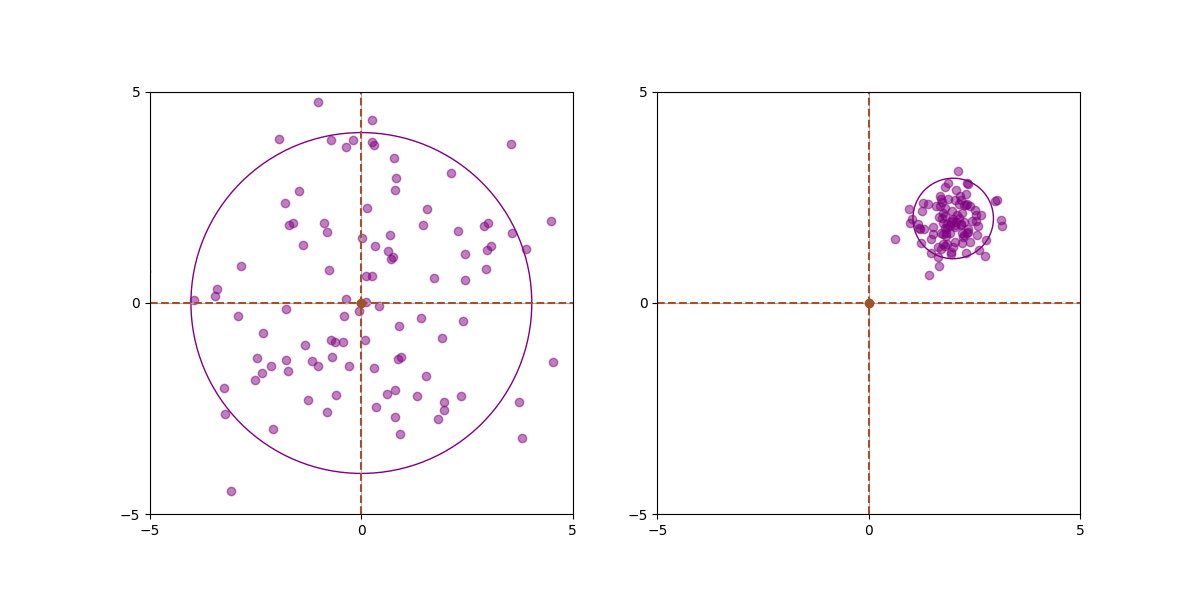
\includegraphics{images/bias-variance.webp}

\hypertarget{convergence}{%
\section{Convergence}\label{convergence}}

La dépendance du biais ou du RQ (ou d'autres indicateurs) vis à vis de
la taille de l'échantillon est une question importante :~pour une suite
d'expériences donnée, on veut que ces indicateurs tendent vite vers
zéro. Quelles sont les meilleures vitesses envisageables, et comment les
obtenir ?

Rappelons brièvement deux notions de convergence des variables
aléatoires. Une suite de variables aléatoires \(X_n\) à valeurs dans
\(\mathbb{R}^d\) converge en probabilité vers une variable aléatoire
\(X\) à valeurs dans \(\mathbb{R}^d\) si pour tout \(\varepsilon >0\),
\[
\lim_{n\to\infty} \mathbb{P} (| X_n -X|> \varepsilon ) = 0 \, .
\]

\begin{definition}[convergence d'un
estimateur]\protect\hypertarget{def-consistance}{}\label{def-consistance}

Une suite d'estimateurs \((\widehat{\theta}_n)\) est convergente pour
l'estimation de \(\theta\) lorsque, pour tout \(\theta \in \Theta\),
sous \(P_\theta\), la suite \((\hat{\theta}_n)\) converge en probabilité
vers \(\theta\) ; autrement dit, lorsque
\[ \forall \varepsilon>0, \qquad \lim_n     P_\theta ( | \widehat{\theta}_n-\theta| > \varepsilon ) =0.
\] La suite est fortement convergente si, pour tout \(\theta\), la
convergence a lieu \(P_\theta\)-presque sûrement.

\end{definition}

On voit parfois le mot \emph{consistant} utilisé au lieu de
\emph{convergent}. Je pense que c'est un anglicisme.

\hypertarget{normalituxe9-asymptotique}{%
\section{Normalité asymptotique}\label{normalituxe9-asymptotique}}

Lorsqu'un estimateur est convergent, on peut se demander à quoi
ressemblent ses fluctuations autour de sa valeur limite. Le théorème
central limite indique que le comportement asymptotique gaussiens est
relativement fréquent, et beaucoup d'estimateurs sont des sommes de
réalisations de variables indépendantes.

\begin{definition}[normalité
asymptotique]\protect\hypertarget{def-normasymp}{}\label{def-normasymp}

Soit \(\theta\) un paramètre à estimer, et \(\hat{\theta}_n\) une suite
d'estimateurs de \(\theta\). On dit que ces estimateurs sont
\emph{asymptotiquement gaussiens} (ou \emph{normaux}) si, après les
avoir renormalisés convenablement, ils convergent en loi vers une loi
gaussienne. Autrement dit, s'il existe une suite \(a_n\) de nombres
réels tels que
\[ a_n(\hat{\theta}_n - \theta) \xrightarrow[n\to \infty]{\text{loi}} N(0,\Sigma)\]
où \(\Sigma\) est une matrice de covariance qui dépend peut-être de
\(\theta\) --- pour éviter les cas dégénérés, on demande à ce que
\(\Sigma\) soit non-nulle.

\end{definition}

\hypertarget{trois-outils-sur-la-normalituxe9-asymptotique}{%
\section{Trois outils sur la normalité
asymptotique}\label{trois-outils-sur-la-normalituxe9-asymptotique}}

La normalité asymptotique n'est pas intéressante en elle-même ; l'idée
est plutôt de chercher le comportement asymptotique de la statistique
recentrée pour pouvoir en déduire des garanties en terme de risque
asymptotique ou d'intervalle de confiance. Nous le ferons souvent par la
suite : la normalité asymptotique sera par exemple utilisée pour
construire des intervalles de confiance. Aussi, prouver que des
estimateurs sont asymptotiquement normaux est une tache importante, qui
est grandement simplifiée par les deux outils suivants. On commence par
rappeler le théorème centra-limite.

\begin{theorem}[Théorème
Central-Limite]\protect\hypertarget{thm-tcl}{}\label{thm-tcl}

Soit \((X_i)\) une suite de variables aléatoires réelles, indépendantes
et identiquement distribuées. On suppose que ces variables ont une
variance \(\sigma^2\) finie. Alors, la variable aléatoire
\[ \sqrt{n}\left(\frac{1}{n}\sum_{i=1}^n X_i - \mathbb{E}[X]\right)\]
converge en loi vers une loi \(N(0,\sigma^2)\).

\end{theorem}

Le Chapitre~\ref{sec-tcl} de l'appendice revient sur différentes formes
du TCL.

Un autre lemme, dit « Lemme de Slutsky », sera fréquemment utilisé pour
combiner convergence en loi et convergence en probabilité.

\begin{theorem}[Lemme de
Slutsky]\protect\hypertarget{thm-slutsky}{}\label{thm-slutsky}

Soit \((X_n)\) une suite de variables aléatoire qui converge en loi vers
\(X\) et \((Y_n)\) une suite de variables aléatoires qui converge en
probabilité (ou en loi) vers une constante \(c\). Alors, le
\emph{couple} \((X_n, Y_n)\) converge en loi vers \((X,c)\) ; autrement
dit, pour toute fonction continue bornée \(\varphi\),
\[\mathbb{E}[\varphi(X_n, Y_n)] \to \mathbb{E}[\varphi(X,c)].\]

\end{theorem}

\begin{proof}

Fixons une fonction test \(\varphi\) continue à support compact, donc
bornée par un certain \(M\). Il faut montrer que
\(\mathbb{E}[\varphi(X_n, Y_n) - \varphi(X,c)]\) tend vers zéro.
L'intégrande est égal à la somme de
\(A = \varphi(X_n, Y_n) - \varphi(X_n, c)\) et de
\(B=\varphi(X_n, c) - \varphi(X, c)\).

Comme \(X_n\) tend en loi vers \(X\) et que \(t\to \varphi(t,c)\) est
continue bornée, l'espérance de \(B\) tend vers zéro. Il faut donc
montrer que l'espérance de \(A\) tend vers zéro. On fixe un
\(\varepsilon>0\).

\begin{itemize}
\tightlist
\item
  Par le
  \href{https://fr.wikipedia.org/wiki/Th\%C3\%A9or\%C3\%A8me_de_Heine}{théorème
  de Heine}, \(\varphi\) est uniformément continue :~il existe
  \(\delta>0\) tel que \(|(x,y) - (x', y')|<\delta\) entraîne que
  \(|\varphi(x,y) - \varphi(x', y')|< \varepsilon/2\).
\item
  On introduit l'événement \(\{|Y_n - c|\leqslant \delta\}\). Par le
  point précédent, sur cet événement on a \(|A| < \varepsilon/2\). Hors
  de cet événement, on peut toujours borner \(|A|\) par \(2M\). Le terme
  \(|\mathbb{E}A|\) est donc plus petit que
  \[\mathbb{P}(|Y_n - c|\leqslant \delta)\varepsilon/2 +  \mathbb{P}(|Y_n - c| > \delta)2M.\]
\item
  Comme \(Y_n\) converge en probabilité vers \(c\), lorsque \(n\) est
  assez grand on a \(\mathbb{P}(|Y_n - c| > \delta) < \varepsilon/4M\).
\item
  En regroupant tout ce qui a été dit, on obtient bien
  \(|\mathbb{E}A| \leqslant \varepsilon\) dès que \(n\) est assez grand,
  ce qui montre que \(\mathbb{E}A \to 0\).\\
\end{itemize}

\end{proof}

On termine par la « delta-méthode » :~si une suite d'estimateurs est
asymptotiquement normale, leur image par n'importe quelle fonction lisse
\(g\) l'est encore, et on sait calculer la moyenne et la variance
limites.

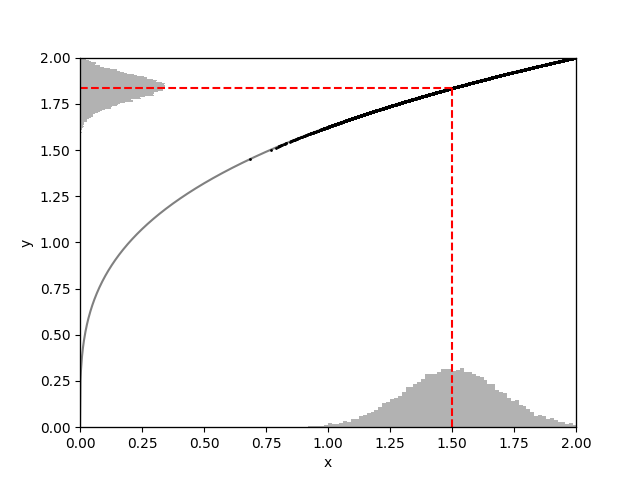
\includegraphics{images/histogram.webp}

\begin{theorem}[Delta-méthode]\protect\hypertarget{thm-deltamethod}{}\label{thm-deltamethod}

Soit \((X_n)\) une suite de variables aléatoires réelles telle que
\(\sqrt{n}(X_n - \alpha)\) converge en loi vers \(N(0,\sigma^2)\). Pour
toute fonction \(g : \mathbb{R} \to \mathbb{R}\) dérivable en \(\alpha\)
(de dérivée non nulle en \(\alpha\)), on a
\[ \sqrt{n}(g(X_n) - g(\alpha)) \xrightarrow[n \to \infty]{\text{loi}} N(0, g'(\alpha)^2 \sigma^2).\]

\end{theorem}

Plus généralement, si les \(X_n\) sont à valeurs dans \(\mathbb{R}^d\)
et que \(\sqrt{n}(X_n - \alpha) \to N(0,\Sigma)\), alors pour toute
application \(g:\mathbb{R}^d \to \mathbb{R}^k\), la suite
\(\sqrt{n}(g(X_n) - g(\alpha))\) converge en loi vers
\[N(0, Dg(\alpha)\Sigma Dg(\alpha)^\top)\] où \(Dg(x)\) est la
\href{https://fr.wikipedia.org/wiki/Matrice_jacobienne}{matrice
jacobienne} de \(g\) en \(x\).

\begin{proof}

L'approximation au premier ordre de \(g\) au point \(\alpha\) dit que
\(\sqrt{n}(g(X_n) - g(\alpha))\) est à peu près égal à
\(\sqrt{n}(X_n - \alpha)g'(\alpha)\), et comme \(g'(\alpha)\) est une
constante, ce terme converge bien en loi vers
\(N(0,\sigma^2 g'(\alpha)^2)\). Il suffit donc de montrer que le terme
de reste \(r_n\) qui complète le « à peu près » de la phrase précédente
tend lui-même vers 0. On va montrer qu'il tend bien vers 0 en
probabilité : l'application du Lemme de Slutsky ci-dessus permettra de
conclure.

La
\href{https://fr.wikipedia.org/wiki/Th\%C3\%A9or\%C3\%A8me_de_Taylor}{formule
de Taylor-Lagrange} montre qu'il y a un nombre (aléatoire) \(\xi_n\)
entre \(X_n\) et \(\alpha\) tel que le reste \(r_n\) est égal à
\[\sqrt{n}\frac{(X_n - \alpha)^2}{2}g''(\xi_n) = \frac{[\sqrt{n}(X_n - \alpha)]^2}{2\sqrt{n}}g''(\xi_n). \]

On introduit l'événement \(E_n(b) = \{|\sqrt{n}(X_n - \alpha)| < b\}\),
où \(b\) est une constante arbitraire ici. Sur cet événement,
\(|X_n - \alpha|\) est plus petit que \(b/\sqrt{n}\) donc \(X_n\) et
\(\xi_n\) tendent vers \(\alpha\), et donc \(g''(\xi_n)\) est bornée :
ainsi, sur cet événement, \(r_n\) tend vers zéro. Pour tout
\(\varepsilon >0\), on a donc
\[ \limsup_n \mathbb{P}(|r_n|>\varepsilon) \leqslant \limsup_n \mathbb{P}(\overline{E_n(b)})\]
et le terme de droite, par convergence en loi, est égale à
\(\mathbb{P}(|N(0,\sigma^2)|>b)\). Ce nombre peut être rendu
arbitrairement petit par le choix de \(b\), la limite ci-dessus est donc
nulle et on a bien \(r_n \to 0\) en probabilité.

\end{proof}

\hypertarget{deux-estimateurs-importants}{%
\section{Deux estimateurs
importants}\label{deux-estimateurs-importants}}

Deux estimateurs sont omniprésents en statistique :~la moyenne empirique
et la variance empirique. Ils sont pertinents dans n'importe quel modèle
où les observations sont des réalisations de variables iid possédant une
moyenne \(\mu\) et une variance \(\sigma^2\).

La moyenne empirique est définie par
\[ \bar{X}_n = \frac{1}{n}\sum_{i=1}^n X_i.\] Il est évident que
\(\mathbb{E}[\bar{X}_n] = \mathbb{E}[X] = \mu\). Cet estimateur est donc
toujours sans biais, et son risque quadratique est égal à sa variance,
c'est-à-dire \(\frac{\sigma^2}{n}\).

L'estimateur de la variance empirique est défini comme
\[\hat{\sigma}_n^2 = \frac{1}{n-1}\sum_{i=1}^n(X_i - \bar{X}_n)^2.\]

\begin{theorem}[]\protect\hypertarget{thm-unb}{}\label{thm-unb}

Si les \(X_i\) sont indépendants (ou simplement décorrélés),
l'estimateur \(\hat{\sigma}_n^2\) est sans biais.

\end{theorem}

\begin{proof}

Il suffit de calculer l'espérance de \((n-1)\hat{\sigma}^2_n\), ce qui
revient à calculer la somme des
\(\mathbb{E}[X_i^2 - 2X_i \bar{X}_n + \bar{X}_n^2]\). Il y a trois
éléments dans cette expression
:~\(\mathbb{E}[X_i^2], -2\mathbb{E}[X_i \bar{X}_n]\) et
\(\mathbb{E}[\bar{X}_n^2]\).

Le premier terme est égal à \(\sigma^2\). Le second terme vaut
\(-2\sum_j \mathbb{E}[X_i X_j]/n\), et tous les termes avec \(i\neq j\)
sont nuls car les \(X_k\) sont décorrélés. Il ne reste que le terme
\(j=i\), à savoir \(-2 \sigma^2 / n\). Enfin,
\(\mathbb{E}[\bar{X}_n^2]\) est la variance de \(\bar{X}_n\),
c'est-à-dire \(\sigma^2/n\).

En additionnant tout, on obtient \(\sigma^2 - \sigma^2 / n\) et comme il
y avait \(n\) termes dans la somme initiale, on obtient
\((n-1)\mathbb{E}[\hat{\sigma}_n^2] = n\sigma^2 - \sigma^2\) et donc
\(\mathbb{E}[\hat{\sigma}_n^2] = \sigma^2\).

\end{proof}

\bookmarksetup{startatroot}

\hypertarget{la-muxe9thode-des-moments}{%
\chapter{La méthode des moments}\label{la-muxe9thode-des-moments}}

Il existe plusieurs techniques générales pour \emph{construire} des
estimateurs. Deux se démarquent :~la méthode des moments, et la méthode
du maximum de vraisemblance. La méthode des moments est naturelle et
donne des estimateurs avec de bonnes propriétés, mais elle est moins
automatique que la méthode du maximum de vraisemblance que nous verrons
plus tard.

\hypertarget{quest-ce-quun-moment}{%
\section{\texorpdfstring{Qu'est-ce qu'un \emph{moment}
?}{Qu'est-ce qu'un moment ?}}\label{quest-ce-quun-moment}}

Dans un modèle statistique, supposons qu'on dispose d'une statistiques
intégrable \(T\) (pas forcément réelle), dont la moyenne n'est pas le
paramètre \(\theta\) lui-même, mais plutôt une \emph{fonction} de
\(\theta\) :\\
\[\mathbb{E}_\theta[T(X)] = \varphi(\theta).\] C'est cette fonction
\(\varphi\) qu'on appelle \emph{moment}. Typiquement,

\begin{itemize}
\tightlist
\item
  la moyenne d'une loi \(\mathscr{E}(\theta)\) n'est pas \(\theta\) mais
  \(1/\theta\).
\item
  la moyenne d'une loi log-normale de paramètres \((0, \sigma^2)\) est
  \(e^{\sigma^2/2}\).
\end{itemize}

Prenons la moyenne empirique associée à cet estimateur, \(\bar{T}_n\).
Par la loi des grands nombres,
\[\bar{T}_n = \frac{1}{n}\sum_{i=1}^n T(X_i) \to \varphi(\theta) \qquad P_\theta-ps, \]
ce qui permet d'estimer \(\varphi(\theta)\). Peut-on alors estimer
\(\theta\) ?

\hypertarget{estimateur-des-moments}{%
\section{Estimateur des moments}\label{estimateur-des-moments}}

Si la fonction \(\varphi\) est inversible et si \(\bar{T}_n\) appartient
presque sûrement à l'ensemble de définition de \(\varphi^{-1}\), alors
\(\varphi^{-1}(\bar{T_n})\) est bien définie. Pour qu'en plus cette
quantité converge presque sûrement vers \(\theta\), il faut s'assurer
que \(\varphi^{-1}\) est continue. C'est par exemple le cas lorsque
l'ensemble des paramètres \(\Theta\) est un ouvert, et que \(\varphi\)
est un difféomorphisme sur son image --- une situation si fréquente
qu'elle mérite son propre théorème, et si agréable qu'elle garantit que
l'estimateur associé est asymptotiquement normal.

\begin{theorem}[Estimation par
moments]\protect\hypertarget{thm-mom}{}\label{thm-mom}

Sous l'hypothèse mentionnée ci-dessus (la fonction \(\varphi\) est un
difféomorphisme), l'estimateur
\[\hat{\theta}_n = \varphi^{-1}(\bar{T}_n)\] est presque sûrement bien
défini pour tout \(n\) suffisamment grand ; il est également consistant
pour l'estimation de \(\theta\). En outre, si \(T\) est de carré
intégrable, cet estimateur est asymptotiquement normal, au sens où
\(\sqrt{n}(\hat{\theta}_n - \theta)\) converge en loi vers une
gaussienne centrée de matrice de variance
\[ (D\varphi(\theta))^{-1}\mathrm{Var}_\theta(T)(D\varphi(\theta)^\top)^{-1}.\]

\end{theorem}

\begin{proof}

La première partie a essentiellement été démontrée un peu plus haut.
Pour la seconde, il faut d'abord remarquer que si \(T\) est de carré
intégrable, alors \(\sqrt{n}(\bar{T}_n - \varphi(\theta))\) converge
vers une loi \(N(0, \mathrm{Var}_\theta(T))\) par le TCL. Une simple
application de la delta-méthode (Théorème~\ref{thm-deltamethod}) donne
alors le résultat, puisque la matrice jacobienne de \(\varphi^{-1}\) en
\(\varphi(\theta)\) n'est autre que l'inverse de la matrice jacobienne
de \(\varphi\) en \(\theta\).

\end{proof}

\bookmarksetup{startatroot}

\hypertarget{exercices}{%
\chapter*{Exercices}\label{exercices}}
\addcontentsline{toc}{chapter}{Exercices}

\markboth{Exercices}{Exercices}

\hypertarget{questions}{%
\section*{Questions}\label{questions}}
\addcontentsline{toc}{section}{Questions}

\markright{Questions}

\begin{enumerate}
\def\labelenumi{\arabic{enumi}.}
\tightlist
\item
  Montrer que la convergence en loi vers une constante implique la
  convergence en probabilité.
\item
  Montrer que, si un modèle statistique n'est pas identifiable, alors il
  ne peut exister aucun estimateur convergent.
\item
  Trouver un couple de variables aléatoires \((X_n, Y_n)\) tel que
  \(X_n\) converge en loi et \(Y_n\) converge en loi, mais le couple ne
  converge pas en loi.
\item
  On observe un échantillon de lois de Poisson de paramètre \(\lambda\),
  que l'on estime par la moyenne empirique. Calculer le risque
  quadratique de cet estimateur.
\item
  Quelle est la loi d'une somme de lois de Bernoulli indépendantes ?
  L'écart-type ?
\item
  Dans la delta-méthode, on demande à ce que la dérivée de \(g\) au
  point limite soit non nulle. Pourquoi ?
\item
  On se place dans le cadre de la delta-méthode, avec une suite \(X_n\)
  telle que \(\sqrt{n}(X_n - \alpha)\) converge en loi vers \(N(0,1)\).
  Si on a une fonction \(g\) telle que \(g'(\alpha)=0\) mais
  \(g''(\alpha)\neq 0\), comment renormaliser \(X_n - \alpha\) pour
  qu'on ait encore la normalité asymptotique ?
\end{enumerate}

\hypertarget{exercices-1}{%
\section*{Exercices}\label{exercices-1}}
\addcontentsline{toc}{section}{Exercices}

\markright{Exercices}

\begin{exercise}[Variance
empirique]\protect\hypertarget{exr-varemp}{}\label{exr-varemp}

On se donne \(Y_1, \dots, Y_n\), i.i.d de moyenne \(\mu\) et variance
\(\sigma^2\).

\begin{enumerate}
\def\labelenumi{\arabic{enumi}.}
\tightlist
\item
  On suppose \(\mu\) connu. Donner un estimateur non biaisé de
  \(\sigma^2\).
\item
  On suppose \(\mu\) inconnu. Calculer l'espérance de
  \(\sum_{i=1}^n (Y_i - \bar{Y}_n)^2\). En déduire un estimateur non
  biaisé de \(\sigma^2\).
\end{enumerate}

\end{exercise}

\begin{exercise}[Estimation de
masse]\protect\hypertarget{exr-tanks}{}\label{exr-tanks}

Au cours de la seconde guerre mondiale, l'armée alliée notait les
numéros de série \(X_1, \dots, X_n\) de tous les tanks nazis capturés ou
détruits, afin d'obtenir un estimateur du nombre total \(N\) de tanks
produits.

\begin{enumerate}
\def\labelenumi{\arabic{enumi}.}
\tightlist
\item
  Proposer un modèle pour le tirage de \(X_1, \dots, X_n\).
\item
  Calculer l'espérance de \(\bar X_n\). En déduire un estimateur non
  biaisé de \(N\). Indication: la loi de \(n\) tirages sans remise est
  échangeable.
\item
  Étudier la loi de \(X_{(n)}\) et en déduire un estimateur non biaisé
  de \(N\).
\item
  Proposer deux intervalles de confiance de niveau \(1-\alpha\) de la
  forme \([aS, bS]\) avec \(a, b\in\mathbb{R}\) et \(S\) une
  statistique. On pourra utiliser le fait que l'inégalité de Hoeffding
  s'applique également aux tirages sans remise.
\end{enumerate}

Selon Ruggles et Broodie (1947, JASA), la méthode statistique a fourni
comme estimation une production moyenne de 246 tanks/mois entre juin
1940 et septembre 1942. Des méthodes d'espionnage traditionnelles
donnaient une estimation de 1400 tanks/mois. Les chiffres officiels du
ministère nazi des Armements ont montré après la guerre que la
production moyenne était de 245 tanks/mois.

\end{exercise}

\begin{exercise}[Lois uniformes
(1)]\protect\hypertarget{exr-uniff1}{}\label{exr-uniff1}

On considère \((X_1, \dots, X_n)\) un échantillon de loi uniforme sur
\(]\theta, \theta+1[\).

\begin{enumerate}
\def\labelenumi{\arabic{enumi}.}
\tightlist
\item
  Donner la densité de la loi de la variable \(R_n=X_{(n)} -X_{(1)}\),
  où \(X_{(1)}=\min(X_1, \dots, X_n)\) et
  \(X_{(n)}=\max(X_1, \dots, X_n)\).
\item
  Étudier les différents modes de convergence de \(R_n\) quand
  \(n\to\infty\).
\item
  Étudier le comportement en loi de \(n(1-R_n)\) quand \(n\to\infty\).
\end{enumerate}

\end{exercise}

\begin{exercise}[Lois uniformes
(2)]\protect\hypertarget{exr-unif2}{}\label{exr-unif2}

Soit \(X_1,\dots,X_n\) un échantillon de loi
\(\mathscr{U}([0,\theta])\), avec \(\theta >0\). On veut estimer
\(\theta\).

\begin{enumerate}
\def\labelenumi{\arabic{enumi}.}
\tightlist
\item
  Déterminer un estimateur de \(\theta\) à partir de \(\bar{X}_n\).
\item
  On considère l'estimateur \(X_{(n)}= {\max}_{1\leq i \leq n}X_i\).
  Déterminer les propriétés asymotptiques de ces estimateurs.
\item
  Comparer les performances des deux estimateurs.
\end{enumerate}

\end{exercise}

\begin{exercise}[Lois
Gamma]\protect\hypertarget{exr-gamma}{}\label{exr-gamma}

La loi Gamma \(\Gamma(\alpha, \beta)\) de paramètres \(\alpha, \beta>0\)
a pour densité
\[ x\mapsto \frac{\beta^\alpha}{\Gamma(\alpha)}x^{\alpha-1}\exp(-\beta x), \quad x>0.\]
On se donne un échantillon \((X_1,\dots,X_n)\) de loi
\(\Gamma(\alpha, \beta)\) et on chercche à estimer les paramètres.

\begin{enumerate}
\def\labelenumi{\arabic{enumi}.}
\tightlist
\item
  On suppose le paramètre \(\beta\) connu. Proposer un estimateur de
  \(\alpha\) par la méthode des moments.
\item
  On suppose à présent que les deux paramètres \(\alpha, \beta\) sont
  inconnus. Proposer un estimateur de \((\alpha,\beta)\) par la méthode
  des moments.
\end{enumerate}

\end{exercise}

\begin{exercise}[Lois de
Gumbel]\protect\hypertarget{exr-gumbel}{}\label{exr-gumbel}

La loi de Gumbel (centrale) de paramètre \(\beta\) a pour fonction de
répartition \(F(x)= e^{-e^{-x/\beta}}\). On observe un échantillon de
lois de Gumbel et l'on cherche à estimer \(\beta\).

\begin{enumerate}
\def\labelenumi{\arabic{enumi}.}
\tightlist
\item
  Calculer la densité des lois de Gumbel, ainsi que leur moyenne et
  variance {[}indice :~\(0.57721…\){]}
\item
  En déduire un estimateur convergent dont on calculera le risque
  quadratique et les propriétés asymptotiques.
\end{enumerate}

\end{exercise}

\begin{exercise}[Lois de
Yule-Simon]\protect\hypertarget{exr-yule}{}\label{exr-yule}

Une variable aléatoire \(X\) suit la loi de Yule-Simon de paramètre
\(\rho>0\) lorsque \(\mathbb{P}(X = n) = \rho B(n, 1+\rho)\), où
\(n\geqslant 1\) et \(B\) est la
\href{https://en.wikipedia.org/wiki/Beta_function}{fonction beta}.

\begin{enumerate}
\def\labelenumi{\arabic{enumi}.}
\tightlist
\item
  Montrer que si \(\rho>1\), alors \(\mathbb{E}[X] = \rho/(\rho-1)\).
\item
  Trouver un estimateur de \(\rho\) et donner ses propriétés.
\end{enumerate}

\end{exercise}

\bookmarksetup{startatroot}

\hypertarget{intervalles-de-confiance}{%
\chapter{Intervalles de confiance}\label{intervalles-de-confiance}}

\hypertarget{principe}{%
\section{Principe}\label{principe}}

Dans un modèle statistique, l'estimation du paramètre d'intérêt
\(\theta\) par intervalles de confiance consiste à spécifier un
intervalle calculable à partir des données, et qui contient \(\theta\)
avec grande probabilité : en d'autres termes, une \emph{région de
confiance} pour \(\theta\).

Pour simplifier, on supposera d'abord que \(\theta\) est un paramètre
réel.

\begin{definition}[intervalle de
confiance]\protect\hypertarget{def-ic}{}\label{def-ic}

Un intervalle de confiance de niveau \(1-\alpha\) est un intervalle
\(I = [A,B]\) dont les bornes \(A,B\) sont des statistiques, et tel que
pour tout \(\theta\), \[P_\theta(\theta \in I) \geqslant 1 - \alpha.\]
Un intervalle de confiance de niveau asymptotique \(1-\alpha\) est une
\emph{suite} d'intervalles \(I_n = [A_n,B_n]\) dont les bornes
\(A_n,B_n\) sont des statistiques, et tels que pour tout \(n\),
\[ P_\theta(\theta \in I_n) \geqslant 1 - \alpha.\]

\end{definition}

Le terme « niveau » désigne \(1-\alpha\) ; la vocation de ce nombre est
d'être proche de 1, typiquement 99\%. Le nombre \(\alpha\) est parfois
appelé « erreur », « marge d'erreur » ou encore « niveau de risque » ;
la vocation de ce nombre est d'être proche de zéro, typiquement 1\%.

Il n'y a rien d'autre à savoir sur les intervalles de confiance ; tout
l'art de la chose consiste à savoir les construire. Commençons par des
exemples essentiels à plusieurs titres :~le cas d'un échantillon
gaussien, et le cas de lois de Bernoulli.

\hypertarget{exemples-gaussiens}{%
\section{Exemples gaussiens}\label{exemples-gaussiens}}

On dispose de variables aléatoires \(X_1, \dotsc, X_n\) de loi
\(N(\mu, \sigma^2)\). On va donner des intervalles de confiance pour
l'estimation des paramètres \(\mu\) et \(\sigma\) dans plusieurs cas de
figure.

\hypertarget{estimation-de-mu}{%
\subsection{\texorpdfstring{Estimation de
\(\mu\)}{Estimation de \textbackslash mu}}\label{estimation-de-mu}}

\textbf{Lorsque \(\sigma\) est connue. }

Nous avons déjà vu que la moyenne empirique \(\bar{X}_n\) est un
estimateur sans biais de \(\mu\). Or, nous savons aussi la loi
\emph{exacte} de \(\bar{X}_n\), qui est \(N(\mu, \sigma^2/n)\).
Autrement dit,
\begin{equation}\protect\hypertarget{eq-pivg}{}{\frac{\sqrt{n}}{\sigma}(\bar{X}_n - \mu) \sim N(0,1).}\label{eq-pivg}\end{equation}

Dans cette équation, on a trouvé une variable aléatoire dont la loi ne
dépend plus de \(\mu\). Il est donc possible de déterminer un intervalle
dans lequel elle fluctue à l'aide des quantiles de la loi normale, qui
sont étudiés dans Section~\ref{sec-quantiles}. Si l'on se donne une
marge d'erreur \(\alpha = 1\%\), alors
\[ \mathbb{P}( (\sqrt{n}/\sigma)|\bar{X}_n - \mu| > z_{0.99}) = 1\%\] où
\(z_{0.99} \approx 2.32\). Or,
\begin{equation}\protect\hypertarget{eq-piv1}{}{ \frac{\sqrt{n}}{\sigma}|\bar{X}_n - \mu| > z_{0.99}}\label{eq-piv1}\end{equation}
est équivalent à
\begin{equation}\protect\hypertarget{eq-piv2}{}{ \bar{X}_n - \frac{z_{0.99}\sigma}{\sqrt{n}} \leqslant \mu \leqslant \bar{X}_n + \frac{z_{0.99}\sigma}{\sqrt{n}}.}\label{eq-piv2}\end{equation}
Le passage de Équation~\ref{eq-piv1} à Équation~\ref{eq-piv2} est
souvent appelé \emph{pivot} et sert à passer d'un intervalle de
fluctuation à un intervalle de confiance.

Nous avons donc les deux bornes de notre intervalle de confiance :
\[ A = \bar{X}_n - \frac{z_{0.99}\sigma}{\sqrt{n}}\]
\[ B = \bar{X}_n + \frac{z_{0.99}\sigma}{\sqrt{n}} .\] Ces deux
quantités sont bien des statistiques, car \(\sigma\) est connu. De plus,
nous venons de montrer que \(P_\mu(\mu \in [A,B]) = 99\%\). Ici, le
choix de la marge d'erreur \(\alpha = 1\%\) ne jouait aucun rôle
particulier ; ainsi, un intervalle de confiance de niveau \(1-\alpha\)
pour l'estimation de \(\mu\) est donné par
\begin{equation}\protect\hypertarget{eq-icgmu1}{}{\left[\bar{X}_n - \frac{z_{1-\alpha}\sigma}{\sqrt{n}}~~;~~\bar{X}_n + \frac{z_{1-\alpha}\sigma}{\sqrt{n}} \right].}\label{eq-icgmu1}\end{equation}

\textbf{Lorsque \(\sigma\) est inconnue. }

Lorsque \(\sigma\) n'est pas connu, les bornes \(A,B\) ci-dessus ne sont
pas des statistiques, car elles dépendent de \(\sigma\). Heureusement,
on peut estimer \(\sigma\) sans biais via l'estimateur
\[ \hat{\sigma}_n^2 = \frac{1}{n-1}\sum_{i=1}^n (X_i - \bar{X}_n)^2.\]
Que se passe-t-il si, dans la statistique Équation~\ref{eq-pivg}, on
remplace \(\sigma\) par son estimation \(\hat{\sigma}_n^2\) ? On obtient
la statistique dite \emph{de Student},
\begin{equation}\protect\hypertarget{eq-pivst}{}{T_n = \frac{\sqrt{n}}{\sqrt{\hat{\sigma}_n^2}}(\bar{X}_n - \mu).}\label{eq-pivst}\end{equation}
Sa loi n'est plus une loi gaussienne, mais une loi de Student à \(n-1\)
paramètres de liberté \(\mathscr{T}(n-1)\):~le calcul de la densité est
fait en détails dans Section~\ref{sec-student1} -
Section~\ref{sec-student2}. Les quantiles des lois de Student ont été
calculés avec précision. On notera \(t_{k,\alpha}\) le quantile
symétrique de niveau \(\alpha\) de \(\mathscr{T}(k)\). Alors,
\[ P_{\mu, \sigma^2}(|T_n|> t_{n-1,\alpha})\leqslant \alpha .\] Par le
même raisonnement que tout à l'heure, l'inégalité
\[ \left|\frac{\sqrt{n}}{\hat{\sigma}_n}(\bar{X}_n - \mu)\right| > t_{n-1,\alpha}\]
est équivalente à
\[ \bar{X}_n - \frac{t_{n-1,\alpha}\hat{\sigma}_n}{\sqrt{n}} \leqslant \mu \leqslant \bar{X}_n + \frac{t_{n-1,\alpha}\hat{\sigma}_n}{\sqrt{n}}.\]
et les deux côtés de ces inégalités sont des statistiques;~en les notant
\(A,B\), on a bien trouvé un intervalle de confiance de niveau
\(\alpha\), c'est-à-dire tel que
\(P_{\mu,\sigma^2}(\mu \in [A,B]) = \alpha\). Cet intervalle de
confiance est d'une grande importance en pratique et mérite son propre
théorème. Il est dû à
\href{https://en.wikipedia.org/wiki/William_Sealy_Gosset}{William
Gosset}.

\begin{theorem}[Intervalle de
Student]\protect\hypertarget{thm-icg}{}\label{thm-icg}

Un intervalle de confiance de niveau \(1-\alpha\) pour l'estimation de
\(\mu\) lorsque \(\sigma\) n'est pas connue est donné par

\[\left[\bar{X}_n - \frac{t_{n-1, 1-\alpha}\hat{\sigma}_n}{\sqrt{n}}~~;~~\bar{X}_n + \frac{t_{n-1, 1-\alpha}\hat{\sigma}_n}{\sqrt{n}} \right].\]

\end{theorem}

\hypertarget{estimation-de-sigma}{%
\subsection{\texorpdfstring{Estimation de
\(\sigma\)}{Estimation de \textbackslash sigma}}\label{estimation-de-sigma}}

Supposons maintenant qu'on désire estimer la variance \(\sigma^2\).

\textbf{Lorsque \(\mu\) est connue.}

En supposant que \(\mu\) est connue, l'estimateur des moments le plus
naturel pour estimer \(\sigma^2\) est évidemment
\[ \tilde{\sigma}^2_n = \frac{1}{n}\sum_{i=1}^n (X_i - \mu)^2.\] Comme
les \((X_i - \mu)/\sigma\) sont des variables aléatoires gaussiennes
centrées réduites, l'estimateur
\(\tilde{\sigma}^2_n \times (n/ \sigma^2)\) est une somme de \(n\)
gaussiennes standard indépendantes. La loi de cette statistique est
connue :~c'est une
\href{https://fr.wikipedia.org/wiki/Loi_du_\%CF\%87\%C2\%B2}{loi du
chi-deux} à \(n\) paramètres de liberté comme démontré dans
Section~\ref{sec-chideux}. Cette loi n'est pas symétrique, puisqu'elle
est supportée sur \([0,\infty[\). On note souvent \(k^-_{n,\alpha}\) et
\(k^+_{n,\alpha}\) les nombres les plus éloignées possible (ils exisent)
tels que
\(\mathbb{P}(k^-_{n,\alpha}< \chi^2(n)<k^+_{n,\alpha}) = 1-\alpha\).
Ainsi,
\[P_{\sigma^2}(k^-_{n,\alpha}< \frac{n \tilde{\sigma}^2_n}{\sigma^2} < k^+_{n,\alpha}) = \alpha.\]
En pivotant comme dans les exemples précédents, on obtient que
l'intervalle
\[\left[\frac{n\tilde{\sigma}_n^2}{k^{+}_{n,\alpha}} ~~;~~ \frac{n\tilde{\sigma}_n^2}{k^-_{n,\alpha}} \right] \]
est un intervalle de confiance de niveau \(\alpha\) pour \(\sigma^2\).

\textbf{Lorsque \(\mu\) est inconnue.}

Cette fois, on utilise l'estimateur déjà évoqué plus tôt, à savoir
\[ \hat{\sigma}_n^2 = \frac{1}{n-1}\sum_{i=1}^n (X_i - \bar{X}_n)^2.\]
La loi de \((n-1)\hat{\sigma}^2_n / \sigma^2\) est encore une loi du
chi-deux, mais à \(n-1\) paramètres de liberté. Ainsi, le même
raisonnement que ci-dessus donne l'intervalle de confiance de niveau
\(\alpha\) suivant :~
\[\left[\frac{(n-1)\hat{\sigma}_n^2}{k^+_{n-1,\alpha}} ~~;~~ \frac{(n-1)\hat{\sigma}_n^2}{k^-_{n-1,\alpha}} \right]. \]

\hypertarget{exemples-asymptotiques}{%
\section{Exemples asymptotiques}\label{exemples-asymptotiques}}

\hypertarget{sec-icber}{%
\subsection{\texorpdfstring{Estimation du paramètre \(p\) dans un modèle
de
Bernoulli.}{Estimation du paramètre p dans un modèle de Bernoulli.}}\label{sec-icber}}

Soient \(X_1, \dotsc, X_n\) des variables indépendantes de loi
\(\mathscr{B}(p)\), dont on cherche à estimer le paramètre
\(p\in ]0,1[\). Un estimateur naturel est donné par la moyenne
empirique, \(\hat{p}_n = (X_1 + \dotsb + X_n)/n\). Cet estimateur est
non biaisé et son risque quadratique est égal à \(p(1-p)/n\). De plus,
la loi de \(\hat{p}_n\) est connue :
\(n\hat{p}_n \sim \mathrm{Bin}(n,p)\). Par conséquent, si l'on connaît
les quantiles de \(\mathscr{Bin}(n,p)-p\), on pourra construire des
intervalles de confiance de niveau \(1-\alpha\). Ces quantiles peuvent
être calculés par des méthodes numériques, mais il existe des façons
plus simples de faire.

\textbf{Inégalité BT. } L'inégalité de Bienaymé-Tchebychev dit que
\begin{equation}\protect\hypertarget{eq-btbin}{}{P_p(|\hat{p}_n - p|>t)\leqslant \frac{p(1-p)}{nt^2}. }\label{eq-btbin}\end{equation}
Si l'on choisit \[t = \sqrt{\frac{p(1-p)}{n\alpha}},\] cette probabilité
est plus petite que \(\alpha\). En pivotant, on en déduit que
l'intervalle \([\hat{p_n} \pm \sqrt{p(1-p)/n\alpha}]\) contient \(p\)
avec une probabilité supérieure à \(1-\alpha\). Mais les bornes de cet
intervalle ne sont pas des statistiques, car elles dépendent de \(p\) !
Fort heureusement, on sait que \(p\) est entre \(0\) et \(1\), ce qui
entraîne que \(p(1-p)\) est plus petit que \(1/4\), donc l'intervalle
ci-dessus est contenu dans l'intervalle plus grand
\[ \left[\hat{p}_n \pm \frac{1}{2\sqrt{n\alpha}}\right]. \] Ce dernier
est bien un intervalle de confiance de niveau \(1-\alpha\) pour
l'estimation de \(p\).

\textbf{TCL. } On a mentionné que les quantiles des lois binomiales
pourraient être calculés ; or, ils peuvent également être approchés
grâce au théorème central-limite. Celui-ci dit que
\begin{equation}\protect\hypertarget{eq-tclbin}{}{ \frac{\sqrt{n}(\hat{p}_n - p)}{\sqrt{p(1-p)}} \to N(0,1).}\label{eq-tclbin}\end{equation}
Si \(z_\alpha\) est le quantile symétrique d'ordre \(\alpha\) de
\(N(0,1)\), alors on en déduit que
\[\mathbb{P}\left(\left|\frac{\sqrt{n}(\hat{p}_n - p)}{\sqrt{p(1-p)}} \right|>z_\alpha \right) \to \alpha. \]
En pivotant, on voit alors que l'intervalle
\[\left[\hat{p}_n \pm z_\alpha \sqrt{p(1-p)/n}\right] \] contient \(p\)
avec une probabilité \emph{qui tend lorsque \(n\to\infty\) vers
\(1-\alpha\)}. Là encore, cet intervalle n'est pas un intervalle de
confiance. On pourrait utiliser deux techniques.

\begin{enumerate}
\def\labelenumi{\arabic{enumi}.}
\tightlist
\item
  Comme tout à l'heure, l'intervalle ci-dessus est contenu dans
  l'intervalle plus grand \([\hat{p}_n \pm z_\alpha/2\sqrt{n}]\) qui est
  un intervalle de confiance \emph{asymptotique} de niveau \(1-\alpha\).
\item
  Il y a plus fin. Nous savons par la loi des grands nombres que
  \(\hat{p}_n \to p\) en probabilité. Ainsi,
  \(\sqrt{\hat{p}_n(1-\hat{p}_n)} \to \sqrt{p(1-p)}\) en probabilité. Le
  lemme de Slutsky nous assure alors que dans Équation~\ref{eq-tclbin},
  on peut remplacer le dénominateur par
  \(\sqrt{\hat{p}_n (1-\hat{p}_n)}\) pour obtenir
  \begin{equation}\protect\hypertarget{eq-tclbin}{}{ \frac{\sqrt{n}(\hat{p}_n - p)}{\sqrt{\hat{p}_n(1-\hat{p}_n)}} \to N(0,1).}\label{eq-tclbin}\end{equation}
  Le reste du raisonnement est identique, et l'on obtient l'intervalle
  de confiance asymptotique de niveau \(1-\alpha\) suivant :
  \[\left[\hat{p}_n \pm z_\alpha \sqrt{\frac{\hat{p}_n(1-\hat{p}_n)}{n}}\right] \]
\end{enumerate}

\textbf{Hoeffding.} L'inégalité de Bienaymé-Tchebychev n'est pas très
fine. Il existe de nombreuses autres inégalités de concentration
:~l'inégalité de Hoeffding (Théorème~\ref{thm-hoeffding}) concerne les
variables bornées, comme ici où les \(X_i\) sont dans \([0,1]\) . Cette
inégalité dit que
\[\mathbb{P}(|\hat{p}_n - p|>t)\leqslant 2 e^{-2nt^2}. \] Le choix
\[ t = \sqrt{\frac{1}{2n}\ln\left(\frac{2}{\alpha}\right)}\] donne une
probabilité inférieure à \(\alpha\), et fournit donc l'intervalle de
confiance \textbf{non-asymptotique} de niveau \(1-\alpha\) suivant :~
\[ \left[\bar{X}_n \pm \frac{\ln(2/\alpha)}{\sqrt{2n}}\right].\]

\hypertarget{estimation-de-moyenne-dans-un-moduxe8le-non-gaussien.}{%
\subsection{Estimation de moyenne dans un modèle
non-gaussien.}\label{estimation-de-moyenne-dans-un-moduxe8le-non-gaussien.}}

Les deux techniques ci-dessus n'ont rien de spécifique au cas de
variables de Bernoulli. En fait, elles s'appliquent à tout modèle
statistique iid dont on cherche à estimer la moyenne \(\mu\), pourvu que
la variance existe.

La première méthode utilisant Bienaymé-Tchebychev nécessite de borner la
variance. Cela peut se faire dans certains cas, mais pas dans tous.

La seconde méthode s'applique systématiquement en utilisant l'estimateur
de la variance empirique \(\hat{\sigma}_n^2\). En effet, la convergence
\[\frac{\sqrt{n}}{\hat{\sigma}_n}(\bar{X}_n - \mu) \to N(0,1)\] est
toujours vraie d'après le théorème de Slutsky.

\begin{theorem}[]\protect\hypertarget{thm-icasymptcl}{}\label{thm-icasymptcl}

Soient \(X_1, \dotsc, X_n\) des variables iid possédant une variance.
L'intervalle
\[ \left[ \bar{X}_n \pm \frac{z_\alpha \hat{\sigma}_n}{\sqrt{n}} \right]\]
est un intervalle de confiance asymptotique de niveau \(\alpha\) pour
l'estimation de la moyenne des \(X_i\).

\end{theorem}

\bookmarksetup{startatroot}

\hypertarget{outils-pour-les-ic}{%
\chapter{Outils pour les IC}\label{outils-pour-les-ic}}

\hypertarget{sec-quantiles}{%
\section{Quantiles}\label{sec-quantiles}}

Si \(X\) est une variable aléatoire sur \(\mathbb{R}\), un quantile
d'ordre \(\beta \in ]0,1[\), noté \(q_\beta\), est un nombre tel que
\(\mathbb{P}(X \leqslant q_\beta) = \beta\). Lorsque \(X\) est continue,
un tel nombre existe forcément, car la fonction de répartition
\(F(x) = \mathbb{P}(X\leqslant x)\) est une surjection continue. Les
quantiles symétriques \(z_\beta\) sont, eux, définis par
\(\mathbb{P}(|X|\leqslant z_\beta) = \beta\).

Si la loi de \(X\) est de surcroît symétrique, les quantiles symétriques
s'expriment facilement en fonction des quantiles classiques. En effet,
\(\mathbb{P}(|X|\leqslant z)\) est égal à
\(\mathbb{P}(X \leqslant z) - \mathbb{P}(X \leqslant -z)\). Or, si la
loi de \(X\) est symétrique, alors
\(\mathbb{P}(X \leqslant -z) = 1 - \mathbb{P}(X \leqslant z)\), et donc
\[ \mathbb{P}(|X|\leqslant z) = 2\mathbb{P}(X \leqslant z) - 1.\] Il
suffit alors de choisir pour \(z\) le quantile \(q_{\frac{1+\beta}{2}}\)
pour obtenir \(\mathbb{P}(|X|\leqslant z) = \beta\). Lorsque \(\beta\)
est de la forme \(1-\alpha\) avec \(\alpha\) petit (comme les niveaux
des intervalles de confiance), on trouve alors
\(z_{1-\alpha} = q_{1 - \alpha/2}\).

Les quantiles s'obtiennent en inversant la fonction de répartition
:~lorsque celle-ci est une bijection sur \(]0,1[\), alors
\(q_\beta = F^{-1}(\beta)\). En règle générale, il n'y a pas de forme
fermée. Par exemple, pour une loi gaussienne standard,
\[F(x) = \frac{1}{\sqrt{2\pi}}\int_{-\infty}^x e^{-u^2/2}du\] qui
elle-même n'a pas d'écriture plus simple. Fort heureusement, les outils
de calcul numérique permettent d'effectuer ces calculs avec une grande
précision. La table suivante donne les quantiles symétriques de la
gaussienne.

\begin{longtable}[]{@{}lllllll@{}}
\toprule\noalign{}
\(\beta\) & 90\% & 95\% & 98\% & 99\% & 99.9\% & 99.99999\% \\
\midrule\noalign{}
\endhead
\bottomrule\noalign{}
\endlastfoot
\(z_\beta\) & 1.64 & 1.96 & 2.32 & 2.57 & 3.2 & 5.32 \\
\end{longtable}

Voir aussi la
\href{https://en.wikipedia.org/wiki/68\%E2\%80\%9395\%E2\%80\%9399.7_rule}{règle
1-2-3}. Il existe de nombreuses tables de quantiles pour les lois
usuelles.

\begin{theorem}[Queues de distribution de la
gaussienne]\protect\hypertarget{thm-gaussiantail}{}\label{thm-gaussiantail}

Si \(x\) est plus grand que 1,
\[  \left(\frac{1}{x} - \frac{1}{x^3}\right) \frac{e^{-x^2/2}}{\sqrt{2\pi}}\leqslant \mathbb{P}(X > x) \leqslant \frac{1}{x}\frac{e^{-x^2/2}}{\sqrt{2\pi}} \]
En particulier, si \(x\) est grand,
\(\mathbb{P}(X \geqslant x) \sim e^{-x^2/2}/x\sqrt{2\pi}\) avec une
erreur d'ordre \(O(e^{-x^2/2}/x^3)\).

\end{theorem}

À titre d'exemple, pour \(x=2.32\) cette approximation donne 98.83\%, ce
qui est remarquablement proche de 98\%. Pour \(x = 2.57\) on trouve
99.42\%.

\begin{proof}

À écrire.

\end{proof}

\hypertarget{calculs-de-lois}{%
\section{Calculs de lois}\label{calculs-de-lois}}

\hypertarget{lois-gamma-1}{%
\subsection{Lois Gamma}\label{lois-gamma-1}}

Une variable aléatoire suit une loi Gamma de paramètres
\(\lambda>0, \alpha>0\) lorsque sa densité est donnée par
\[\gamma_{r,\alpha}(x) =  \frac{\lambda^\alpha}{\Gamma(\alpha)}e^{-\lambda x}x^{\alpha -1}\mathbf{1}_{x>0}.\]
Les lois Gamma rassemblent les lois exponentielles
(\(\Gamma(\lambda, 1) = \mathscr{E}(\lambda)\)) et les lois du chi-deux
qu'on verra ci-dessous \((\Gamma(1/2, n/2) = \chi_2(n)\)). La
transformée de Fourier \(\varphi_{\lambda, \alpha}\) d'une loi
\(\Gamma(\lambda, \alpha)\) se calcule facilement par un changement de
variables :
\begin{equation}\protect\hypertarget{eq-fcgamma}{}{\varphi_{\lambda, \alpha}(t) = \left(1 - \frac{it}{\lambda}\right)^{-\alpha}.}\label{eq-fcgamma}\end{equation}
Cette identité montre également que si \(X_1, \dotsc, X_n\) sont des
variables indépendantes de loi \(\Gamma(\lambda, \alpha_i)\), alors leur
somme est une variable de loi
\(\Gamma(\lambda, \alpha_1 + \dotsc + \alpha_n)\).

\hypertarget{sec-chideux}{%
\subsection{Loi du chi-deux}\label{sec-chideux}}

Soit \(X\) une loi gaussienne standard. Calculons la densité de \(X^2\)
;~pour toute fonction-test \(\varphi\), \(\mathbb{E}[\varphi(X^2)]\) est
donné par \[\frac{1}{\sqrt{2\pi}}\int e^{-x^2/2}\varphi(x^2)dx.\] Cette
intégrale est symétrique, donc on peut ajouter un facteur 2 et intégrer
sur \([0,\infty[\). En posant \(u=x^2\), on obtient alors la valeur
\[ \frac{2}{\sqrt{2\pi}}\int_0^\infty e^{-u/2}\varphi(u)\frac{1}{2\sqrt{u}}du.\]
On reconnaît la densité d'une
\href{https://fr.wikipedia.org/wiki/Loi_Gamma}{loi Gamma} de paramètres
\((1/2, 1/2)\). Cette loi s'appelle \emph{loi du chi-deux} et on la note
\(\chi_2(1)\). Sa tranformée de Fourier est donnée par
\[\mathbb{E}[e^{itX^2}] = \frac{1}{\sqrt{1 - 2it}}. \]

Soient maintenant \(X_1,\dotsc, X_n\) des variables de loi \(N(0,1)\)
indépendantes. Chaque \(X_i^2\) est une \(\chi_2(1)\) ; leur somme a
pour loi la convolée \(n\) fois de \(\chi_2(1)\). Calculons sa
tranformée de Fourier :~
\begin{align}\mathbb{E}[e^{it(X_1^2 + \dotsb + X_n^2)}] &= \mathbb{E}[e^{itX_1^2}]^n \\ &= (1-2it)^{-\frac{n}{2}} .\end{align}
On reconnaît la transformée de Fourier d'une loi \(\Gamma(1/2, n/2)\) ;
cette loi s'appelle \emph{loi du chi-deux à \(n\) paramètres de liberté}
et elle est notée \(\chi_2(n)\). Sa densité est donnée par
\begin{equation}\protect\hypertarget{eq-chideuxdensity}{}{ \frac{1}{2^{n/2}\Gamma(n/2)}e^{-x/2}x^{n/2 - 1}\mathbf{1}_{x>0}.}\label{eq-chideuxdensity}\end{equation}

\hypertarget{sec-student1}{%
\subsection{Loi de Student}\label{sec-student1}}

Soit \(X\) une variable de loi \(N(0,1)\) et \(Y_n\) une variable de loi
\(\chi_2(n)\) indépendante de \(X\). On va calculer la loi de
\(T_n = X/\sqrt{Y_n/n}\). Soit \(\varphi\) une fonction test ;
l'espérance \(\mathbb{E}[\varphi(T_n)]\) est égale à
\[\frac{1}{Z_n\sqrt{2\pi}}\int_0^\infty \int_{-\infty}^{\infty}  \varphi\left(\frac{x}{\sqrt{y/n}}\right) e^{-\frac{x^2}{2}}e^{-\frac{y}{2}}y^{\frac{n}{2} - 1}dxdy \]
où \(Z_n = 2^{n/2}\Gamma(n/2)\). Dans l'intégrale en \(x\), on effectue
le changement de variable \(u = x/\sqrt{y/n}\) afin d'obtenir
\[\frac{1}{Z_n\sqrt{2\pi}}\int_0^\infty \int_{-\infty}^{\infty}  \varphi(u) e^{-\frac{yu^2}{2n}}e^{-\frac{y}{2}}y^{\frac{n}{2} - 1}\sqrt{\frac{y}{n}} dxdy. \]
La densité de \(T_n\) est donc donnée par
\[t_n(u)= \frac{1}{Z_n\sqrt{2\pi n}}\int_0^\infty  e^{-\frac{yu^2}{2n}-\frac{y}{2}}y^{\frac{n+1}{2}-1} dy. \]
Le changement de variables \(z = y(1+u^2/n)/2\) nous ramène à
\[t_n(u) = \frac{1}{Z_n\sqrt{2\pi n}}\left(\frac{2}{1+\frac{u^2}{n}}\right)^{\frac{n+1}{2}}\int_0^\infty  e^{-z}z^{\frac{n+1}{2}- 1} dz.\]
On reconnaît \(\Gamma((n+1)/2)\) à droite. La densité \(t_n(x)\) est
donc
\[t_n(x) = \frac{1}{\sqrt{n\pi}}\frac{\Gamma\left(\frac{n+1}{2}\right)}{\Gamma\left(\frac{n}{2}\right)}\left(\frac{1}{1 + \frac{x^2}{n}}\right)^{\frac{n+1}{2}}.\]

Cette loi s'appelle \emph{loi de Student} de paramètre \(n\) ; on dit
parfois \emph{à \(n\) degrés de liberté}. Elle est notée
\(\mathscr{T}(n)\). La loi de Student de paramètre \(n=1\) est tout
simplement une loi de Cauchy.

\hypertarget{sec-student2}{%
\subsection{Loi de la statistique de Student}\label{sec-student2}}

Soient \(X_1, \dotsc, X_n\) des variables gaussiennes
\(N(\mu, \sigma^2)\) indépendantes, et soit
\(T_n = \sqrt{n}(\bar{X}_n-\mu)/\sqrt{\hat{\sigma}^2_n}\), où
\[\hat{\sigma}^2_n = \frac{\sum_{i=1}^n (X_i - \bar{X}_n)^2}{n-1}. \]

\begin{theorem}[]\protect\hypertarget{thm-student_density}{}\label{thm-student_density}

\[T_n \sim \mathscr{T}(n-1).\]

\end{theorem}

\(~~\)

\begin{proof}

On va montrer 1° que \(\bar{X}_n\) et
\(\sqrt{\hat{\sigma}^2_n / \sigma^2}\) sont indépendantes, et 2° que
\(\sqrt{\hat{\sigma}^2_n / \sigma^2}\) a bien la même loi que
\(\sqrt{Y_{n-1}/(n-1)}\) où \(Y_{n-1}\) est une \(\chi_2(n-1)\). Dans la
suite, on supposera que \(\mu=0\) et \(\sigma=1\), ce qui n'enlève rien
en généralité.

\emph{Premier point. } Le vecteur \(X=(X_1, \dotsc, X_n)\) est gaussien.
Posons \(Z = (X_1 - \bar{X}_n, \dotsc, X_n - \bar{X}_n)\). Le couple
\((\bar{X}_n, Z_n)\) est linéaire en \(X\), donc ce couple est aussi un
vecteur gaussien. Or, la covariance de ses deux éléments est nulle. Par
exemple, \(\mathrm{Cov}(\bar{X}_n, Z_1)\) est égale à
\(\mathrm{Cov}(\bar{X}_n, X_1) - \mathrm{Var}(\bar{X}_n)\), ce qui par
linéarité donne \(1/n - 1/n = 0\). Ainsi, \(\bar{X}_n\) et \(Z\) sont
deux variables conjointement gaussiennes et décorrélées : elles sont
donc indépendantes. Comme \(\hat{\sigma}_n\) est une fonction de \(Z\),
elle est aussi indépendante de \(\bar{X}_n\).

\emph{Second point. } \(Z\) est la projection orthogonale de \(X\) sur
le sous-espace vectoriel
\(\mathscr{V}=\{x \in \mathbb{R}^n : x_1 + \dotsc + x_n = 0\}\). Soit
\((f_i)_{i=2, \dotsc, n}\) une base orthonormale de \(\mathscr{V}\), de
sorte que \(Z = \sum_{i=2}^n \langle f_i, X\rangle f_i\). Par l'identité
de Parseval, \[|Z|^2 = \sum_{i=2}^n |\langle f_i, X \rangle|^2.\] Or,
les \(n-1\) variables aléatoires \(G_i = \langle f_i, X\rangle\) sont
des gaussiennes standard iid. En effet, on vérifie facilement que
\(\mathrm{Cov}(G_i, G_j) = \langle f_i, f_j\rangle = \delta_{i,j}\). On
en déduit donc que \(|Z|^2\) suit une loi \(\chi_2(n-1)\).

\end{proof}

La seconde partie de la démonstration est un cas particulier du théorème
de Cochran, que nous verrons dans le chapitre sur la régression
linéaire.

\hypertarget{inuxe9galituxe9s-de-concentration}{%
\section{Inégalités de
concentration}\label{inuxe9galituxe9s-de-concentration}}

Les outils de base pour construire des intervalles de confiance dans des
circonstances générales (non gaussiennes) sont les inégalités de
concentration. Une inégalité de concentration pour une variable
aléatoire intégrable \(X\) consiste à borner
\(\mathbb{P}(|X - \mathbb{E}[X]|>x)\) par quelque chose de petit quand x
est grand : on cherche à contrôler la probabilité pour que les
réalisations de la variable aléatoire \(X\) soient éloignées de leur
valeur moyenne \(\mathbb{E}[X]\) de plus de \(x\).

\hypertarget{inuxe9galituxe9-de-bienaymuxe9-tchebychev}{%
\section{Inégalité de
Bienaymé-Tchebychev}\label{inuxe9galituxe9-de-bienaymuxe9-tchebychev}}

\begin{theorem}[]\protect\hypertarget{thm-bt}{}\label{thm-bt}

Soit \(X\) une variable aléatoire de carré intégrable. Alors,
\[ \mathbb{P}(|X - \mathbb{E}[X]|\geqslant x)\leqslant \frac{\mathrm{Var}(X)}{x^2}.\]

\end{theorem}

\begin{proof}

Élever au carré les deux membres de l'inégalité dans \(\mathbb{P}\),
puis appliquer l'inégalité de Markov à la variable aléatoire positive
\(|X - \mathbb{E}X|^2\) dont l'espérance est \(\mathrm{Var}(X)\).

\end{proof}

\hypertarget{inuxe9galituxe9-de-hoeffding}{%
\section{Inégalité de Hoeffding}\label{inuxe9galituxe9-de-hoeffding}}

\begin{theorem}[Inégalité de
Hoeffding]\protect\hypertarget{thm-hoeffding}{}\label{thm-hoeffding}

Soient \(X_1, \dotsc, X_n\) des variables aléatoires indépendantes, pas
forcément de même loi. On suppose que chaque \(X_i\) est à valeurs dans
un intervalle borné \([a_i, b_i]\) et on pose
\(S_n = X_1 + \dotsc + X_n\). Pour tout \(t>0\),

\begin{equation}\protect\hypertarget{eq-hoeffding}{}{\mathbb{P}(S_n - \mathbb{E}[S_n] \geqslant t) \leqslant e^{-\frac{2t^2}{\sum_{i=1}^n(b_i - a_i)^2}}}\label{eq-hoeffding}\end{equation}
et
\begin{equation}\protect\hypertarget{eq-hoeffdingsym}{}{\mathbb{P}(|S_n - \mathbb{E}[S_n]| \geqslant t) \leqslant 2e^{-\frac{2t^2}{\sum_{i=1}^n(b_i - a_i)^2}}. }\label{eq-hoeffdingsym}\end{equation}

\end{theorem}

La démonstration se fonde sur le lemme suivant.

\begin{lemma}[lemme de
Hoeffding]\protect\hypertarget{lem-hoeffding}{}\label{lem-hoeffding}

Soit \(X\) une variable aléatoire à valeurs dans \([a,b]\). Pour tout
\(t\),

\begin{equation}\protect\hypertarget{eq-lemme_hoeffding}{}{\mathbb{E}[e^{t(X-\mathbb{E}[X]}] \leqslant e^{\frac{t^2(b-a)^2}{8}}.}\label{eq-lemme_hoeffding}\end{equation}

\end{lemma}

\begin{proof}

Soit \(X\) une variable aléatoire, que par simplicité on supposera
centrée et à valeurs dans l'intervalle \([a,b]\) (\(a\) est forcément
négatif). En écrivant
\[x = a\times \frac{b-x}{b-a} + b\times \left(1 - \frac{b-x}{b-a}\right)\]
et en utilisant la convexité de la fonction \(x \mapsto e^{tx}\), on
obtient
\(e^{tX}\leqslant (b-X)e^{ta}/(b-a) + (1 - (b-x)/(b-a)) e^{bt})\), puis
en prenant l'espérance et le fait que \(X\) est centrée et en
simplifiant,
\[\mathbb{E}[e^{tX}]\leqslant \frac{be^{ta} - ae^{tb}}{b-a}.\] Notons
\(f(t)\) le terme à droite ;~pour montrer
Équation~\ref{eq-lemme_hoeffding}, il suffit de montrer que
\(\ln f(t) \leqslant t^2(b-a)^2/8\). La formule de Taylor dit que
\[ \ln f(t) = \ln f(0) + t (\ln f)'(0) + \frac{t^2}{2}(\ln f)''(\xi)\]
pour un certain \(\xi\). Or, \(\ln f(0) = \ln 1 = 0\),
\((\ln f)'(0) = f'(0)/f(0) = 0\), et il suffit donc de montrer que
\((\ln f)''(t)\) est toujours plus petit que \((b-a)^2/4\) pour
conclure. Un simple calcul montre que
\(\ln f(t) = \ln(b/(b-a)) + ta + \ln(1 - ae^{t(b-a)} / b)\), et donc
\[ (\ln f)''(t) = \frac{(a/b)(b-a)e^{t(b-a)}}{(1 - ae^{t(b-a)}/b)^2}.\]
L'inégalité \(uv/(u-v)^2 \leqslant 1/4\) appliquée à \(u = a/b\) et
\(v = e^{t(b-a)}\) permet alors de conclure.

\end{proof}

\emph{Preuve de l'inégalité de Hoeffding.} En remplaçant \(X_k\) par
\(X_k - \mathbb{E}[X_k]\), on peut supposer que tous les \(X_i\) sont
centrés et étudier seulement \(\mathbb{P}(S_n >t)\). Écrivons
\(\mathbb{P}(S_n > t) = \mathbb{P}(e^{\lambda S_n} > e^{\lambda t})\),
où \(\lambda\) est un nombre positif que l'on choisira plus tard.
L'inégalité de Markov borne cette probabilité par
\(\mathbb{E}[e^{\lambda S_n}]e^{-\lambda t}\). Comme les \(X_i\) sont
indépendantes, \(\mathbb{E}[e^{tS_n}]\) est le produit des
\(e^{ \varphi_k(\lambda)}\) où
\(\varphi_k(t) = \ln \mathbb{E}[e^{itX_k}]\). En appliquant le lemme de
Hoeffding à chaque \(\varphi_k\), on borne \(\mathbb{P}(S_n >t)\) par
\[ \exp\left(\sum_{i=1}^n \frac{(b_i - a_i)^2 \lambda^2}{8} - t\lambda\right).\]
Le minimum en \(\lambda\) du terme dans l'exponentielle est atteint au
point \(4t / \sum (a_i - b_i)^2\) et la valeur du minimum est le terme
dans l'exponentielle de Équation~\ref{eq-hoeffding}. On déduit
Équation~\ref{eq-hoeffdingsym} par une simple borne de l'union.

La démonstration de l'inégalité de Hoeffding ne dépend pas directement
du fait que \(X\) est bornée, mais plutôt de
Équation~\ref{eq-lemme_hoeffding}. Toutes les variables aléatoires qui
vérifient une inégalité de type
\(\mathbb{E}[e^{tX}]\leqslant e^{c t^2}\) pour une constante \(c\)
peuvent donc avoir leur propre inégalité de Hoeffding.

\bookmarksetup{startatroot}

\hypertarget{exercices-2}{%
\chapter*{Exercices}\label{exercices-2}}
\addcontentsline{toc}{chapter}{Exercices}

\markboth{Exercices}{Exercices}

\hypertarget{questions-1}{%
\section*{Questions}\label{questions-1}}
\addcontentsline{toc}{section}{Questions}

\markright{Questions}

\begin{enumerate}
\def\labelenumi{\arabic{enumi}.}
\tightlist
\item
  Soit \(X_n\) une variable aléatoire de loi de Student de paramètre
  \(n\). Montrer que \(X_n\) converge en loi vers \(N(0,1)\).
\item
  Soit \(X_n \sim \chi_2(n)\). La suite \((X_n)\) est-elle
  asymptotiquement normale ?
\item
  Donner un intervalle de confiance de la forme \([A,+\infty[\) pour la
  moyenne d'un échantillon gaussien.
\item
  Même question pour la variance dans un modèle gaussien centré.
\item
  Dans l'estimation de la moyenne \(\mu\) d'un modèle gaussien où la
  variance \(\sigma^2\) est connue, montrer que l'intervalle de
  confiance obtenu (Équation~\ref{eq-icgmu1}) est le plus grand possible
  de niveau \(1-\alpha\).
\item
  Démontrer le théorème Théorème~\ref{thm-gaussiantail} sur
  l'asymptotique des queues de distribution de la loi gaussienne.
\item
  Montrer la borne suivante sur les quantiles de loi gaussienne
  standard:~\(q_\beta < \sqrt{\ln\frac{1}{\beta\sqrt{2\pi}}}\) (pour
  tout \(1/2<\beta<1\)).\\
\item
  Comparer les queues de distribution des lois \(N(0,1), \chi_2(n)\) et
  \(\mathscr{T}(n)\).
\item
  Expliquer à votre grand-mère la différence entre un intervalle de
  fluctuation et un intervalle de confiance.
\item
  L'intervalle de confiance de niveau \(1-\alpha\) pour la moyenne d'un
  modèle \(N(\mu, 1)\) avec \(n\) observations est
  \(I_n = [\bar{X}_n \pm z_\alpha /\sqrt{n}]\). Supposons qu'on obtienne
  une nouvelle observation indépendante des autres, disons \(Z\). La
  probabilité \(\mathbb{P}(Z \in I_n)\) est-elle plus grande ou plus
  petite que \(1-\alpha\) ?
\item
  Comparer la longueur des intervalles de confiance obtenus par les
  différentes méthodes de la section Section~\ref{sec-icber}.
\item
  Le quantile d'ordre 97,5\% d'une variable
  \(X\sim \mathrm{Bin}(12,1/2)\) est 9. Trouver \(c\) tel que
  \(\mathbb{P}(|X-6|>c)=95\%\).
\end{enumerate}

\hypertarget{exercices-3}{%
\section*{Exercices}\label{exercices-3}}
\addcontentsline{toc}{section}{Exercices}

\markright{Exercices}

\begin{exercise}[Lois de
Poisson]\protect\hypertarget{exr-poisson}{}\label{exr-poisson}

On suppose que l'on observe \(X_1, \dots, X_n\) i.i.d de loi
\(\mathscr{P}(\theta)\).

\begin{enumerate}
\def\labelenumi{\arabic{enumi}.}
\tightlist
\item
  Étudier \(\bar{X}_n\).
\item
  Montrer que
  \(\sqrt{\bar{X}_n} \underset{n \rightarrow \infty}{\overset{\mathbb{P}}{\longrightarrow}} \sqrt{\theta}\).
\item
  Donner deux intervalles de confiance au niveau \(98 \%\) pour
  \(\sqrt{\theta}\), et les comparer.
\end{enumerate}

\end{exercise}

\begin{exercise}[Lois
uniformes]\protect\hypertarget{exr-unif}{}\label{exr-unif}

Soit \(X_1, \dotsc, X_n\) des variables aléatoires iid de loi
\(\mathscr{U}[0,\theta]\). Donner un intervalle de confiance non
asymptotique pour \(\theta\) en utilisant l'estimateur
\(\hat{\theta}_n = \max_{i=1,\dotsc, n}X_i\).

\end{exercise}

\begin{exercise}[Lois exponentielles
décalées]\protect\hypertarget{exr-expodec}{}\label{exr-expodec}

Soit \(X_1, \dotsc, X_n\) des variables aléatoires iid de densité
\(e^{\theta-x} \mathbf{1}_{x>\theta}\), où \(\theta >0\).

\begin{enumerate}
\def\labelenumi{\arabic{enumi}.}
\tightlist
\item
  Calculer \(\mathbb{E}_\theta\left[X_1\right]\) et en déduire un
  estimateur de \(\theta\) que l'on notera \(\hat\theta_n\). Étudier ses
  propriétés (risque quadratique, convergence) et l'utiliser pour
  construire un premier intervalle de confiance \(I_1(\alpha)\)
  non-asymptotique pour \(\theta\) de niveau \(1-\alpha\).
\item
  Construire un intervalle de confiance asymptotique \(I_2(\alpha)\)
  pour \(\theta\) à partir de \(\hat{\theta}_n\).
\item
  Montrer que l'estimateur
  \(\theta_n^\star := \min_{1 \leq i \leq n} X_i\) est meilleur que
  \(\hat \theta_n\) au sens du risque quadratique, puis l'utiliser pour
  construire un intervalle de confiance \(I_3(\alpha)\) de niveau
  \(1-\alpha\).
\item
  Comparer les longueurs de tous ces différents intervalles de
  confiance.
\end{enumerate}

\end{exercise}

\begin{exercise}[Lois
exponentielles]\protect\hypertarget{exr-expo}{}\label{exr-expo}

Soit \(X_1, \dotsc, X_n\) des variables aléatoires iid exponentielles de
paramètre \(\lambda>0\).

\begin{enumerate}
\def\labelenumi{\arabic{enumi}.}
\tightlist
\item
  Quelle est la loi de \(S_n = X_1 + \dotsb + X_n\) ?
\item
  Construire un intervalle de confiance de niveau \(1-\alpha\) pour
  \(\lambda\).
\end{enumerate}

\end{exercise}

\begin{exercise}[Inégalité
d'Azuma]\protect\hypertarget{exr-azuma}{}\label{exr-azuma}

Montrer que l'inégalité de Hoeffding reste valable lorsque les \(X_i\)
ne sont plus supposés indépendants, mais que la suite
\(S_k = X_1 + \dotsb + X_k\) est une martingale. Indice :
\(\mathbb{E}[e^{\lambda S_{n+1}}] = \mathbb{E}[e^{\lambda S_n}\mathbb{E}[e^{\lambda X_{n+1}}|S_n]]\).

Ce raffinement s'appelle \emph{inégalite de Hoeffding-Azuma}. C'est
celui que nous avons utilisé dans l'exercice (\textbf{ex-tanks?}),
lorsque les \(X_1, \dotsc, X_n\) sont des tirages \emph{sans remise}
dans une urne à \(N\) éléments.

\end{exercise}

\bookmarksetup{startatroot}

\hypertarget{test-dhypothuxe8ses}{%
\chapter{Test d'hypothèses}\label{test-dhypothuxe8ses}}

Si l'on essaie d'estimer le rendement \(\mu\) d'un actif financier, on
cherche implicitement à savoir si l'on va investir ou pas. Cette
décision dépendra de notre estimation : pour faire simple, on peut
considérer que si nous estimons que le rendement est positif
(\(\hat{\mu}>0\)), alors il faut investir. Sinon, on n'investira pas.

Les tests d'hypothèses visent à formaliser cela. Faire une
\emph{hypothèse} dans un modèle statistique
\((\mathcal{X}, \mathscr{F}, (P_\theta)_{\theta \in \Theta_0})\), c'est
supposer que \(\theta\) appartient à une certaine région de
\(H_0 \subset \Theta\). Les \emph{tests} visent à construire des
procédures pour tester une hypothèse nulle, que l'on notera \(H_0\),
contre une hypothèse alternative, notée \(H_1\).

Dans le cadre ci-dessus, on peut se placer dans un modèle où les
rendements sont \(\mathscr{N}(\mu, \sigma^2)\). On veut tester
l'hypothèse nulle \(H_0 : \mu \in ]-\infty, 0]\) contre l'hypothèse
alternative \(H_1 : \mu \in ]0,+\infty[\).

\newcommand{\rejet}{\mathsf{rejeter}}
\newcommand{\accept}{\mathsf{accepter}}

\begin{definition}[]\protect\hypertarget{def-test}{}\label{def-test}

Un test est un événement qui, s'il survient, nous incite à rejeter
l'hypothèse nulle. Cet événement sera noté \(\mathsf{rejeter}\) et son
complémentaire sera noté \(\mathsf{accepter}\).

\begin{itemize}
\item
  L'erreur de première espèce est la probabilité de rejeter l'hypothèse
  nulle à tort :
  \(\alpha = \sup_{\theta \in H_0}P_\theta(\mathsf{rejeter})\). Le
  \textbf{niveau d'un test} est \(1-\alpha\). C'est la probabilité
  d'accepter l'hypothèse nulle à raison.
\item
  L'erreur de seconde espèce est la probabilité de ne pas rejeter
  l'hypothèse nulle, à tort :
  \(\beta = \sup_{\theta \in H_1}P_\theta(\mathsf{accepter})\). La
  \textbf{puissance d'un test} est \(1-\beta\). C'est la probabilité de
  « détecter » l'hypothèse alternative à raison.
\item
  L'affinité d'un test est la somme des erreurs de première et seconde
  espèce. On parle aussi de l'\emph{erreur totale}.
\end{itemize}

\end{definition}

Par « événement », on veut bien dire « un élément de \(\mathscr{F}\) »,
c'est-à-dire qui n'est déterminé que par les observations et pas par
\(\theta\). Formellement on écrit souvent qu'un test est une
statistique, disons \(T\), à valeurs dans \(\{0,1\}\). L'événement
\(\{T=1\}\) est \(\mathsf{rejeter}\), l'événement \(\{T=0\}\) est
\(\mathsf{accepter}\).

Un des grands objectifs de la statistique mathématique est de construire
des familles de tests qui, pour un niveau de confiance \(1-\alpha\)
fixé, ont la plus grande puissance possible ; autrement dit,
\textbf{trouver un événement hautement improbable sous l'hypothèse
nulle, et hautement probable sous l'hypothèse alternative}.

Comme on verra dans les exemples, le rôle des deux hypothèses n'est pas
interchangeable. Maximiser le niveau et la puissance ne reviennent pas
au même. Le choix des hypothèses \(H_0\) et \(H_1\) n'est pas anodin
:~l'hypothèse \(H_0\) est une hypothèse que l'on cherche implicitement à
réfuter.

\begin{enumerate}
\def\labelenumi{\arabic{enumi}.}
\tightlist
\item
  Si \(\theta \in H_0\) quel qu'il soit, les probablités pour qu'un
  certain événement \(\mathsf{rejeter}\) sont infimes -- disons, 1\%.
\item
  Si cet événement arrive, par contraposée, on est amenés à rejeter
  l'hypothèse selon laquelle \(\theta\) est dans \(H_0\).
\end{enumerate}

C'est pour cela que les tests sont une forme de logique statistique. Le
raisonnement de base une contraposée :~en logique, \(A \Rightarrow B\)
est équivalent à \(\neg B \Rightarrow \neg A\). En statistiques, on
pourrait écrire \(\theta \in H_0 \Rightarrow \mathsf{accepter}\) (avec
grande probabilité), donc
\(\mathsf{rejeter}\Rightarrow \theta \notin H_0\) (probablement).

\hypertarget{exemples-de-tests-gaussiens}{%
\section{Exemples de tests
gaussiens}\label{exemples-de-tests-gaussiens}}

On se place dans un modèle où \(X_1, \dotsc, X_n\) sont des gaussiennes
\(N(\mu, \sigma^2)\). Nous avons déjà vu plusieurs fois que
\(\bar{X}_n \sim N(\mu, \sigma^2/n)\).

\hypertarget{construction-du-test}{%
\subsection{Construction du test}\label{construction-du-test}}

On cherche à réfuter l'hypothèse selon laquelle ces variables aléatoires
sont centrées ; autrement dit, on posera \(H_0 = \{\mu=0\}\). Sous cette
hypothèse, nos variables aléatoires sont donc des variables
\(N(0,\sigma^2)\).

\textbf{Supposons dans un premier temps que \(\sigma^2\) est connue.}
Sous \(H_0\), on a donc
\[ \frac{\sqrt{n}\bar{X}_n}{\sigma} \sim N(0,1)\] et par conséquent,
\(P_0(|\bar{X}_n| < z_{1-\alpha} \sigma / \sqrt{n}) = 1-\alpha\).
Autrement dit, sous l'hypothèse \(\mu = 0\), on devrait observer
l'événement
\[ \bar{X}_n \in \left[ \pm \frac{z_{1-\alpha} \sigma}{\sqrt{n}}\right]\]
avec probabilité élevée \(1-\alpha\). Si cet événement n'est pas
observé, il est alors très douteux que \(\mu\) soit effectivement égal à
zéro !~On pose donc
\[ \mathsf{rejeter}_\alpha = \{|\bar{X}_n | > z_{1-\alpha} \sigma / \sqrt{n}\}.\]
Le niveau de ce test est bien \(1-\alpha\) : nous l'avons construit pour
cela.

\textbf{Supposons maintenant que \(\sigma\) n'est pas connue.} En
l'estimant via \(\hat{\sigma}_n\), nous savons que (toujours sous
l'hypothèse selon laquelle \(\mu=0\))
\[ \frac{\sqrt{n}\bar{X}_n}{\hat{\sigma}_n} \sim \mathscr{T}(n-1).\] On
reproduit alors le raisonnement ci-dessus : comme
\(\mathbb{P}(|\bar{X}_n| < t_{n-1, 1-\alpha}\hat{\sigma}_n / \sqrt{n}) = \alpha\)
où \(t_{n-1,1-\alpha}\) est le quantile symétrique de
\(\mathscr{T}(n-1)\), on voit que l'événement
\[ \mathsf{rejeter}_\alpha = \{|\bar{X}_n| > t_{n-1,1-\alpha}\hat{\sigma}_n / \sqrt{n}\}\]
est bien un test de niveau \(1-\alpha\).

\hypertarget{calcul-de-la-puissance-et-hypothuxe8se-alternative}{%
\subsection{Calcul de la puissance et hypothèse
alternative}\label{calcul-de-la-puissance-et-hypothuxe8se-alternative}}

Nous n'avons pas encore eu besoin de spécifier une hypothèse
alternative, mais nous allons en avoir besoin pour calculer la puissance
du test. Pour commencer, on va supposer que, si \(\mu\) n'est pas nulle,
alors elle ne peut être égale qu'à 1. Autrement dit, \(H_1 = \{1\}\). Ce
genre d'hypothèse alternative ne peut évidemment avoir de pertinence
qu'en fonction du problème réel sous-jacent !

Sous l'hypothèse alternative, donc, nous savons que
\(\bar{X}_n \sim N(1, \sigma^2)\). La puissance du test est définie par
\(1-\beta\) où \(\beta=P_1(\mathsf{accepter}_\alpha)\) c'est-à-dire
\begin{align}\beta &= P_1(|\bar{X}_n|\leqslant z_{1-\alpha} \sigma / \sqrt{n}) \\
&= P_1 \left(-\frac{z_{1-\alpha} \sigma}{\sqrt{n}}\leqslant \bar{X}_n \leqslant \frac{z_{1-\alpha} \sigma}{\sqrt{n}} \right) \\
&= P_1 \left(-\frac{z_{1-\alpha} \sigma}{\sqrt{n}}-1\leqslant \bar{X}_n - 1 \leqslant \frac{z_{1-\alpha} \sigma}{\sqrt{n}} -1 \right)\\
&= \Phi(-\sqrt{n}/\sigma + z_{1-\alpha}) - \Phi(-\sqrt{n}/\sigma + z_{1-\alpha}).
\end{align} où \(\Phi(x) = \mathbb{P}(N(0,1)\leqslant x)\). Cette
expression ne peut pas plus se simplifier, mais on peut quand même la
borner par \(F(-\sqrt{n}/\sigma + z_{1-\alpha})\). Lorsque \(x\) est
grand, nous avons vu (Théorème~\ref{thm-gaussiantail}) que
\(F(x) < e^{-x^2}/|x|\sqrt{2\pi}\). Ainsi, l'erreur de première espèce
est bornée par \(O(e^{-n/\sigma^2/2} / \sqrt{n})\). Cela tend
extrêmement vite vers 0 ;~en fait, dès que \(n\) est plus grand que 10
et \(\sigma=1\), cette erreur est inférieure à 0.1\%, donc dans ce cas
le test aura une puissance supérieure à \(99.9\%\).

Que se serait-il passé si notre hypothèse alternative n'avait pas été
\(\mu=1\) mais \(\mu = m\) pour n'importe quel \(m\neq 0\) ? Dans ce
cas, on aurait eu \(H_1 = \mathbb{R}\setminus \{0\}\). L'erreur de
première espèce aurait alors été \(\beta = \sup_{m\neq 0}\beta_m\) où
\[ \beta_m = P_m(\mathsf{accepter}_\alpha).\] On revoyant les calculs
ci-dessus, on voit que
\[\beta_m = \Phi(-m\sqrt{n}/\sigma + z_{1-\alpha}) - \Phi(-m\sqrt{n}/\sigma + z_{1-\alpha}).\]
En particulier,
\[\lim_{m\to 0}\beta_m =\Phi(-z_{1-\alpha}) - \Phi(-z_{1-\alpha}) =  1-\alpha\]
par continuité de \(\Phi\) et par définition de \(z_{1-\alpha}\). Ainsi,
\(1-\beta = \alpha\) :~pour cette seconde hypothèse alternative, la
puissance de notre test\ldots{} est extrêmement faible.

\textbf{Cela vient du fait que notre hypothèse alternative contient des
situations quasiment indiscernables de notre hypothèse nulle.} Par
exemple, il est quasiment impossible de distinguer \(\mu = 0\) de
\(\mu = 10^{-100}\) par exemple. Cet exemple illustre la dissymétrie
entre \(H_0\) et \(H_1\).

\hypertarget{la-notion-de-p-valeur}{%
\section{\texorpdfstring{La notion de
\(p\)-valeur}{La notion de p-valeur}}\label{la-notion-de-p-valeur}}

La construction d'un test dépend du niveau de risque \(\alpha\). Si le
niveau de risque acceptable est de plus en petit, alors l'événement
\(\mathsf{rejeter}_\alpha\) devrait être de moins en moins probable.
D'ailleurs, \(\mathsf{rejeter}_0 = \varnothing\) et
\(\mathsf{accepter}_0 = \Omega\) : si l'on ne tolère aucun niveau de
risque de première espèce, c'est qu'on ne veut pas rejeter l'hypothèse
nulle.

Très souvent, si \(\alpha<\beta\), on a même
\[\mathsf{rejeter}_\alpha \subset \mathsf{rejeter}_\beta.  \]

\begin{definition}[]\protect\hypertarget{def-pval}{}\label{def-pval}

La \(p\)-valeur d'une famille croissante de tests est le plus petit
niveau de risque qui nous amène à rejeter l'hypothèse nulle compte tenu
des observations. Formellement,
\[ p_\star = \inf\{\alpha>0 : \mathsf{rejeter}_\alpha\} = \sup\{\alpha>0 : \mathsf{accepter}_\alpha\}.\]

\end{definition}

\textbf{La \(p\)-valeur dépend des observations.} C'est une observation
cruciale : la \(p\)-valeur n'est pas une propriété intrinsèque d'un
test. Sur deux ensembles différents d'observations, la \(p\)-valeur ne
sera pas la même en général.

\textbf{Calcul de \(p\)-valeur.} Dans de nombreux tests, la construction
d'un test se fonde sur une statistique, disons \(S\), qui sous
l'hypothèse nulle suit une loi particulière (par exemple,
\(\sqrt{n}\bar{X}_n / \hat{\sigma}_n \sim \mathscr{T}(n-1)\) sous
l'hypothèse \(X_i \sim N(\mu,\sigma^2)\) avec \(\mu=0\) dans le cas d'un
test de Student). Si le test est de la forme \(S < q_{1-\alpha}\), ce
qui équivaut à \(F(S)<1-\alpha\). La \(p\)-valeur est donnée par
\[p_\star = \sup\{\alpha > 0 : S < q_{1-\alpha}\} = \sup\{\alpha : F(S)<1-\alpha\} = 1 - F(S).\]

\bookmarksetup{startatroot}

\hypertarget{thuxe9orie-des-tests-simples}{%
\chapter{Théorie des tests simples}\label{thuxe9orie-des-tests-simples}}

\hypertarget{la-distance-en-variation-totale}{%
\section{La distance en variation
totale}\label{la-distance-en-variation-totale}}

Lorsqu'on cherche à tester une hypothèse de type \(\text{loi} = P\)
contre une hypothèse de type \(\mathrm{loi} = Q\) (c'est-à-dire, deux
hypothèses simples), on en revient à chercher un événément très
improbable sous la loi \(P\), et très probable sous la loi \(Q\). On
peut se demander en toute généralité quels sont les événements pour
lesquels ces probabilités diffèrent le plus, c'est-à-dire les événements
\(A\) qui maximisent \(P(A) - Q(A)\). Cela mène directement à la
définition de la \emph{variation totale}.

\begin{definition}[distance en variation
totale]\protect\hypertarget{def-dtv}{}\label{def-dtv}

Soient \(P,Q\) deux mesures de probabilité sur un même espace
\((\mathcal{X}, \mathscr{F})\). Leur distance en variation totale est
\[ \dtv(P,Q) = \sup_{A \in \mathscr{F}}P(A) - Q(A). \]

\end{definition}

La distance en variation totale est un objet important en probabilités,
qui possède de nombreuses propriétés. Parmi elles, voici les plus
importantes.

\begin{enumerate}
\def\labelenumi{\arabic{enumi}.}
\tightlist
\item
  C'est une distance sur l'espace des mesures de probabilité.
\item
  Elle génère une topologie plus fine que celle de la convergence en loi
  ;~autrement dit, si \(\dtv(P_n, Q) \to 0\) alors \(P_n\) converge en
  loi vers \(Q\) mais l'inverse n'est pas vrai.
\end{enumerate}

\begin{proposition}[]\protect\hypertarget{prp-dtv}{}\label{prp-dtv}

Soit \(\nu\) une mesure telle que \(P\) et \(Q\) sont absolument
continues\footnote{Si \(P\) est
  \href{https://fr.wikipedia.org/wiki/Th\%C3\%A9or\%C3\%A8me_de_Radon-Nikodym-Lebesgue}{absolument
  continue} par rapport à \(Q\) (ce qu'on note \(P \ll Q\)), alors la
  dérivée de Radon-Nikodym existe, et c'est une fonction mesurable
  positive \(f\) (unique à un ensemble \(Q\)-négligeable près) qui
  vérifie \(P(A) = \int f(x)\mathbf{1}_{x\in A}\mathrm{d}Q\). On appelle
  cette fonction \emph{densité} de \(P\) par rapport à \(Q\).} par
rapport à \(\nu\), de densités respectives \(p\) et \(q\) par rapport à
\(\nu\). Alors, \(\dtv(P,Q)\) est égale à chacune des quantités
suivantes :

\[\int_{\mathcal{X}} (p(x) - q(x))_+\mathrm{d}\nu\]
\begin{equation}\protect\hypertarget{eq-dtvformule}{}{ \frac{1}{2}\int_{\mathcal{X}} |p(x) - q(x)|\mathrm{d}\nu.}\label{eq-dtvformule}\end{equation}

De plus, notons \(E\) l'ensemble mesurable
\(\{x \in \mathcal{X} : p(x)>q(x)\}\). Alors,
\begin{equation}\protect\hypertarget{eq-dtv-2}{}{\dtv(P,Q) = P(E) - Q(E).}\label{eq-dtv-2}\end{equation}

\end{proposition}

L'hypothèse selon laquelle \(P,Q\) sont a.c. par rapport à \(\nu\) est
toujours vérifiée pour \(\nu = (P+Q)/2\), et n'est donc pas restrictive.

\begin{proof}

Pour tout événement \(A \in \mathscr{F}\), la différence \(P(A) - Q(A)\)
est égale à \(\int_A p(x) - q(x) \mathrm{d}\nu\), qui peut elle-même
s'écrire sous la forme
\[\int_{A \cap E} (p - q) \mathrm{d}\nu + \int_{A \cap \bar{E}} (p - q) \mathrm{d}\nu.\]
Le second terme est négatif, puisque si \(x \notin E\) alors
\(p(x)\leqslant q(x)\). Ainsi, \(P(A) - Q(A)\) est plus petit que le
premier terme, lequel est à son tour plus petit que
\(\int_E (p-q)d\nu = P(E) - Q(E)\). Cela montre directement
Équation~\ref{eq-dtv-2}. Au passage, il est évident que
\[\int_E (p(x)-q(x))\mathrm{d}\nu = \int_{\mathcal{X}}(p(x) - q(x))_+ \mathrm{d}\nu,  \]
ce qui montre la première égalité de Équation~\ref{eq-dtvformule}. La
seconde égalité résulte de la première, puisque comme \(p\) et \(q\)
sont des densités de probabilité, on a forcément
\(\int (p-q)_+ = \int(p-q)_-\).

\end{proof}

Dans la suite, on supposera toujours que les diverses lois possèdent
toutes une densité par rapport à une mesure de référence \(\nu\). C'est
le cas dans de très nombreux modèles --- pas tous, hélas. Les lettres
majuscules désigneront les mesures, tandis que les lettres minuscules
désigneront leurs densités.

\hypertarget{test-optimal-au-sens-de-laffinituxe9}{%
\section{Test optimal au sens de
l'affinité}\label{test-optimal-au-sens-de-laffinituxe9}}

L'affinité d'un test est la somme de ses erreurs de première et seconde
espèce :~c'est la probabilité de « se tromper » en général, quelle que
soit l'hypothèse.

\newcommand{\reject}{\mathsf{rejeter}}

\begin{theorem}[]\protect\hypertarget{thm-affinity}{}\label{thm-affinity}

Soit \(\mathfrak{T}\) l'ensemble des tests possibles de l'hypothèse
\(H_0 : P = P_0\) contre l'hypothèse alternative \(H_1 : P = P_1\).
Alors, le test possédant la meilleure affinité possible parmi tous les
tests possibles vérifie
\[\inf_{T \in \mathfrak{T}}~\{\alpha_T + \beta_T \} = 1 - \dtv(P_0, P_1). \]
En particulier, le test optimal pour l'affinité est donné par la région
de rejet \[ \mathsf{rejeter}_\star = \{p_0(x) < p_1(x)\}.\]

\end{theorem}

\begin{proof}

Soit \(T\) n'importe quel test. Son affinité est
\(P_1(\{T=0\}) + P_0(\{T=1\})\). En passant au complémentaire dans le
second terme, on obtient \[1 - (P_0(\{T=0\}) - P_1(\{T=0\})). \] Cette
quantité est forcément plus petite que \(1 - \dtv(P_0, P_1)\) par la
définition même de la variation totale. De plus, cette borne est
atteinte en choisissant le test \(T\) donné dans l'énoncé, d'où
l'égalité.

\end{proof}

\textbf{Commentaire.} Le théorème précédent semble donner au problème de
la construction de tests une réponse définitive :~il donne le test
optimal au sens de l'affinité, test qui est élémentaire et intuitif. En
effet, si \(P_0, P_1\) sont les deux lois et si \((x_1, \dotsc, x_n)\)
est l'échantillon observé, alors on rejette l'hypothèse nulle si la
probabilité de cette observation est plus grande sous \(P_1\) que sous
\(P_0\) : autrement dit, si
\[ \frac{p_1(x_1, \dotsc, x_n)}{p_0(x_1, \dotsc, x_n)}>1. \] Le terme de
droite s'appelle \textbf{rapport de vraisemblance}. Pourtant, ce test ne
permet pas de contrôler l'erreur de première espèce. Il peut tout à fait
exister d'autres tests qui ont un niveau plus élevé. Il est donc naturel
de se demander si, parmi les tests ayant un niveau fixé \(1-\alpha\), il
existe un autre critère d'optimalité.

\hypertarget{thuxe9oruxe8me-de-neyman-pearson}{%
\section{Théorème de
Neyman-Pearson}\label{thuxe9oruxe8me-de-neyman-pearson}}

On se place toujours dans un cadre où les deux lois \(P_0\) et \(P_1\)
possèdent deux densités \(p_0, p_1\) par rapport à une mesure commune
\(\nu\).

\begin{definition}[]\protect\hypertarget{def-testRV}{}\label{def-testRV}

Un \emph{test du rapport de vraisemblance} est un test dont la région de
rejet est de la forme
\begin{equation}\protect\hypertarget{eq-rejetMV}{}{\mathsf{rejeter}= \left\lbrace \frac{p_1(x)}{p_0(x)} > z \right\rbrace }\label{eq-rejetMV}\end{equation}
pour un certain \(z>0\).

\end{definition}

Le test optimal au sens de l'affinité est un test de rapport de
vraisemblance (\(z=1\)).

\begin{theorem}[Théorème de
Neyman-Pearson]\protect\hypertarget{thm-jerzy}{}\label{thm-jerzy}

Tout test de même niveau qu'un test du rapport de vraisemblance est
moins puissant que celui-ci.

\end{theorem}

\begin{proof}

On suppose que la région de rejet de \(T_\star\) est de la forme
Équation~\ref{eq-rejetMV}. Soit \(T\) un autre test de même niveau que
\(T_\star\). La quantité
\[ \int_{\mathcal{X}} (T(x) - T_\star(x))(p_1(x) - z p_0(x))\mathrm{d}\nu \]
est forcément négative ou nulle : en effet, si \(T_\star(x)=1\), alors
\(T(x)-T_\star(x) = T(x)-1 \leqslant 0\), mais \(p_1(x)\) est plus grand
que \(zp_0(x)\), donc \((p_1(x) - zp_0(x))\geqslant 0\). De même, si
\(T(x) = 0\), alors cette fois ce terme est négatif. Dans les deux cas,
la fonction dans l'intégrale est toujours le produit de deux nombres de
signes opposés : elle est donc négative. Or, en développant cette
intégrale, on constate qu'elle vaut aussi
\[P_1(T=1) - P_1(T_\star=1) - zP_0(T=1)+zP_0(T_\star=1). \] Tout ceci
n'est rien d'autre que \(\beta_\star-\beta - z(\alpha-\alpha_\star)\),
où \(\alpha, \beta\) désignent les deux types d'erreurs du test \(T\) et
\(\alpha_\star, \beta_\star\) celles de \(T_\star\). Mais nous avons
supposé que \(\alpha = \alpha_\star\) : des deux termes ci-dessus, ne
reste que le premier, à savoir \(\beta_\star - \beta\), qui est bien
négatif comme demandé.

\end{proof}

\hypertarget{un-exemple-de-test-de-rapport-de-vraisemblance}{%
\section{Un exemple de test de rapport de
vraisemblance}\label{un-exemple-de-test-de-rapport-de-vraisemblance}}

Plaçons-nous dans un modèle de Bernoulli :~on a des variables aléatoires
\(X_1, \dotsc, X_n\) iid de loi \(\mathrm{Ber}(p)\), et l'on souhaite
tester une valeur \(p_0\) de \(p\) contre une valeur \(p_1 \neq p_0\) à
partir d'une réalisation \(x_1, \dotsc, x_n\) du modèle.

Ici, les lois sont discrètes :~elles possèdent une densité par rapport à
la mesure de comptage. La probabilité d'observer \(x_1, \dotsc, x_n\)
dans le modèle avec paramètre \(p\) est égale à
\[\prod_{i=1}^n p^{x_i}(1-p)^{1-x_i} = p^s(1-p)^{n-s}\] où
\(s = x_1 + \dotsc + x_n\). Ainsi, le rapport des vraisemblances \(r\)
est égal à
\[\frac{p_1^s (1-p_1)^{n-s}}{p_0^s(1-p_0)^{n-s}} = \left(\frac{p_1(1-p_0)}{p_0(1-p_1)}\right)^s\left(\frac{1-p_1}{1-p_0}\right)^n. \]
Le théorème de Neyman-Pearson dit qu'un test de la forme \(r>z\) est
plus puissant que tous les tests ayant le même niveau. Or, cette région
de rejet peut encore s'écrire
\[ s \ln \left(\frac{p_1(1-p_0)}{p_0(1-p_1)}\right) > \ln(z) - n\ln\left(\frac{1-p_1}{1-p_0}\right).\]

\textbf{Dans le cas où \(p_0<p_1\)}, alors par croissance
\(p_1 / (1-p_1)\) est plus grand que \(p_0/(1-p_0)\), et donc cette
région de rejet peut encore s'écrire
\[ \frac{s}{n} > \frac{\ln(z)/n - \ln((1-p_1)/(1-p_0))}{\ln \left(\frac{p_1(1-p_0)}{p_0(1-p_1)}\right) }.\]
Cette écriture n'a rien d'intéressant en soi. Tout ce qui compte, c'est
que la région de rejet \emph{optimale au sens de Neyman-Pearson} est de
la forme \(\{\bar{X}_n > z'\}\) où \(z'\) correspond au terme de droite
ci-dessus.

\textbf{Dans le cas où \(p_0>p_1\)}, alors le même raisonnement donne
une région de rejet de la forme \(\{\bar{X}_n < z'\}\).

La détermination de \(z'\) dépendra du niveau de confiance que l'on veut
se donner. L'erreur de première espèce est \(P_{p_0}(\bar{X}_n > z')\),
qui est la probabilité qu'une binomiale \(\mathrm{Bin}(n,p_0)\) soit
plus grande que \(nz'\). En choisissant pour \(nz'\) le quantile de
niveau \(1-\alpha\) de cette loi, la probabilité ci-dessus est plus
petite que \(\alpha\) et le test est de niveau de confiance supérieur à
\(1-\alpha\).

\hypertarget{une-borne-sur-la-variation-totale}{%
\section{Une borne sur la variation
totale}\label{une-borne-sur-la-variation-totale}}

\emph{Ce chapitre n'a pas été vu en cours et n'est pas au programme.}

La construction du test optimal au sens de l'affinité nécessite le
calcul de la distance en variation totale, laquelle peut être
notoirement difficile : - d'abord, parce que la formule
Équation~\ref{eq-dtvformule} peut être impossible à calculer même si
\(P\) et \(Q\) sont connues ; - ensuite, parce que \(Q\) elle-même peut
parfois être très difficile à calculer (le calcul peut être de
complexité exponentielle).

En pratique, on peut chercher à \emph{borner} cette distance par
d'autres quantités plus faciles à calculer. Parmi ces quantités, la
\emph{divergence de Kullback-Leibler} joue un rôle extrêmement
important, notamment pour son lien avec le maximum de vraisemblance que
nous verrons plus tard.

\begin{definition}[]\protect\hypertarget{def-dkl}{}\label{def-dkl}

Soient \(P\) et \(Q\) deux mesures, \(P\) étant absolument continue par
rapport à \(Q\). Alors,

\[ \dkl(P \mid Q) = \int \ln \left(\frac{\mathrm{d}P}{\mathrm{d}Q}\right)dP. \]

Si \(P\) n'est pas absolument continue par rapport à \(Q\), on pose
simplement \(\dkl(P \mid Q) = +\infty\).

\end{definition}

La notation \(\mathrm{d}P/\mathrm{d}Q\) désigne la densité de \(P\) par
rapport à \(Q\). Formellement, c'est la dérivée de Radon-Nikodym. Dans
le cas de variables aléatoires continues sur \(\mathbb{R}^d\), c'est le
rapport des densités de \(P\) et de \(Q\).

La divergence \(\dkl\) n'est pas une distance, et c'est pour cela qu'on
l'appelle \emph{divergence} et qu'on la note avec une barre plutôt
qu'une virgule :~elle n'est pas symétrique en général. Cependant, elle
est toujours positive (éventuellement égale à \(+\infty\) même si
\(P\ll Q\)), et n'est nulle que si \(P=Q\).

\begin{theorem}[Borne de
Bretagnole-Huber-Pinsker]\protect\hypertarget{thm-BH}{}\label{thm-BH}

\begin{equation}\protect\hypertarget{eq-bh}{}{ \dtv(P,Q) \leqslant \sqrt{1 - e^{-\dkl(P \mid Q)}}.}\label{eq-bh}\end{equation}

\end{theorem}

\[~~\]

\textbf{Remarque.} Il est facile de vérifier que
\(\sqrt{1-e^{-x}}\leqslant \sqrt{x}\) lorsque \(x>0\). Ainsi,
Équation~\ref{eq-bh} entraîne la borne plus simple
\(\dtv \leqslant \sqrt{\dkl}\). La borne \emph{classique} de Pinsker
améliore légèrement ce résultat, puisqu'elle dit que
\(\dtv \leqslant \sqrt{\dkl/2}\).

\begin{proof}

Si \(P\) n'est pas absolument continue par rapport à \(Q\), alors
\(\dkl(P \mid Q)=+\infty\) et la borne demandée est vraie. Sinon, on
note \(\rho\) la densité de \(P\) par rapport à \(Q\), de sorte que
\(\dkl(P\mid Q) = -\int \ln \rho(x) \mathrm{d}P\). On définit ensuite
\(v = (\rho-1)_+\) et \(w = (\rho-1)_-\), de sorte que \(vw\) vaut
toujours 0, et donc \((1 + v)(1-w) = 1 - w + v = \rho\). En particulier,
\(\dkl(P\mid Q)\) vaut \[\int(-\ln(1+v))dP + \int (-\ln(1-w))dP.\] Or,
les deux fonctions \(x\mapsto -\ln(1+x)\) et \(x\mapsto -\ln(1-x)\) sont
concaves sur leurs ensembles de définition. Ainsi, l'inégalité de Jensen
entraîne d'une part
\[ \int(-\ln(1+v))\mathrm{d}P \leqslant - \ln \left(1 + \int v \mathrm{d}P\right)\]
et d'autre part
\[ \int(-\ln(1-w))\mathrm{d}P \leqslant - \ln \left(1 - \int w \mathrm{d}P\right).\]
Or, la formule Équation~\ref{eq-dtvformule} montre que
\(\int v\mathrm{d}P = \dtv(P,Q)\), et de même pour
\(\int w \mathrm{d}P\). En additionnant les deux inégalités ci-dessus,
on obtient Alors
\[-\dkl \leqslant - \ln \left((1 + \dtv)(1 - \dtv\right)\] soit
\(-\dkl \leqslant -\ln(1 - \dtv^2)\), c'est-à-dire Équation~\ref{eq-bh}.

\end{proof}

\bookmarksetup{startatroot}

\hypertarget{tests-du-chi_2}{%
\chapter{\texorpdfstring{Tests du
\(\chi_2\)}{Tests du \textbackslash chi\_2}}\label{tests-du-chi_2}}

\newcommand{\1}{\mathbf{1}}
\newcommand{\PP}{\mathbb{P}}
\newcommand{\E}{\mathbb{E}}
\newcommand{\bp}{\mathbf{p}}

Les tests du \(\chi_2\) sont une vaste famille de tests qui visent, pour
la plupart, à tester si un échantillon (souvent discret) a été généré
par une loi précise ; on parle parfois de test d'ajustement.

\hypertarget{loi-multinomiale}{%
\section{Loi multinomiale}\label{loi-multinomiale}}

Soit \(\Omega\) un ensemble fini à \(k\) éléments, disons pour
simplifier \(\{1, \dotsc, k\}\). On notera \(S_k\) l'ensemble des lois
de probabilités sur cet ensemble, c'est-à-dire les \(k\)-uplets
\(\mathbf{p} = (p_1, \dotsc, p_k)\) de nombres positifs dont la somme
vaut 1. On observe \(n\) tirages indépendants et identiquement
distribués selon une même loi sur \(\Omega\). Formellement, le modèle
statistique est donné par
\((\mathbf{p}^{\otimes n} : \mathbf{p} \in S_k)\).

On note \(N_j\) le nombre d'observations égales à \(j\). Le vecteur
\(N=(N_1, \dotsc, N_k)\) suit alors une loi multinomiale de paramètres
\(n\) et \(\mathbf{p}\), donnée par \begin{align*}
\mathbb{P}(N = (n_1, \dotsc, n_k)) = \frac{n!}{n_1! \dotsc n_k!} \prod_{j=1}^k {p}_j^{n_j},
\end{align*} où \(\sum_{j=1}^k n_j = n\). Cette loi sera notée
\(\mathrm{Mult}(n, \mathbf{p})\).

\begin{theorem}[]\protect\hypertarget{thm-cvloimult}{}\label{thm-cvloimult}

Soit \(N \sim \mathrm{Mult}(n,\mathbf{p})\). Alors,
\(\sqrt{n}(\frac{N}{n}- \mathbf{p})\) converge en loi lorsque
\(n\to\infty\) vers \(\mathcal{N}(0, \Sigma)\), où
\begin{equation}\protect\hypertarget{eq-covarmultin}{}{ \Sigma = \mathrm{diag}(\mathbf{p}) - \mathbf{p}\mathbf{p}^\top.}\label{eq-covarmultin}\end{equation}

\end{theorem}

\begin{proof}

On commence par remarquer que \(N = \sum_{i=1}^n Z_i\), où
\(Z_i=(\mathbf{1}_{X_i=1}, \dotsc, \mathbf{1}_{X_i=k})\). Les \(Z_i\)
sont iid de moyenne \(\mathbf{p}\). Les covariances des entrées \(i\) et
\(j\) de \(Z_k\) sont données par
\[\mathbb{E}[\mathbf{1}_{X_k=i}\mathbf{1}_{X_k=j}] - p_i p_j = \delta_{i,j}p_i - p_i p_j,\]
ce qui montre que la matrice de covariance des \(Z_k\) est
Équation~\ref{eq-covarmultin}. Il suffit alors d'appliquer le TCL.

\end{proof}

\textbf{Remarque.} On considère que cette approximation normale est
correcte dès que \(\mathbb{E}[N_j]\) est plus grand que \(5\) pour tout
\(j\).

\hypertarget{test-daduxe9quation}{%
\section{Test d'adéquation}\label{test-daduxe9quation}}

Le test du \(\chi^2\) d'adéquation consiste à tester l'hypothèse nulle
\begin{equation}\protect\hypertarget{eq-chi2nul}{}{H_0: \mathbf{p}= \mathbf{p}_0}\label{eq-chi2nul}\end{equation}
contre l'hypothèse alternative
\begin{equation}\protect\hypertarget{eq-chi2alt}{}{H_1:\mathbf{p} \neq \mathbf{p}_0,}\label{eq-chi2alt}\end{equation}
pour une valeur de \(\mathbf{p}_0\) fixée au préalable. À~partir de
maintenant, on supposera implicitement que toutes les entrées de
\(\mathbf{p}_0\) sont non nulles --- cela garantira que les limites en
loi trouvées ci-dessous ne sont pas dégénérées.

\begin{example}[]\protect\hypertarget{exm-testadeq}{}\label{exm-testadeq}

On peut se demander si, dans la langue courante, les 21 lettres de
l'alphabet ont à peu près la même probabilité d'apparaître comme
première lettre d'un mot. Cela revient à tester si
\(\mathbf{p}_0=(1/26, \dotsc, 1/26)\), hypothèse qui est évidemment
fausse.

Qu'en est-il des 9 chiffres ? On peut vouloir tester si, dans n'importe
quel document (journal, site internet, article scientifique), ces 9
chiffres apparaissent à peu près uniformément en tant que premier
chiffre d'un nombre. Cela reviendrait à tester
\(\mathbf{p}_0 = (1/9, \dotsc, 1/9)\).

Ce n'est pas le cas et cette hypothèse est très fréquemment réfutée : le
premier chiffre significatif d'un nombre est bien plus souvent 1
(\(\approx 30\%\) des cas) que \(9\) (\(\approx 5\%\) cas). Ce phénomène
s'appelle \href{https://fr.wikipedia.org/wiki/Loi_de_Benford}{\emph{loi
de Benford}}.

\end{example}

Le théorème Théorème~\ref{thm-cvloimult} dit que
\(\sqrt{n}(\frac{N}{n}- \mathbf{p}) \approx N(0, \Sigma)\). Notons
\(\sqrt{\mathbf{p}_0} = (\sqrt{p_1}, \dotsc, \sqrt{p_k})\) et
\(D = \mathrm{diag}(\sqrt{\mathbf{p}}_0)\). Sous \(H_0\),
\(D^{-1} \sqrt{n}(\frac{N}{n}- \mathbf{p}_0)\) converge en loi vers
\(D^{-1}N(0,\Sigma) = N(0,D^{-1}\Sigma (D^{-1})^\top)\). Que vaut cette
matrice de covariance ?~

D'abord, comme \(D\) est diagonale, \(D^{-1}\) l'est aussi et
\((D^{-1})^\top\) vaut \(D^{-1}\). De plus, \(D^2\) est égal à
\(\mathrm{diag}(\mathbf{p}_0)\). Enfin, en faisant la multiplication on
voit vite que \(D^{-1}\mathbf{p}_0 = \sqrt{\mathbf{p}}_0\). Ainsi, on
voit que \(D^{-1}\Sigma D^{-1}\) vaut également
\[D^{-1}D^2 D^{-1} - D^{-1}\mathbf{p}_0 \mathbf{p}_0 D^{-1} = I_k - \sqrt{\mathbf{p}}_0 \mathbf{p}_0^{\top}.\]
En regroupant tout cela, on obtient donc que
\(D^{-1}\sqrt{n}(N/n - \mathbf{p}_0)\) converge en loi vers
\[N(0, I_k - \sqrt{\mathbf{p}_0} \sqrt{\mathbf{p}_0}^T).\] La
statistique qui va nous servir à faire des tests est tout simplement la
norme au carré de \(D^{-1}\sqrt{n}(N/n - \mathbf{p}_0)\). En manipulant
légèrement cette expression, on obtient sa forme usuelle, le
\emph{contraste du \(\chi_2\)}.

\begin{definition}[Contraste du
\(\chi_2\)]\protect\hypertarget{def-contraste}{}\label{def-contraste}

Dans le contexte ci-dessus, le \emph{contraste du \(\chi_2\)} associé à
la loi \(\mathbf{p}\) est la statistique

\[ D_n(\mathbf{p}) = \sum_{j=1}^k \frac{(N_j - n{p}_j)^2}{n{p}_j}.\]

\end{definition}

Pour faire des tests, il suffit donc de trouver la loi asymptotique de
cette statistique.

\begin{theorem}[]\protect\hypertarget{thm-loicontraste}{}\label{thm-loicontraste}

Sous l'hypothèse nulle Équation~\ref{eq-chi2nul}, la statistique \(D_n\)
converge en loi vers \(\chi_2(k-1)\). De plus, sous l'hypothèse
alternative Équation~\ref{eq-chi2alt}, \(D_n\) tend vers \(+\infty\)
presque sûrement.

\end{theorem}

\begin{proof}

Comme \(|\sqrt{\mathbf{p}_0}|\) vaut 1, la matrice
\(\pi_0=I_k -\sqrt{\mathbf{p}_0} \sqrt{\mathbf{p}_0}^T\) est la matrice
de projection sur l'orthogonal du vecteur \(\sqrt{\mathbf{p}_0}\) (je
vous renvoie à l'appendice \textbf{?@sec-al}). Le théorème de Cochran
(Théorème~\ref{thm-cochran}) implique alors que la statistique \(D_n\),
qui est égale à \begin{equation}\protect\hypertarget{eq-contraste1}{}{
\left| \mathrm{diag}(1/\sqrt{\mathbf{p}_0}) \sqrt{n}\left(\frac{N}{n}- \mathbf{p}_0\right) \right |^2, }\label{eq-contraste1}\end{equation}
converge en loi vers la norme de la projection d'une gaussienne
\(N(0,I_k)\) sur un sous-espace de dimension \(k-1\), c'est-à-dire une
loi \(\chi_2(k-1)\). Sous l'hypothèse alternative, il y a au moins un
\(p_i\) non nul tel que \(p_i \neq (p_0)_i\). Ainsi,
Équation~\ref{eq-contraste1} est plus grand que
\(n(N_i/n - (p_0)_i)^2 / p_i\), mais \(N_i\) suit une loi
\(\mathrm{Bin}(n,p_i)\) et donc \(N_i / n\) converge en probabilité vers
\(p_i\). Il est alors clair que \(n(N_i/n - (p_0)_i)\) converge vers
\(+\infty\).

\end{proof}

Un test de niveau \(1-\alpha\) pour l'hypothèse
Équation~\ref{eq-chi2nul} est alors donné par la région de rejet
\[ \{ D_n(\mathbf{p}_0) > \kappa_{k-1, 1-\alpha} \}\]

où \(\kappa_{k-1, 1-\alpha}\) est le quantile d'ordre \(1-\alpha\) d'une
\(\chi^2(k-1)\). Si \(\mathbf{p}\) n'est pas égal à \(\mathbf{p}_0\), le
contraste \(D_n\) tend vers l'infini, donc le test sera forcément dans
la zone de rejet : si l'hypothèse alternative est simple, la puissance
du test tend donc vers 1.

\hypertarget{test-dinduxe9pendance}{%
\section{Test d'indépendance}\label{test-dinduxe9pendance}}

Les tests du \(\chi_2\) d'indépendance sont omniprésents en sciences
humaines. Dans ces tests, on observe des variables aléatoires qui sont
des \emph{couples} à valeur dans deux espaces discrets ; disons, pour
simplifier, que cet espace est
\(\Omega = \{1, \dotsc, k\}\times \{1, \dotsc, h\}\). Les observations
\((x_i, y_i)\) sont des réalisations d'une variable aléatoire \((X,Y)\).
Ici, le modèle statistique sera donc
\((\mathbf{p}^{\otimes n} : \mathbf{p} \in S_{k,h})\), où \(S_{k,h}\)
est l'ensemble des
\(\mathbf{p} = (p_{i,j}, i \in \{1,\dots, k\}, j\in \{1, \dots, h\})\)
qui sont des lois de probabilité.

Si \(\mathbf{p}\) est la loi de \((X,Y)\), alors \(X\) et \(Y\) sont
indépendantes si et seulement si \(\mathbf{p}\) peut s'écrire sous la
forme \(p_{i,j} = p^x_i p^y_j\), où \(\mathbf{p}^x \in S_k\) et
\(\mathbf{p}^y \in S_h\). L'ensemble de ces lois sera noté \(I_{k,h}\)
(« I » pour « Indépendant » ). Les tests d'indépendance visent à tester
l'hypothèse nulle
\begin{equation}\protect\hypertarget{eq-chi2indepnul}{}{ H_0 : \mathbf{p}\in I_{k,h}}\label{eq-chi2indepnul}\end{equation}
contre l'hypothèse alternative \[ H_1 : \mathbf{p} \notin I_{k,h}.\]

\begin{example}[]\protect\hypertarget{exm-test}{}\label{exm-test}

On récolte des données sur le groupe socio-professionnel (GSP) et le
genre. Chaque observation correspond à une personne, possédant deux
attributs : \(\mathtt{genre}\), valant 0 ou 1, et \(\mathtt{GSP}\),
valant l'une des 6 groupes définis par l'INSEE (Agriculteur, artisan,
cadre, etc.). Le test ci-dessus vise à déterminer si les deux modalités
sont indépendantes, c'est-à-dire si la proportion d'hommes et de femmes
dans chaque groupe ne diffère pas significativement en fonction du
groupe.

\end{example}

La procédure pour effectuer un tel test nécessite plusieurs étapes.

Si \(\mathbf{p}\) était effectivement la loi de deux variables
indépendantes \(\mathbf{p}^x\) et \(\mathbf{p}^y\), alors ses marginales
seraient précisément \(\mathbf{p}^x\) et \(\mathbf{p}^y\), que l'on
pourrait facilement estimer. Pour chaque \(i\) et chaque \(j\), les
estimateurs \(\hat{\mathbf{p}}^x\) et \(\hat{\mathbf{p}}^y\) définis par
\[\hat{p}^x_i = \frac{\sum_{j=1}^h N_{i,j}}{n}\] et
\[\hat{p}^y_j = \frac{\sum_{i=1}^k N_{i,j}}{n}\] sont effectivement des
estimateurs sans biais et convergents des quantités \(p^x_i, p^y_j\). De
plus, sous l'hypothèse nulle, \(\hat{p}^x_i \hat{p}^y_i\) serait
effectivement un estimateur convergent de \(p_{i,j}\).

De plus, si \(\mathbf{p}\) était effectivement de la forme
\(\hat{\mathbf{p}}^x\hat{\mathbf{p}}^y\), alors la moyenne théorique des
éléments de classe \((i,j)\) serait \(n\hat{p}^x_i \hat{p}^y_j\). Cette
quantité, notée \(\check{N}_{i,j}\), s'appelle \emph{effectif
théorique}. Nous pouvons maintenant construire la statistique qui nous
servira à tester tout cela.

\begin{definition}[Statistique de
Pearson]\protect\hypertarget{def-statpearson}{}\label{def-statpearson}

La statistique de Pearson est définie par

\[C_n = \sum_{i=1}^k \sum_{j=1}^h \frac{(N_{i,j} - \check{N}_{i,j})^2}{\check{N}_{i,j}}. \]

\end{definition}

Cette statistique possède une loi limite connue, encore en vertu du
théorème de Cochran. Noter que la statistique de Pearson possède une
expression alternative,
\[C_n = \sum\sum \frac{n(\hat{p}_{i,j} - \hat{p}^x_i \hat{p}^y_j)^2}{\hat{p}^x_i \hat{p}^y_j}.  \]

\begin{theorem}[Loi de la statistique de
Pearson]\protect\hypertarget{thm-testindepchi2}{}\label{thm-testindepchi2}

Sous l'hypothèse nulle Équation~\ref{eq-chi2indepnul}, \(C_n\) converge
en loi vers \[ \chi_2((k-1)(h-1)).\] De plus, pour n'importe quelle loi
\(\mathbf{p}_1\) qui n'est pas dans \(I_{k,h}\), \(C_n \to +\infty\)
presque sûrement.

\end{theorem}

\begin{proof}

C'est une conséquence un peu plus technique du théorème de Cochran.

\end{proof}

Tout cela permet encore une fois d'obtenir des tests très efficacement :
en abrégeant \(\kappa_{1 - \alpha} = \kappa_{(k-1)(h-1), 1-\alpha}\), on
obtient que \(\mathbb{P}(C_n > \kappa_{1-\alpha}) \to \alpha\). Ainsi,
la région de rejet \[\{C_n > \kappa_{1-\alpha}\} \] fournit un test de
niveau asymptotique \(1-\alpha\). La seconde partie du théorème dit que
si la véritable loi sous-jacente n'est effectivement pas la loi de deux
variables indépendantes, alors ce test sera systématiquement rejeté ---
autrement dit, si l'hypothèse alternative est simple, la puissance de ce
test tend vers 1.

\bookmarksetup{startatroot}

\hypertarget{exercices-4}{%
\chapter*{Exercices}\label{exercices-4}}
\addcontentsline{toc}{chapter}{Exercices}

\markboth{Exercices}{Exercices}

\hypertarget{questions-2}{%
\section*{Questions}\label{questions-2}}
\addcontentsline{toc}{section}{Questions}

\markright{Questions}

\begin{itemize}
\tightlist
\item
  Quelles sont les erreurs du test consistant à toujours accepter
  l'hypothèse nulle ?
\item
  Quelles sont les erreurs du test consistant à toujours refuser
  l'hypothèse nulle ?
\item
  Montrer que la distance en variation totale entre deux mesures de
  densités \(p,q\) peut aussi s'écrire \(\int(p/q-1)_+ \mathrm{d}p\).
\item
  Montrer que si \(\mathrm{d}_{\mathrm{KL}}(P_n \mid Q) \to 0\), alors
  \(P_n\) converge en loi vers \(Q\).
\item
  Calculer la distance en variation totale entre deux lois de Bernoulli
  de paramètres respectifs \(p\) et \(q\).
\item
  Calculer la distance en variation totale entre une loi
  \(\mathrm{Bin}(n,p)\) et une loi \(N(\mu,\sigma^2)\).
\item
  Soient \(P,Q\) deux mesures. Montrer que
  \(\dkl(P^{\otimes n} \mid Q^{\otimes n}) = n \dkl(P \mid Q)\).
\end{itemize}

\hypertarget{tests-uxe9luxe9mentaires}{%
\section*{Tests élémentaires}\label{tests-uxe9luxe9mentaires}}
\addcontentsline{toc}{section}{Tests élémentaires}

\markright{Tests élémentaires}

Pour tous les cas suivants, il faut savoir réaliser rapidement un test
puissant, voire même optimal au sens qu'il vous plaira.

\begin{itemize}
\tightlist
\item
  Tester \(\mu = \mu_0\) contre \(\mu = \mu_1\) dans un échantillon
  \(N(\mu, \sigma^2)\) lorsque \(\sigma\) est connu.
\item
  Même question lorsque \(\sigma\) est inconnu.
\item
  Soient \(X_1, \dotsc, X_n\) un échantillon iid \(N(\mu_1,\sigma_1^2)\)
  et \(Y_1, \dotsc, Y_m\) (\(m\) et \(n\) ne sont pas forcément égaux)
  un échantillon iid de loi \(N(\mu_2,\sigma_2^2)\). Tester
  \(\sigma_1 = \sigma_2\) lorsque \(\mu_1\) et \(\mu_2\) sont connues.
\item
  Même question lorsque \(\mu_1\) et \(\mu_2\) ne sont pas connues.
\item
  Donner la forme d'un test sur la valeur de \(p\) pour une réalisation
  d'une loi \(\mathrm{Bin}(n,p)\) et calculer son niveau asymptotique
  quand \(n\to\infty\).
\item
  Donner la forme d'un test sur la valeur de \(\lambda\) dans un
  échantillon de \(n\) variables aléatoires de Poisson de paramètre
  \(\lambda\).
\end{itemize}

\hypertarget{exercices-5}{%
\section*{Exercices}\label{exercices-5}}
\addcontentsline{toc}{section}{Exercices}

\markright{Exercices}

\begin{exercise}[]\protect\hypertarget{exr-testchideux}{}\label{exr-testchideux}

Soient \(X_1, \dotsc, X_n\) des variables indépendantes de loi
\(\chi_2(p)\). On cherche à tester l'hypothèse nulle \(p=1\) contre
l'hypothèse alternative \(p=2\).

\begin{enumerate}
\def\labelenumi{\arabic{enumi}.}
\tightlist
\item
  Écrire la forme de la région de rejet des tests de rapport de
  vraisemblance.
\item
  Essayer de calculer le niveau de ce test ; si ce n'est pas possible,
  essayer de le borner.
\end{enumerate}

\end{exercise}

\begin{exercise}[]\protect\hypertarget{exr-testvar}{}\label{exr-testvar}

Soient \(X_1, \dotsc, X_n\) des variables indépendantes de loi
\(N(0,\sigma^2)\). Proposer un test de niveau \(\alpha\) de l'hypothèse
\(\sigma^2=1\) contre l'hypothèse \(\sigma^2 = 1+\varepsilon\), et
estimer sa puissance. Comment varie-t-elle en fonction de \(n\) et de
\(\varepsilon\) ?

\end{exercise}

\begin{exercise}[]\protect\hypertarget{exr-testrandom}{}\label{exr-testrandom}

Soient \(X_1, \dotsc, X_n\) des variables indépendantes de même loi
\(P\). On cherche à tester l'hypothèse nulle \(P = N(0,1)\) contre
l'hypothèse alternative \(P = \mathscr{T}(n)\).

\begin{enumerate}
\def\labelenumi{\arabic{enumi}.}
\tightlist
\item
  Donner le test optimal au sens de l'affinité.
\item
  Donner un autre test, de niveau \(1-\alpha\), et calculer sa
  puissance.
\item
  Comparer ces deux tests, en particulier dans le régime où \(n\) est
  grand.
\end{enumerate}

\end{exercise}

\begin{exercise}[]\protect\hypertarget{exr-samplecomplexity}{}\label{exr-samplecomplexity}

Montrer que le nombre de lancers nécessaire pour distinguer une pièce
équilibrée \((p=1/2)\) d'une pièce légèrement déséquilibrée
(\(p_1 = 1/2 + \varepsilon\)) est d'ordre \(1/\varepsilon^2\).

\end{exercise}

\begin{exercise}[]\protect\hypertarget{exr-bintest}{}\label{exr-bintest}

On note \(p\) la probabilité qu'un enfant né vivant soit un garçon. On
suppose que les enfants sont de sexe indépendants, et que cette
probabilité est la même pour toutes les grossesses.

\begin{enumerate}
\def\labelenumi{\arabic{enumi}.}
\tightlist
\item
  Il y a eu en France métropolitaine en 2015 \(n=760\,421\) naissances.
  , dont \(389\,181\) garçons. Tester l'hypothèse \(p=\frac12\) contre
  l'alternative pertinente.
\item
  En 1920, il y a eu \(838\,137\) naissances dont \(432\,044\) garçons.
  Tester l'hypothèse \(p_{2015}=p_{1920}\).
\end{enumerate}

\end{exercise}

\begin{exercise}[]\protect\hypertarget{exr-testsdivers}{}\label{exr-testsdivers}

Soient \(X_1, \dotsc, X_n\) i.i.d de loi \(N(\theta,1)\), où \(\theta\)
est un paramètre réel.

\begin{enumerate}
\def\labelenumi{\arabic{enumi}.}
\tightlist
\item
  Donner un intervalle de confiance pour \(\theta\) au niveau de risque
  \(5\%\) de la forme \([\hat{\theta}_n, +\infty[\).
\item
  En déduire un test de niveau \(5\%\) pour les hypothèses
  \(H_0: \theta = 0\) et \(H_1: \theta >0\).
\item
  Donner le modèle de l'expérience statistique. Donner l'expression du
  test de rapport de vraisemblance \(T\) pour les hypothèses
  \(H_0: \theta =0\) et \(H_1: \theta = \mu\), où \(\mu >0\). Quel test
  retrouve-t-on?
\item
  Construire le test de rapport de vraisemblance au niveau \(5\%\) pour
  les hypothèses \(H_0: \theta = 0\) et \(H_1: \theta >0\).
\end{enumerate}

\end{exercise}

\begin{exercise}[Test sur des lois
uniformes]\protect\hypertarget{exr-testunif}{}\label{exr-testunif}

On se donne \(X_1, \dots, X_n\) iid de loi \(\mathscr{U}(0,\theta)\), et
on note \(M_n = \max_{j=1, \dots, n} X_i\).

\begin{enumerate}
\def\labelenumi{\arabic{enumi}.}
\tightlist
\item
  Écrire la fonction de répartition de \(M_n\), puis en déduire un test
  \(T\) de niveau \(1-\alpha\) pour les hypothèses \(H_0: \theta = 1\)
  contre \(H_1: \theta < 1\).
\item
  Donner le test du rapport de vraisemblance pour pour les hypothèses
  \(H_0: \theta = 1\) contre \(H_1: \theta = \theta_0\), où
  \(\theta_0<1\). Calculer sa puissance.
\item
  On cherche à tester \(H_0: \theta = 1\) contre \(H_1: \theta < 1\).
  Comme la seconde hypothèse est composite, on ne peut pas directement
  appliquer le test du rapport de vraisemblance ; à la place, on utilise
  un test du \emph{maximum} de vraisemblance, qui est de la forme
  \[ \frac{\sup_{\theta < 1}\rho_\theta(x_1, \dotsc, x_n)}{\rho_1(x_1, \dotsc, x_n)} > z\]
  où \(\rho_\theta\) est la densité d'un échantillon iid de lois
  \(\mathscr{U}[0,\theta]\). Calculer le supremum dans cette expression,
  et en déduire la région de rejet.
\item
  Montrer que la puissance de \(T\) vaut \(\alpha\).
\item
  En utilisant la même technique, construire le test du rapport de
  maximum de vraisemblance pour pour les hypothèses \(H_0: \theta = 1\)
  contre \(H_1: \theta>1\), noté \(T'\), au niveau \(1-\alpha\).
  Calculer sa puissance.
\item
  Donner un test de niveau \(1-\alpha\) pour \(H_0: \theta = 1\) contre
  \(H_1: \theta>1\), plus puissant que \(T'\) pour n'importe quel
  \(\theta >1\).
\end{enumerate}

\end{exercise}

\begin{exercise}[]\protect\hypertarget{exr-binomtest}{}\label{exr-binomtest}

Une réalisation d'une variable aléatoire \(X \sim \mathrm{Bin}(20,p)\)
donne \(X = 8\).

\begin{enumerate}
\def\labelenumi{\arabic{enumi}.}
\tightlist
\item
  Proposer un test du rapport de vraisemblance de l'hypothèse nulle
  \(p=p_0=1/2\) contre l'hypothèse alternative \(p=p_1=1/3\). Donner
  l'expression de la \(p\)-valeur du test.
\item
  On tire des variables aléatoires iid de Bernoulli jusqu'à obtenir 8
  succès. Écrire la loi de probabilité du nombre de lancers \(N\).
\item
  Il se trouve que le nombre de lancers nécessaires pour cela était
  \(N=20\). Proposer un test du rapport de vraisemblance de l'hypothèse
  nulle \(p=p_0=1/2\) contre l'hypothèse alternative \(p=p_1=1/3\).
  Donner l'expression de la \(p\)-valeur du test.
\item
  Pourquoi les deux \(p\)-valeurs sont-elles différentes, alors que les
  deux tests sont identiques ?
\end{enumerate}

\end{exercise}

\begin{exercise}[Test d'adéquation du
\(\chi_2\)]\protect\hypertarget{exr-testdé}{}\label{exr-testdé}

On lance \(60\) fois un dé et on obtient les résultats suivants :

\begin{longtable}[]{@{}lcccccc@{}}
\toprule\noalign{}
\textbf{Face \(k\)} & 1 & 2 & 3 & 4 & 5 & 6 \\
\midrule\noalign{}
\endhead
\bottomrule\noalign{}
\endlastfoot
\textbf{Effectif \(N_k\)} & 10 & 13 & 8 & 12 & 9 & 8 \\
\end{longtable}

Le dé est-il bien équilibré ? À titre indicatif, le quantile d'une loi
\(\chi^2(5)\) d'ordre \(95\%\) est \(11.07\).

\end{exercise}

\begin{exercise}[Test d'indépendance du
\(\chi_2\)]\protect\hypertarget{exr-testind}{}\label{exr-testind}

On cherche à savoir si les variables « être riche » et « être heureux »
sont indépendantes. On interroge un grand échantillon de personnes à ce
sujet, et l'on récolte les données suivantes :

\begin{longtable}[]{@{}llll@{}}
\toprule\noalign{}
& riche & pauvre & \\
\midrule\noalign{}
\endhead
\bottomrule\noalign{}
\endlastfoot
\textbf{heureux} & 344 & 700 & \\
\textbf{triste} & 257 & 705 & \\
\end{longtable}

L'argent fait-il le bonheur ?

\end{exercise}

\bookmarksetup{startatroot}

\hypertarget{annales-de-partiel}{%
\chapter*{Annales de partiel}\label{annales-de-partiel}}
\addcontentsline{toc}{chapter}{Annales de partiel}

\markboth{Annales de partiel}{Annales de partiel}

Je ne garantis pas que les notations et les concepts utilisés dans ces
annales soient en phase avec le cours de cette année !

\begin{itemize}
\item
  \href{/pdfs/CC1.pdf}{Partiel 2020} et \href{/pdfs/Corrige_CC1.pdf}{sa
  correction}
\item
  \href{/pdfs/ExoExam.pdf}{Examen 2020} ;~ne pas regarder le deuxième
  exercice.
\item
  \href{/pdfs/Partiel2023.pdf}{Partiel 2023} et
  \href{/pdfs/Partiel2023Corrige.pdf}{sa correction}
\end{itemize}

\bookmarksetup{startatroot}

\hypertarget{moindres-carruxe9s}{%
\chapter{Moindres carrés}\label{moindres-carruxe9s}}

Les modèles \emph{linéaires} sont les modèles les plus simples dans
lesquels on raisonne en termes d'\emph{entrées} et de \emph{sorties}.
Dans ces modèles, on dispose de variables \(x_i\), dites
\emph{explicatives}, et de variables \(y_i\), dites \emph{à expliquer},
et l'on suppose qu'il existe une fonction inconnue \(f\) telle que
\[y_i \approx f(x_i),\] et que l'on voudrait estimer. Les modèles
linéaires consistent à supposer que \(f\) est affine. Les modèles plus
complexes, commes les réseaux de neurones, placent \(f\) dans des
classes plus riches. L'objectif de la méthode des moindres carrés est de
trouver la meilleure approximation de \(f\) possible dans la classe des
fonctions affines.

\hypertarget{ajustement-affine-en-une-dimension.}{%
\section{Ajustement affine en une
dimension.}\label{ajustement-affine-en-une-dimension.}}

On suppose qu'il existe entre les données \(x_i\) et \(y_i\) une
relation de la forme \(y_i \approx \alpha + \beta x_i\) où
\(\alpha, \beta\) sont deux nombres réels. Ici, \(\approx\) signifie que
la relation n'est pas parfaite : peut-être par exemple que les sorties
sont bien égales à \(\alpha+\beta x_i\), mais que les observations
\(y_i\) ont été polluées par du bruit ou des erreurs. Nous verrons cela
plus tard.

Pour l'heure, nous voulons chercher les meilleurs \(\alpha, \beta\)
possibles. On calcule la distance entre le nuage de points
\((x_i, y_i)\) et la droite d'équation \(y = \alpha + \beta x\). Cette
distance au carré est donnée par
\[ L(\alpha, \beta) = \sum_{i=1}^n (y_i - \alpha - \beta x_i)^2.\]

On cherchera donc les \((\hat\alpha, \hat\beta)\) qui minimisent cette
distance. La fonction \(L\) est manifestement une fonction quadratique
qui tend vers \(+\infty\) lorsque \((\alpha, \beta) \to \infty\), par
conséquent cette fonction possède un unique minimiseur
\((\hat{\alpha}, \hat{\beta})\), et ce minimiseur est le seul point en
lequel les dérivées partielles s'annulent (\emph{conditions de premier
ordre}) :~\(\partial_\alpha L(\hat{\alpha}, \hat{\beta}) = 0\) et
\(\partial_\beta L(\hat{\alpha}, \hat{\beta})=0\). Or,
\[\partial_\alpha L(\alpha, \beta)  = \sum_{i=1}^n (\alpha + \beta x_i - y_i)\]
\[ \partial_\beta L(\alpha, \beta) = \sum_{i=1}^n x_i(\alpha + \beta x_i - y_i).\]
Les conditions de premier ordre deviennent donc
\(n\alpha + \beta (x_1 + \dotsc + x_n) - (y_1 + \dotsb + y_n) =0\) soit
encore \(\alpha + \beta \bar{x} - \bar{y}=0\), et d'autre part
\(\alpha (x_1 + \dotsb + x_n) + \beta(x_1^2 + \dotsb + x_n^2) - (x_1y_1 + \dotsb + x_ny_n) = 0\),
soit \(\alpha \bar{x}+ \beta \overline{xx} - \overline{xy} = 0\), où
\(\overline{xx}\) est la moyenne des carrés des \(x_i\) et
\(\overline{xy}\) la moyenne des \(x_iy_i\). En résolvant ces équations,
on trouve d'abord \(\alpha\) puis \(\beta\) :~
\[\beta = \frac{\overline{xy}-\bar{x}\bar{y}}{\overline{xx} - \bar{x}\bar{x}} ,~~\quad\alpha = \bar{y} - \hat{\beta}\bar{x}.\]
Le coefficient \(\beta\) n'est rien d'autre que la covariance empirique
des \(x_i\) et des \(y_i\), normalisé par la variance empirique des
\(x_i\).

L'inégalité de Cauchy-Schwartz dit que
\(\left|\overline{xy} - \bar{x}{\bar{y}}\right| \leqslant \tilde{\sigma}_x \tilde{\sigma}_y\),
où l'on a noté
\[\tilde{\sigma}_x^2 = \frac{1}{n}\sum_{i=1}^n x_i^2 - \left(\frac{1}{n}\sum_{i=1}^n x_i\right)^2\]
l'estimateur naïf de la variance\footnote{Si \(P\) est
  \href{https://fr.wikipedia.org/wiki/Th\%C3\%A9or\%C3\%A8me_de_Radon-Nikodym-Lebesgue}{absolument
  continue} par rapport à \(Q\) (ce qu'on note \(P \ll Q\)), alors la
  dérivée de Radon-Nikodym existe, et c'est une fonction mesurable
  positive \(f\) (unique à un ensemble \(Q\)-négligeable près) qui
  vérifie \(P(A) = \int f(x)\mathbf{1}_{x\in A}\mathrm{d}Q\). On appelle
  cette fonction \emph{densité} de \(P\) par rapport à \(Q\).}.
L'inégalité n'est une égalité que si \(x\) et \(y\) sont effectivement
colinéaires, c'est-à-dire si \(y_i = \hat{\alpha} + x_i \hat{\beta}\)
pour tous les \(i\). La qualité de l'ajustement affine est donc bien
mesurée par la quantité
\[ R^2 = \frac{\overline{xy}-\bar{x}\bar{x}}{\tilde{\sigma}_x \tilde{\sigma}_y}.\]

\hypertarget{moindres-carruxe9s-ordinaires}{%
\section{Moindres carrés
ordinaires}\label{moindres-carruxe9s-ordinaires}}

Dans le cadre général le nombre \(d\) de variables explicatives est plus
grand que 1. On notera \(\bx = (x_1, \dotsc, x_d)\) un élément de
\(\mathbb{R}^d\) ;~les variables explicatives seront alors
\(\bx_1,\dotsc, \bx_n\). Avec mes notations, ces vecteurs sont
\textbf{des vecteurs lignes}\footnote{Ils sont de dimension \((1,d)\) si
  on les voit comme des matrices}.

On cherchera donc des nombres \(\theta_i\) tels que \(y_i\) est aussi
proche que possible de
\[\theta_1 \bx_{i,1} + \dotsb + \theta_d \bx_{i,d} = \bx_i \bt,  \] oùe
paramètre \(\bt\), sera toujours vu \textbf{comme le vecteur
colonne}\footnote{Donc, de dimension \((d,1)\) cette fois.} des
\(\theta_i\).

\textbf{Remarque : où est passée la constante ?} \emph{Dans l'équation
ci-dessus, on a l'impression que le terme constant, qui correspondait à
\(\alpha\) dans l'exemple en dimension 1, a disparu. Ce n'est pas le cas
: intégrer la constante au modèle revient à considérer que la variable
constante égale à 1 fait partie des variables explicatives. En pratique,
cela revient à poser, par exemple, \(\bx_{i,1} = 1\) pour tout \(i\).
Ainsi, la constante correspondra toujours à \(\theta_1\).}

On pose \(X\) la matrice \(n\times d\) dont la \(i\)-ème ligne est
\(\bx_i\) et \(Y\) le vecteur colonne des \(y_i\). La matrice dont les
lignes sont composées des nombres réels \(\bx_i \bt\) n'est autre que la
matrice \(X\bt\). De façon générale, pour n'importe quel
\(\theta \in \mathbb{R}^d\), la distance entre le nuage de points
\((X,Y)\) et la droite d'équation \(Y = X\theta\) est alors
\(|Y - X\theta|\). On pourrait reproduire la méthode analytique
ci-dessus pour trouver les paramètres optimaux, à savoir
\begin{equation}\protect\hypertarget{eq-mcoargmin}{}{\hat{\bt} = \arg \min_{\theta} |Y - X\theta|^2. }\label{eq-mcoargmin}\end{equation}
Cependant, une interprétation géométrique simplifie la tâche : le
\(\hat{\bt}\) qui minimise Équation~\ref{eq-mcoargmin} est précisément
celui qui garantit que \(X\hat{\bt}\) est la projection orthogonale de
\(Y\) sur le sous-espace vectoriel
\(\mathscr{V}_X = \{X\theta : \theta \in \mathbb{R}^d\}\).

\begin{theorem}[]\protect\hypertarget{thm-reg}{}\label{thm-reg}

Si \(d\leqslant n\) et si \(X\) est de rang \(d\), alors

\begin{equation}\protect\hypertarget{eq-mco}{}{\hat{\bt} = (X^\top X)^{-1}X^\top Y.}\label{eq-mco}\end{equation}

\end{theorem}

\begin{proof}

La projection orthogonale sur le sous-espace vectoriel engendré par les
colonnes d'une matrice \(X\) est la matrice \(X(X^\top X)^{-1}X^\top\),
comme démontré dans l'appendice \textbf{?@sec-al}. Ainsi, la projection
de \(Y\) sur ce sous-espace est \(X(X^\top X)^{-1}X^\top Y\), et c'est
aussi (par définition de l'argmin) \(X \hat{\bt}\). Comme \(X\) est
injective en vertu du théorème du rang, on en déduit le résultat.

\end{proof}

L'expression Équation~\ref{eq-mco} possède de nombreuses expressions
alternatives. Parmi elles, on pourra noter que
\begin{equation}\protect\hypertarget{eq-mco-alt}{}{\hat{\bt} = \bt + \left(\frac{1}{n}\sum_{i=1}^n \bx_i^\top\bx_i \right)^{-1}\frac{1}{n}\sum_{i=1}^n \bx_i^\top \varepsilon_i. }\label{eq-mco-alt}\end{equation}

\textbf{Remarque générale.} Si, en dimension 1, on cherche à trouver le
\(\theta\) qui résout l'équation \(y = x\theta\), on trouve évidemment
\(\theta = y/x\), c'est-à-dire qu'on \emph{divise} \(y\) par \(x\), ou
encore qu'on multiplie \(y\) par l'inverse de \(x\). En dimension
supérieure, quand on veut résoudre en \(\theta\) l'équation
\(Y = X\theta\), c'est pareil. Le problème, c'est qu'on ne sait pas
forcément \emph{inverser} \(X\). La formule Équation~\ref{eq-mco} dit
que même si \(X\) n'est pas inversible, on peut quand même ``diviser par
\(X\)'' : c'est pour cela que la matrice \((X^\top X)^{-1} X^\top\) est
appelée \emph{pseudo-inverse à gauche} de \(X\) -- parfois associée au
nom de Moore-Penrose. Multiplier \(Y\) par \((X^\top X)^{-1}X^\top\)
donne \((X^\top X)^{-1}X^\top Y = \hat{\bt}\) : ce vecteur ne vérifie
par forcément \(X{\hat{\bt}} = Y\), mais parmi tous les vecteurs
possibles, c'est celui qui rend \(X\bt\) le plus proche possible de
\(Y\).

\hypertarget{ruxe9sidus-et-r2}{%
\section{\texorpdfstring{Résidus et
\(R^2\)}{Résidus et R\^{}2}}\label{ruxe9sidus-et-r2}}

Le vecteur \(\hat{Y} = X\hat{\bt}\) est appelé \emph{vecteur des
prédictions}. Le vecteur
\(\hat{\varepsilon} = Y-\hat{Y} = Y - X\hat{\bt}\) est appelé
\emph{vecteur des résidus}. Si ce dernier est nul ou très petit, cela
veut dire que les \(Y\) sont presque parfaitement des fonctions
linéaires des \(X\).

\begin{definition}[]\protect\hypertarget{def-rdeux}{}\label{def-rdeux}

Dans le cas d'une régression Équation~\ref{eq-mco} \emph{avec
constante}, le coefficient de détermination est défini par
\[R^2 = \frac{\sum_{i=1}^n |\hat{y}_i - \bar{y}|^2}{\sum_{i=1}^n |y_i - \bar{y}|^2}. \]
C'est un nombre entre 0 et 1.

\end{definition}

Le numérateur est la variance empirique des prédictions \(\hat{y}_i\).
Le dénominateur est la variance empirique des observations. Dans les des
cas, il s'agit de la norme carrée d'un vecteur (\(\hat{Y}\) et \(Y\))
projeté sur l'espace des vecteurs de moyenne nulle. Comme \(\hat{Y}\)
est déjà une projection de \(Y\) sur un certain sous-espace, on a
forcément \(|\hat{Y} - \bar{y}| \leqslant |Y - \bar{y}|\), donc le
coefficient \(R^2\) est toujours entre 0 et 1.

Plus le coefficient de détermination est proche de 1, meilleure est la
régression -- attention, cet indicateur possède de nombreuses limites.

\bookmarksetup{startatroot}

\hypertarget{moduxe8les-linuxe9aires}{%
\chapter{Modèles linéaires}\label{moduxe8les-linuxe9aires}}

\hypertarget{sec-mlg}{%
\section{Modèle gaussien}\label{sec-mlg}}

À ce stade, nous n'avons fait aucune hypothèse statistique ni
probabiliste sur le modèle :~les \(\bx_i, y_i\) étaient donnés tels
quels. Le \emph{modèle linéaire gaussien} avec variables explicatives
\(\bx_1, \dotsc, \bx_n\) exogènes consiste à supposer que
\(Y = X\bt + \varepsilon\), où \(\varepsilon = N(0,\sigma^2 I_n)\).
Formellement, le modèle est indexé par \(\bt\) et \(\sigma^2\), et donné
par \[P_{\bt, \sigma^2} = N(X\bt, \sigma^2 I_n).\] Dans ce modèle, la
loi de l'estimateur Équation~\ref{eq-mco} est connue. Par simplicité, je
note \(H = X(X^\top X)^{-1}X^\top\) la matrice de projection orthogonale
sur l'espace vectoriel engendré par les colonnes de \(X\), qui est de
dimension \(d\).

\begin{theorem}[Loi de
\(\hat{\theta}\)]\protect\hypertarget{thm-glm}{}\label{thm-glm}

Sous le modèle linéaire gaussien \(P_{\bt, \sigma^2}\),
\[\hat{\bt} \sim N(\bt, \sigma^2 (X^\top X)^{-1}), \]
\[\frac{|\hat{\varepsilon}|^2}{\sigma^2} \sim \chi_2(n-d), \] et ces
deux variables aléatoires sont indépendantes.

\end{theorem}

\begin{proof}

Ce n'est rien de plus que le théorème de Cochran appliqué à notre
problème : en effet, le vecteur des résidus est la projection
orthogonale de \(Y\) sur le sous-espace orthogonal à l'espace des
colonnes de \(X\).

\end{proof}

La variable aléatoire \(|\hat\varepsilon|^2\) est souvent appelée
\emph{Somme des Carrés des Résidus} (SCR). Le théorème précédent
implique que \[\hat{\sigma}^2_n = \frac{|\hat\varepsilon|^2}{n-d}\] est
un estimateur sans biais de \(\sigma^2\). et ces deux variables
aléatoires sont indépendantes. En particulier,
\((n-d)\hat{\sigma}^2_n/\sigma^2 \sim \chi_2(n-d)\).

\hypertarget{sec-mlgen}{%
\section{Modèle linéaire général}\label{sec-mlgen}}

Il est possible de ne pas faire d'hypothèses gaussiennes sur le modèle.
Dans ce cadre plus général, on supposera que \(Y = X\bt + \varepsilon\),
où les \(\varepsilon_i\) sont iid, centrés, et de même variance
\(\sigma^2\) --- sous cette dernière hypothèse, on parle de modèle
\emph{homoscédastique}.

Sous ces hypothèses, \(\hat{\bt}\) est toujours un estimateur sans biais
de \(\bt\) : cela se voit directement en prenant l'espérance de
Équation~\ref{eq-mco-alt}. De plus, la loi de \(\bt\) n'est plus
gaussienne, mais \(\bt\) est asymptotiquement normal sous des hypothèses
supplémentaires sur \(X\). Ces hypothèses sont les suivantes.

On suppose que les variables explicatives \(\bx_i\) vérifient la
propriété suivante\footnote{On rappelle que \(\bx_i\) est un vecteur
  ligne de taille \(d\), et donc que les matrices \(\bx_i^\top \bx_i\)
  sont bien des matrices carrées de taille \(d \times d\).} :~
\begin{equation}\protect\hypertarget{eq-hyp-mco-x}{}{ \lim_{n \to \infty}\frac{1}{n}\sum_{i=1}^n \bx_i^\top \bx_i = \Sigma_x,}\label{eq-hyp-mco-x}\end{equation}
où \(\Sigma_x\) est inversible. Cette propriété s'écrit aussi
\(X^\top X / n \to \Sigma_x\).

\begin{theorem}[]\protect\hypertarget{thm-mco-an}{}\label{thm-mco-an}

Sous les hypothèses précédentes, \(\sqrt{n}(\hat{\bt} - \bt)\) converge
en loi lorsque \(n\to\infty\) vers \(N(0,\sigma^2\Sigma_x^{-1}).\)

\end{theorem}

\begin{proof}

Rappelons que \(\hat{\bt}\) peut s'écrire
\(\bt + (X^\top X/n)^{-1}\frac{1}{n}\sum_{i=1}^n \bx_i^\top \varepsilon_i\).
Pour montrer que \(\sqrt{n}(\hat{\bt}-\bt)\) converge, il suffit donc de
démontrer que
\begin{equation}\protect\hypertarget{eq-proof-tcl-mco}{}{\sqrt{n}\frac{1}{n}\sum_{i=1}^n \bx_i^\top \varepsilon_i }\label{eq-proof-tcl-mco}\end{equation}
converge en loi vers \(N(0,\Sigma_x^2)\) :~comme le terme
\((X^\top X/n)^{-1}\) converge vers \(\Sigma_x^{-1}\) par hypothèse, la
limite de \(\sqrt{n}(\hat{\bt} - \bt)\) sera bien
\(N(0,\Sigma_x^{-1}\Sigma_x\Sigma_x^{-1}) = N(0,\Sigma_x^{-1})\).
Malheureusement, on ne peut pas directement appliquer le TCL classique à
Équation~\ref{eq-proof-tcl-mco} :~en effet, les variables aléatoires
\(X_i = \bx_i^\top \varepsilon_i\) ne sont pas identiquement
distribuées. On doit pour cela appliquer une version plus générale du
TCL, que j'ai écrite en appendice (Théorème~\ref{thm-mann-wald}). Pour
appliquer ce théorème en toute rigueur, on a besoin d'une hypothèse
supplémentaire sur les \(\bx_i\) que je n'ai pas mentionnée --- c'est
une hypothèse technique\footnote{Il faut que la quantité
  \(\max_{j=1, \dotsc, n}|\bx_j|^2 / \sum |\bx_i|^2\) tende vers zéro
  lorsque \(n\to\infty\). Cela revient à dire que toute l'information
  apportée par les \(x_i\) n'est pas concentrée sur une seule
  observation ou sur un très petit nombre d'observations.}.

\end{proof}

\hypertarget{ellipsouxefde-de-confiance}{%
\section{Ellipsoïde de confiance}\label{ellipsouxefde-de-confiance}}

Les deux théorèmes énoncés ci-dessus permettent de définir des régions
de confiance associées à \(\bt\) ; ici, \(\bt\) n'est plus un nombre
réel mais un vecteur, d'où le terme de \emph{région} et plus simplement
d'\emph{intervalle}.

\hypertarget{pruxe9liminaire-la-variance-est-connue}{%
\subsection*{Préliminaire : la variance est
connue}\label{pruxe9liminaire-la-variance-est-connue}}
\addcontentsline{toc}{subsection}{Préliminaire : la variance est connue}

Commençons par construire une région probable pour un vecteur gaussien
\(\xi \sim N(0,I_d)\). Nous savons que \(|\xi|^2 \sim \chi_2(d)\). Si
\(\kappa_{d,1-\alpha}\) désigne le quantile d'ordre \(1-\alpha\) de
cette loi, on en déduit que \(\xi\) est de norme inférieure à
\(\sqrt{\kappa_{d,1-\alpha}}\) avec probabilité \(1-\alpha\) ;~autrement
dit, \[ \mathbb{P}(0 \in B(\xi, \sqrt{\kappa})) = 1-\alpha.\] Il est
immédiat d'en déduire que si \(\xi \sim N(\mu, I_d)\), alors comme
\(\xi - \mu \sim N(0,I_d)\), on a
\[ \mathbb{P}(\mu \in B(\xi, \sqrt{\kappa})) = 1-\alpha. \] Maintenant,
en toute généralité, si \(\xi \sim N(\mu,\Sigma)\), alors
\(\Sigma^{-1/2}(\xi - \mu) \sim N(0,I_d)\). On en déduit donc que
\[ \mathbb{P}(\mu \in \Sigma^{1/2} B(\xi, \sqrt{\kappa})) = 1-\alpha.\]
La région de confiance est donc l'image de la boule
\(B(\xi, \sqrt{\kappa})\) par la matrice symétrique \(\Sigma^{1/2}\) :
c'est une ellipse. Par ailleurs, l'ensemble \(\Sigma B(x, \delta)\) peut
aussi s'écrire
\(\{y \in \mathbb{R}^d : |\Sigma^{1/2}(x - y)|^2 \leqslant \delta\}\).

En combinant ce résultat avec la loi de \(\hat{\bt}\) donnée dans
Théorème~\ref{thm-glm}, on obtient la région de confiance
\[ \left\lbrace \theta \in \mathbb{R}^d : \left|\frac{1}{\sigma}(X^{\top} X)^{1/2}(\hat{\bt} - \theta) \right|^2 < \kappa_{d,1-\alpha} \right\rbrace.\]
Malheureusement, cette région nécessite de connaître \(\sigma\).
Lorsqu'on ne le connaît pas, il faut l'estimer.

\hypertarget{cas-guxe9nuxe9ral}{%
\subsection*{Cas général}\label{cas-guxe9nuxe9ral}}
\addcontentsline{toc}{subsection}{Cas général}

Toujours sous le modèle linéaire gaussien, nous avons vu que la loi de
\(|\sigma^{-1}(X^{\top} X)^{1/2}(\hat{\bt} - \bt)|^2\) est une
\(\chi_2(d)\), et que la loi de \((n-d)\hat{\sigma}_n^2\sigma^{-2}\) est
une \(\chi_2(n-d)\). Par conséquent, la variable aléatoire
\[\frac{|(X^\top X)^{1/2}(\hat{\bt} - \bt)|^2}{\hat{\sigma}_n^2}\] a
pour loi le rapport de lois du \(\chi_2\) indépendantes de paramètres
\(d\) et \(n-d\). Cette loi est connue : elle est égale à \(d\) fois une
\emph{loi de Fisher} dont les propriétés sont données dans
Section~\ref{sec-fisher}. Cela donne directement le théorème suivant.

\begin{theorem}[Ellipsoïde de
confiance]\protect\hypertarget{thm-ellipse}{}\label{thm-ellipse}

Soit \(\hat{\bt}\) l'estimateur des MCO~dans un modèle linéaire
gaussien.

Si \(f_{d,n-d,1-\alpha}\) est le quantile d'ordre \(1-\alpha\) d'une loi
\(\mathscr{F}_{d,n-d}\), alors la région
\[ \left\lbrace \theta \in \mathbb{R}^d : \frac{|(X^\top X)^{1/2}(\hat{\bt} - \bt) |^2 / d}{\hat{\sigma}_n^2 } <  f_{d,n-d,1-\alpha} \right\rbrace \]
est une région de confiance de niveau \(1-\alpha\) pour \(\bt\).

Lorsque le modèle n'est pas gaussien, mais qu'il vérifie les hypothèses
de la section Section~\ref{sec-mlgen}, le même résultat est valable mais
le niveau de confiance de la région ci-dessus est
\emph{asymptotiquement} égal à \(1-\alpha\).

\end{theorem}

\bookmarksetup{startatroot}

\hypertarget{outils-gaussiens}{%
\chapter{Outils gaussiens}\label{outils-gaussiens}}

\hypertarget{vecteurs-gaussiens}{%
\section{Vecteurs gaussiens}\label{vecteurs-gaussiens}}

Un vecteur aléatoire \(X\) à valeurs dans \(\mathbb{R}^n\) est un
vecteur gaussien de loi \(N(\mu,\Sigma)\) si sa densité est donnée par
\[ \frac{1}{\sqrt{(2\pi)^n \det(\Sigma)}}\exp\left\lbrace - \frac{1}{2}\left\langle x-\mu, \Sigma^{-1}(x-\mu)\right\rangle \right\rbrace.\]
Ici, le vecteur \(\mu \in \mathbb{R}^n\) est appelé \emph{moyenne} de
\(X\) parce que \[\mathbb{E}[X] = \mu. \] La matrice \(\Sigma\), qui est
toujours supposée symétrique et à valeurs propres strictement positives
(on dit \emph{définie positive}), est appelée \emph{matrice de
covariance}, parce que \[\mathbb{E}[(X-\mu)(X-\mu)^\top] = \Sigma. \]

De même que la transformée de Fourier d'une variable gaussienne réelle
\(N(m, \sigma^2)\) est égale à \(e^{imt - \frac{t^2\sigma^2}{2}}\), la
transformée de Fourier d'un vecteur gaussien \(N(\mu,\Sigma)\) est
\[\mathbb{E}[e^{i\langle t, X\rangle}] = \exp\left\lbrace i\langle t, \mu\rangle - \frac{\langle(t-\mu), \Sigma (t-\mu) \rangle}{2} \right\rbrace. \]

\begin{theorem}[]\protect\hypertarget{thm-vecgauss}{}\label{thm-vecgauss}

~

\begin{enumerate}
\def\labelenumi{\arabic{enumi}.}
\item
  Toute fonction linéaire d'un vecteur gaussien est encore un vecteur
  gaussien. Si \(M\) est une matrice et \(X \sim N(\mu,\Sigma)\),
  \[MX \sim N(M\mu, M\Sigma M^\top). \]
\item
  Si le couple \((X,Y)\) forme un vecteur gaussien, alors \(X\) et \(Y\)
  sont indépendants si et seulement si leur covariance
  \(\mathbb{E}[(X-\mathbb{E}[X])(Y-\mathbb{E}[Y])^\top]\) est la matrice
  nulle.
\end{enumerate}

\end{theorem}

\hypertarget{conditionnement-gaussien}{%
\section{Conditionnement gaussien}\label{conditionnement-gaussien}}

Soit \((X,Y)\) un vecteur gaussien de dimension \(n+m\), avec
\(X \in \mathbb{R}^n\) et \(Y \in \mathbb{R}^m\). On peut écrire sa
moyenne \(\mu\) en deux blocs
\[ \mu = \begin{bmatrix}\mu_1 \\ \mu_2 \end{bmatrix}\] et sa covariance
\(\Sigma\) en quatre blocs
\[ \Sigma = \begin{bmatrix}\Sigma_{1,1} & \Sigma_{1,2} \\ \Sigma_{2,1} & \Sigma_{2,2} \end{bmatrix}\]
où , par symétrie, \(\Sigma_{2,1} = \Sigma_{1,2}^\top\).

\begin{theorem}[]\protect\hypertarget{thm-condgaussien}{}\label{thm-condgaussien}

La loi de \(X\) conditionnellement à \(Y\) est une loi gaussienne de
moyenne \[\mu_1 + \Sigma_{1,2}\Sigma_{2,2}^{-1}(X_2-\mu_2) \] et de
covariance
\[ \Sigma_{1,1} - \Sigma_{2,1}\Sigma_{2,2}^{-1}\Sigma_{1,2}.\]

\end{theorem}

L'expression \emph{loi conditionnelle} signifie ici que, pour toute
fonction test \(\varphi : \mathbb{R}^n \to \mathbb{R}\), l'espérance
conditionnelle \(\mathbb{E}[\varphi(X)\mid Y]\), qui est une variable
aléatoire \(Y\)-mesurable, vaut
\[\frac{1}{(2\pi \det(S^{-1}))^{n/2}}\int_{\mathbb{R}^n} \varphi(x) e^{-\frac{\langle X-1 - (\mu_1 + \Sigma_{1,2}\Sigma_{2,2}^{-1}(X_2-\mu_2)) S^{-1}(X_1 - (\mu_1 + \Sigma_{1,2}\Sigma_{2,2}^{-1}(X_2-\mu_2)))\rangle}{2}}dx \]
où \(S = \Sigma_{1,1} - \Sigma_{2,1}\Sigma_{2,2}^{-1}\Sigma_{1,2}\).

\hypertarget{thuxe9oruxe8me-de-cochran}{%
\section{Théorème de Cochran}\label{thuxe9oruxe8me-de-cochran}}

\begin{theorem}[Théorème de
Cochran]\protect\hypertarget{thm-cochran}{}\label{thm-cochran}

Soit \(X \sim N(0,I_n)\) et soient \(E_1, \dotsc, E_k\) des sous-espaces
orthogonaux de \(\mathbb{R}^n\) tels que
\(\mathbb{R}^n = \oplus_{j=1}^k E_j\). On note \(\pi_j(X)\) la
projection orthogonale de \(X\) sur \(E_j\). Alors, la famille
\((\pi_j(X))_{j = 1, \dotsc, k}\) est une famille de vecteurs gaussiens
indépendants. De plus, \[ |\pi_j(X)|^2 \sim \chi_2(\dim E_j).\]

\end{theorem}

\begin{proof}

Pour chaque \(E_i\), notons \(d_i\) sa dimension et choisissons-lui une
base orthonormale \(e^i_1, \dotsc, e^i_{d_i}\). La projection
orthogonale de \(X\) sur \(E_i\) est
\(\pi_i(X)= \sum_{t=1}^{d_i} \langle X, e^i_t\rangle e^i_t\). Notons
\(X^i_t=\langle X, e^i_t\rangle\). Le vecteur \((X^i_t)\) (avec
\(i=1, \dotsc, k\) et \(t = 1, \dotsc, d_i\)), qui contient bien
\(d_1+\dotsb+d_k=n\) éléments, est une fonction linéaire du vecteur
gaussien centré \(X\), donc est lui-même un vecteur gaussien centré.
Calculons sa covariance : de façon générale, si \(e,f\) sont deux
vecteurs fixés,
\[\mathbb{E}[\langle X, e\rangle \langle X, f\rangle] = \sum_{i,j}e_if_j \mathrm{Cov}(X_i, X_j) = \langle e, f\rangle.\]
Il est alors immédiat que la matrice de covariance du vecteur gaussien
\((X^i_t)\) n'est autre que la matrice
\((\langle e^i_t, e^j_s \rangle)\), c'est-à-dire l'identité puisque les
\((e^i_t)\) forment une base orthonormale de \(\mathbb{R}^n\). Il en
résulte les deux points de l'énoncé.

\begin{enumerate}
\def\labelenumi{\arabic{enumi}.}
\tightlist
\item
  Les \(\pi_i(X)\) sont des variables indépendantes, puisque fonctions
  linéaires de variables indépendantes entre elles.
\item
  La formule de Parseval dit que
  \[|\pi_i(X)|^2 = \sum_{t=1}^{d_i}|X^i_t|^2 \] ce qui est bien une
  somme de \(d_i\) gaussiennes \(N(0,1)\) indépendantes, donc une
  \(\chi_2(d_i)\).
\end{enumerate}

\end{proof}

\hypertarget{sec-fisher}{%
\section{Loi de Fisher}\label{sec-fisher}}

Si \(N\) est un vecteur et \(X,Y\) sont les projections de \(N\) sur
deux sous-espaces vectoriels orthogonaux, le théorème de Cochran dit que
\(X\) et \(Y\) sont des lois du \(\chi_2\) indépendantes de paramètres
\(p=\dim E, q = \dim F\). La loi de leur rapport \(X/Y\) est connue et
fréquemment utilisée en statistiques.

\begin{theorem}[]\protect\hypertarget{thm-fisher}{}\label{thm-fisher}

Soient \(X,Y\) deux variables aléatoires indépendantes, de lois
respectives \(\chi_2(p)\) et \(\chi_2(q)\). La loi du rapport
\((X/p)/(Y/q)\) s'appelle loi de Fisher de paramètres \(p,q\), et on la
note \(\mathscr{F}_{p,q}\). Sa densité est donnée par
\begin{equation}\protect\hypertarget{eq-fisherdensity}{}{ f_{p,q}(x) = \frac{\mathbf{1}_{x>0}}{Z_{p,q}}\frac{\left(\frac{px}{px + q}\right)^{\frac{p}{2}} \left(1 - \frac{px}{px + q}\right)^{\frac{q}{2}}}{x}}\label{eq-fisherdensity}\end{equation}
où la constante \(Z_{p,q}\) est \(B(p/2, q/2)\), c'est-à-dire
\[ Z_{p,q} =  \int_0^1 u^{\frac{p}{2}-1}(1-u)^{\frac{q}{2}-1}du.\]

\end{theorem}

Le calcul est facile, puisque les lois du \(\chi_2\) ont une densité
connue donnée par Équation~\ref{eq-chideuxdensity}. Soit \(\varphi\) une
fonction test et soit \(F = (X/p)/(Y/q)\). Alors,
\(\mathbb{E}[\varphi(F)]\) vaut
\[\frac{1}{C_p C_q}\int_0^\infty \int_0^\infty \varphi\left(\frac{uq}{vp}\right)e^{-\frac{u}{2}-\frac{v}{2}}u^{\frac{p}{2}-1}v^{\frac{q}{2}-1}dudv \]
avec \(C_n = 2^{n/2}\Gamma(n/2)\). Dans l'intégrale en \(v\), on pose
\(x = uq/vp\), de sorte que l'intégrale ci-dessus devient
\[\frac{(p/q)^{\frac{p}{2}}}{C_p C_q}\int_0^\infty \varphi(x) x^{\frac{p}{2}-1}\int_0^\infty e^{-\frac{vpx}{2q}-\frac{v}{2}}v^{\frac{p}{2}-1}v^{\frac{q}{2}}dv dx. \]
On reconnaît dans l'intégrale en \(v\) une fonction Gamma, égale à
\[\frac{\Gamma(p/2 + q/2)}{\left(\frac{px+q}{2q}\right)^{\frac{p+q}{2}}}.\]
L'espérance \(\mathbb{E}[\varphi(F)]\) vaut donc
\[\frac{(p/q)^{p/2}\Gamma\left(\frac{p+q}{2}\right)}{C_p C_q (2q)^{\frac{p+q}{2}}}\int_0^\infty \varphi(x)\frac{x^{\frac{p}{2}-1}}{(px + q)^{\frac{p+q}{2}}}dx. \]
En simplifiant, on trouve exactement la densité donnée par
Équation~\ref{eq-fisherdensity}.

\bookmarksetup{startatroot}

\hypertarget{tests-linuxe9aires}{%
\chapter{Tests linéaires}\label{tests-linuxe9aires}}

Les modèles linéaires sont si riches, si puissants, et si fréquemment
utilisés dans toutes les sciences quantitatives, que la question de
\emph{tester} si les paramètres estimés sont pertinents est rapidement
devenue une discipline en elle-même, appelée \emph{économétrie}.

\hypertarget{significativituxe9-dun-coefficient}{%
\section{Significativité d'un
coefficient}\label{significativituxe9-dun-coefficient}}

Dans une régression de la forme
\(y_i = \theta_1 \bx_{i,1}+ \dotsb + \theta_d \bx_{i,d}\), si le
\(j\)-ème coefficient \(\theta_j\) est nul, alors cela veut dire que la
\(j\)-ème variable explicative n'a \emph{aucun effet} sur la variable
expliquée : en effet, \(\bx_{i,j}\) pourrait avoir une toute autre
valeur sans modifier la sortie \(y_i\). Pour cette raison, le test d'une
hypothèse de type \(\theta_j = 0\) s'appelle \emph{test de
significativité}.

Dans un modèle gaussien comme Section~\ref{sec-mlg}, nous savons que
\(\hat{\bt}\sim N(\bt, \sigma^2(X^\top X)^{-1})\). Notons \(\ell_j^2\)
le \(j\)-ème coefficient diagonal de la matrice \((X^\top X)^{-1}\) ; ce
nombre est fréquemment appelé \emph{levier}. Il est explicitement
calculable, car il ne dépend que des données d'entrée \(\bx_t\) ; de
plus, \(\hat{\theta}_j \sim N(\theta_j, \sigma^2 \ell_{j}^2)\), et l'on
en déduit (comme dans un test de Student) que sous l'hypothèse nulle
\(\theta_j=0\), la statistique
\[\frac{ \hat{\theta}_j}{\ell_j \hat{\sigma}_n} \] suit une loi de
Student \(\mathscr{T}(n-d)\). Il est fréquent d'utiliser la notation
\[ \hat{\sigma}(\hat{\theta}_j) = \ell_j \hat{\sigma}_n\] car c'est un
estimateur de la variance de \(\hat{\theta}_j\).

\begin{theorem}[]\protect\hypertarget{thm-teststudent}{}\label{thm-teststudent}

Soit \(t_{n-d, 1-\alpha}\) le quantile symétrique d'ordre \(1-\alpha\)
de la loi \(\mathscr{T}(n-d)\). Dans un modèle gaussien, le test ayant
pour région de rejet
\[\left\lbrace  \frac{|\hat{\theta_j}|}{\hat{\sigma}(\hat{\theta}_j)}> t_{n-d, 1-\alpha}\right\rbrace\]
est un test de significativité de \(\theta_j\) au niveau \(1-\alpha\).

Lorsque le modèle n'est pas gaussien mais vérifie les conditions de
Section~\ref{sec-mlgen}, ce test est asymptotiquement de niveau
\(1-\alpha\).

\end{theorem}

La statistique \(|\hat{\theta}_j|/\hat{\sigma}(\hat{\theta}_j)\) qui
apparaît ci-dessus est appelée \emph{\(\mathsf{t}\) de Student}. Les
outils usuels de statistique donnent fréquemment la valeur de cette
statistique pour chaque coefficient d'une régression, ainsi que la
\(p\)-valeur du test qui est égale à \[1-F_{n-d}(\mathsf{t}), \] où
\(F_{n-d}\) est la fonction de répartition d'une loi
\(\mathscr{T}(n-d)\). Cette quantité est fréquemment notée
\texttt{Prob\textgreater{}t}.

\hypertarget{test-de-contraintes-linuxe9aires}{%
\section{Test de contraintes
linéaires}\label{test-de-contraintes-linuxe9aires}}

Les tests de contraintes linéaires consistent à tester si \(\bt\)
vérifie une équation linéaire. Le test de significativité est un test de
contrainte linéaire :~en notant \(\delta_j\) le vecteur avec des zéro
partout sauf en \(j\), il s'agit du test de
\(\langle \delta_j, \bt\rangle = 0\). On pourrait cependant vouloir
tester beaucoup d'autres contraintes de ce type :~par exemple, savoir si
l'influence de la variable \(i\) et de la variable \(j\) sont identiques
se traduit par \(\bt_i = \bt_j\), ou encore
\(\langle \delta_i - \delta_j, \bt\rangle = 0\).

Formellement, un test de contrainte linéaire consiste à tester si
\(\bt\) \[C\bt = c.\] où \(C\) une matrice \(r \times d\) et \(c\) un
vecteur de taille \(r\). Comme \(C\) possède \(r\) lignes, cela signifie
que l'on teste les \(r\) contraintes \(\langle C_i, \bt\rangle = c_i\),
où \(C_i\) est la \(i\)-ème ligne de \(C\).

Sous cette hypothèse nulle,
\[C\hat{\bt}-c \sim N(0, \sigma^2 C(X^\top X)^{-1}C^\top).\] En
multipliant par la matrice
\([\sigma^{-2}C(X^\top X)^{-1}C^\top]^{-1/2}\) puis en prenant la norme
au carré et en simplifiant l'expression, on voit que
\[ \frac{1}{\sigma^2}\langle C\hat{\bt}-c, [C(X^\top X)^{-1}C^\top]^{-1} (C\hat{\bt}-c)\rangle \sim \chi^2(r).\]
Maintenant, si l'on estime le terme \(\sigma^2\) comme d'habitude et que
l'on utilise le théorème Théorème~\ref{thm-glm}, on obtient la loi de la
statistique de test (une loi de Fisher), résumée dans le théorème
suivant.

\begin{theorem}[Test de contraintes
linéaires]\protect\hypertarget{thm-Wald}{}\label{thm-Wald}

Sous l'hypothèse nulle \(C\bt = c\), on a
\begin{equation}\protect\hypertarget{eq-wald}{}{ \frac{\langle C\hat{\bt}-c, [C(X^\top X)^{-1}C^\top]^{-1} (C\hat{\bt}-c)\rangle /r}{\hat{\sigma}_n^2} \sim \mathscr{F}_{r, n-d}.}\label{eq-wald}\end{equation}

\end{theorem}

La statistique Équation~\ref{eq-wald} est couramment appelée
\emph{statistique de Wald} associée au système linéaire \(C\bt = c\).
Formellement, la région de rejet du test de niveau \(1-\alpha\) de ce
l'hypothèse nulle \(C\bt = c\) est donc donnée par
\[\left\lbrace \frac{\langle C\hat{\bt}-c, [C(X^\top X)^{-1}C^\top]^{-1} (C\hat{\bt}-c)\rangle /r}{\hat{\sigma}_n^2}  > f^{r,n-d}_{1-\alpha} \right\rbrace\]
où \(f\) est le quantile d'ordre \(1-\alpha\) de la loi
\(\mathscr{F}_{r,n-d}\).

\hypertarget{test-de-significativituxe9-globale-de-fisher}{%
\section{Test de significativité globale de
Fisher}\label{test-de-significativituxe9-globale-de-fisher}}

La significativité \emph{globale} de la régression consiste à tester si
tous les coefficients sont significatifs, sauf la constante. Il s'agit
donc du test de l'hypothèse nulle \[ \theta_2 = \dotsb = \theta_d = 0.\]
Il s'agit bien d'un test de contraintes linéaires au sens du paragraphe
précédent : il y a exactement \(d-1\) contraintes linéaires. En notant
\(C\) la matrice de taille \((d-1, d)\)
\[C = \begin{pmatrix}0 & 1 && 0 \\ \vdots \\ 0 & \dots && 1 \end{pmatrix}, \]
on teste bien \(C\bt = 0\). La matrice \(C(X^\top X)^{-1}C^\top\) n'est
autre que le bloc \(B_X\) obtenu à partir de \((X^\top X)^{-1}\) en lui
enlevant la première ligne et la première colonne (qui correspondent à
la constante). La statistique de test devient alors
\begin{equation}\protect\hypertarget{eq-statfisher1}{}{ \frac{\langle \hat{\bt'}, B_X^{-1} \hat{\bt'} \rangle}{(d-1)\hat{\sigma}^2_n}.}\label{eq-statfisher1}\end{equation}
Cette quantité peut sembler difficile à calculer : elle ne l'est pas, et
s'exprime à l'aide du coefficient de détermination
Définition~\ref{def-rdeux}.

\begin{theorem}[]\protect\hypertarget{thm-fisher-sig}{}\label{thm-fisher-sig}

\[\frac{R^2}{1-R^2}\frac{n-d}{d-1} \sim \mathscr{F}_{d-1, n-d}. \]

\end{theorem}

\begin{proof}

Il suffit de montrer que l'expression dans Équation~\ref{eq-statfisher1}
est égale à \((n-d)R^2/(d-1)(1-R^2)\).

\end{proof}

\bookmarksetup{startatroot}

\hypertarget{exercices-6}{%
\chapter*{Exercices}\label{exercices-6}}
\addcontentsline{toc}{chapter}{Exercices}

\markboth{Exercices}{Exercices}

\hypertarget{questions-3}{%
\section*{Questions}\label{questions-3}}
\addcontentsline{toc}{section}{Questions}

\markright{Questions}

\begin{itemize}
\tightlist
\item
  Retrouver la formule des MCO par une méthode analytique.
\item
  Construire un intervalle de confiance de niveau \(1-\alpha\) pour le
  coefficient \(\theta_j\) d'une régression.
\item
  Soit \(X\) une matrice. Pourquoi les nombres
  \(\ell^2_j = ((X^\top X)^{-1})_{j,j}\) sont-ils toujours des nombres
  positifs ?
\item
  Écrire explicitement les deux leviers dans un modèle linéaire simple
  en une dimension.
\item
  Concrètement, comment s'interprète la condition ``la matrice des
  variables explicatives \(X\) est de rang \(d\)'' ? Qu'est-ce qui ne va
  pas lorsque ce n'est pas le cas ?
\item
  Au lieu de faire un test de significativité sur un coefficient d'une
  régression linéaire (Théorème~\ref{thm-teststudent}), tester
  \(\theta_j=x\) pour n'importe quel \(x\) (pas forcément \(0\)).
\item
  Dans un ajustement affine sans constante \(y_i=\beta x_i\), monter que
  \(\hat{\beta} = \sum_{i=1}^n p_i y_i\) où \(p_i = x_i/|x|^2\).
\item
  Calculer la limite en loi de \(\mathscr{F}_{r,n}\) lorsque \(r\) est
  fixé et \(n \to \infty\).
\item
  Calculer la limite en loi de \(\mathscr{F}_{n,n}\) lorsque
  \(n \to \infty\).
\end{itemize}

\hypertarget{exercices-7}{%
\section*{Exercices}\label{exercices-7}}
\addcontentsline{toc}{section}{Exercices}

\markright{Exercices}

\begin{exercise}[Les limites du coefficient de
détermination]\protect\hypertarget{exr-corrcaus}{}\label{exr-corrcaus}

~

\begin{enumerate}
\def\labelenumi{\arabic{enumi}.}
\tightlist
\item
  Construire un jeu de variables explicatives \(x_i\) et expliquées
  \(y_i\) tel que l'ajustement affine des \(x\) vers les \(y\) possède
  un \(R^2\) égal à 0 (aucune significativité linéaire), mais tel que
  les \(y_i\) sont parfaitement déterminés par les \(x_i\) (c'est-à-dire
  tels qu'il y a une fonction \(f\) avec \(f(x_i)=y_i\) pour tout
  \(i\)).
\item
  Montrer qu'ajouter des variables explicatives dans un modèle augmente
  le coefficient de détermination.
\end{enumerate}

\end{exercise}

\begin{exercise}[Pénalité \(\ell^2\) (régression
\emph{ridge})]\protect\hypertarget{exr-regl2}{}\label{exr-regl2}

Dans une régression de type \(Y = X\bt + \varepsilon\), on s'intéresse
au problème \[ \arg \min |Y - X\theta|^2 + \lambda |\theta|^2.\] Il
s'agit du problème des moindres carrées, mais où la présence de la
pénalité \(\lambda|\theta|^2\) impose que les coefficients de \(\theta\)
ne soient pas trop grands au sens \(\ell^2\).

\begin{enumerate}
\def\labelenumi{\arabic{enumi}.}
\tightlist
\item
  Montrer que la solution au problème est donnée par
  \(\hat{\bt}_{\lambda} = (X^\top X + \lambda I_d)^{-1}X^\top Y\) sans
  aucune contrainte de rang sur \(X\).
\item
  Calculer la loi de \(\hat{\bt}_{\lambda}\) lorsque les résidus sont
  gaussiens. Quel est son biais ?
\end{enumerate}

\end{exercise}

\begin{exercise}[]\protect\hypertarget{exr-uniquecontrainte}{}\label{exr-uniquecontrainte}

Dans un modèle linéaire \(Y = X\bt + \varepsilon\), on cherche à tester
une unique contrainte linéaire, à savoir \(\langle z, \bt \rangle = c\)
où \(z \in \mathbb{R}^d\) et \(c \in \mathbb{R}\).

\begin{enumerate}
\def\labelenumi{\arabic{enumi}.}
\tightlist
\item
  Montrer que dans ce cas, la statistique de Wald s'écrit
  \[ |\langle z, \hat{\bt}\rangle - c|^2/\hat{\sigma}_n^2\langle z, (X^\top X)^{-1}z\rangle.\]
  Écrire le test associé à cette statistique.
\item
  Trouver un estimateur \(\hat{\tau}^2\) de la variance de
  \(\langle z, \hat{\bt}\rangle -c\). Sous l'hypothèse nulle, quelle est
  la loi de \((\langle z, \hat{\bt}\rangle -c)/\hat{\tau}_n\) ? En
  déduire un test associé à cette statistique.
\item
  Montrer que les deux tests sont équivalents.
\end{enumerate}

\end{exercise}

\begin{exercise}[]\protect\hypertarget{exr-aju}{}\label{exr-aju}

Soient \((x_1, y_1), \dotsc, (x_n, y_n)\) des points dans
\(\mathbb{R}^2\). Comparer l'ajustement affine des \(x\) vers les \(y\),
et l'ajustement affine des \(y\) vers les \(x\).

\end{exercise}

\begin{exercise}[Théorème de
Frish-Waugh]\protect\hypertarget{exr-fw}{}\label{exr-fw}

Soit \(Y\) un vecteur de variables à expliquer de taille \(n\), et
soient \(X,Z\) deux matrices de variables explicatives, de dimensions
\((n,d)\) et \((n,f)\). Soient \(\hat{\bt}\) et \(\hat{\bt}_X\) les
estimateurs des moindres carrés des deux régressions
\(Y = X\bt + Z{\boldsymbol \mu} + \varepsilon\) d'une part, et
\(PY = PX\bt + P\varepsilon\) d'autre part, où \(P\) est la matrice de
projection sur le sous-espace vectoriel orthogonal aux colonnes de
\(Z\). Montrer que \(\hat{\bt} = \hat{\bt}_X\).

\end{exercise}

\begin{exercise}[Test de
Chow]\protect\hypertarget{exr-chow}{}\label{exr-chow}

On dispose de deux jeux de données, disons
\((X^1_1, Y^1_1), \dotsc, (X^1_n, Y^2_n)\) et
\((X^2_{1}, Y^2_{1}), \dotsc, (X^2_m, Y^2_m)\). Dans les deux
régressions \(Y^1 = X^1 \bt^1+ \varepsilon^1\) et
\(Y^2 = X^2\bt^2+\varepsilon^2\), on souhaite tester si
\(\bt^1 = \bt^2\).

\begin{enumerate}
\def\labelenumi{\arabic{enumi}.}
\tightlist
\item
  On suppose dans un premier temps que les erreurs
  \(\varepsilon^1, \varepsilon^2\) ont la même loi, avec une variance
  \(\sigma^2\) connue. Proposer un test simple de l'hypothèse nulle.
\item
  Même question lorsque \(\sigma\) n'est pas connue.
\item
  Même question lorsque \(\varepsilon^1,\varepsilon^2\) n'ont pas la
  même variance.
\end{enumerate}

\end{exercise}

\begin{exercise}[]\protect\hypertarget{exr-covnonscal}{}\label{exr-covnonscal}

On se place dans un modèle linéaire \emph{gaussien} de la forme
\(Y = X\bt + \varepsilon\), mais on suppose que les entrées de
\(\varepsilon_i\) ne sont plus iid, mais possèdent une covariance
\(\Sigma\) non scalaire.

\begin{enumerate}
\def\labelenumi{\arabic{enumi}.}
\tightlist
\item
  Si l'on connaît \(\Sigma\), on pose \(Y' = \Sigma^{-1/2}Y\) et
  \(X' = \Omega^{-1/2}X\). Montrer que
  \[\hat{\bt}_{\mathrm{MCG}}= (X^\top \Sigma^{-1} X)^{-1}X^\top \Sigma^{-1}Y\]
  est un estimateur sans biais de \(\bt\), appelé \emph{estimateur des
  moindres carrés généralisés}.
\item
  On suppose qu'on dispose d'un estimateur \(\hat{\Sigma}\) de
  \(\Sigma\). Montrer que
  \[(X^\top \hat{\Sigma}^{-1} X)^{-1}X^\top \hat{\Sigma}^{-1}Y\] est un
  estimateur asymptotiquement normal et sans biais de \(\bt\).
\end{enumerate}

\end{exercise}

\begin{exercise}[]\protect\hypertarget{exr-prediction}{}\label{exr-prediction}

On considère le modèle de régression linéaire
\(y_i=b_0+b_1x_i+\varepsilon_i\) où \(i = 1, \dotsc, n\) et les
\(\varepsilon_i\) sont des variables aléatoires indépendantes
\({\mathcal N}(0,\sigma^2)\) et \(b_0,b_1\) et \(\sigma^2\) sont
inconnus.

\begin{enumerate}
\def\labelenumi{\arabic{enumi}.}
\tightlist
\item
  Donner les estimateurs des moindres carrés ordinaires
  \(\hat{b}_0,\hat{b}_1\) et \(\hat{\sigma}^2\) et leur loi jointe.
\item
  On dispose d'une nouvelle observation, disons \(y_0\), pour laquelle
  la valeur de \(x_0\) de la variable explicative est inconnue.
  L'objectif est d'estimer \(x_0\). On suppose que \(y_0\) est une
  réalisation d'une variable aléatoire \(Y_0\) s'écrivant
  \(Y_0=b_0+b_1x_0+\eta\), avec \(\eta\) une erreur d'observation de loi
  \(N(0,\sigma^2)\) indépendante des \(\varepsilon_i\). On suppose en
  outre que la variable que l'on cherche, \(x_0\), n'est pas trop
  éloignée des autres \(x_i\) : \(|x_0- \bar x| \leq 1\).

  \begin{enumerate}
  \def\labelenumii{\roman{enumii})}
  \tightlist
  \item
    Quelle est la loi de \(Y_0-\hat{b}_0-\hat{b}_1x_0\) ?
  \item
    En utilisant l'estimateur \(\hat{\sigma}\) de \({\sigma}\),
    déterminer un intervalle de confiance de niveau \(1-\alpha\) pour
    \(x_0\).
  \end{enumerate}
\item
  On dispose maintenant de \(m\) observations \(y_{0,1},\dots,y_{0,m}\)
  correspondant à la valeur \(x_0\) inconnue ; ce sont des réalisations
  de copies indépendantes \(Y_{0,j}\) de \(Y_0\).

  \begin{enumerate}
  \def\labelenumii{\roman{enumii})}
  \tightlist
  \item
    Montrer que
    \[\tilde{\sigma}^2=\frac{(n-2)\hat{\sigma}^2+\sum_{j=1}^{m}(Y_{0j}-\bar{Y}_0)^2}{n+m-3}\]
    est un estimateur sans biais de \(\sigma^2\). Quelle est sa loi ?
  \item
    Quelle est la loi de \(\bar{Y}_0-\hat{b}_0-\hat{b}_1x_0\) ?
  \item
    A l'aide de \(\tilde{\sigma}^2\) et de \(\bar{Y}_0\), donner un
    intervalle de confiance pour \(x_0\) de niveau \(1-\alpha\).
  \item
    Aurait-on pu construire un intervalle de confiance pour \(x_0\) à
    l'aide de \(\hat{\sigma}^2\) et de \(\bar{Y}_0\) ?
  \end{enumerate}
\end{enumerate}

\end{exercise}

\begin{exercise}[Théorème de
Gauss-Markov]\protect\hypertarget{exr-gaussmarkov}{}\label{exr-gaussmarkov}

On se place dans un modèle linéaire gaussien \(Y = X\bt + \varepsilon\).
L'objectif est de montrer que \(\hat{\bt}\), l'estimateur des moindres
carrés, est le meilleur estimateur linéaire de \(\bt\) qui soit sans
biais\footnote{BLUE, \emph{best linear unbiased estimator}.}. Soit donc
\(\tilde{\bt}\) un autre estimateur linéaire sans biais, disons
\(\tilde{\bt} = MY\).

\begin{enumerate}
\def\labelenumi{\arabic{enumi}.}
\tightlist
\item
  Montrer que \((M - (X^\top X)^{-1}X^\top)X= 0\).
\item
  Calculer la matrice de variance de \(\tilde{\bt}\) en fonction de
  \(M - (X^\top X)^{-1}X^\top\) et conclure.
\end{enumerate}

\end{exercise}

\bookmarksetup{startatroot}

\hypertarget{moduxe8les-exponentiels}{%
\chapter{Modèles exponentiels}\label{moduxe8les-exponentiels}}

\hypertarget{exemples}{%
\section*{Exemples}\label{exemples}}
\addcontentsline{toc}{section}{Exemples}

\markright{Exemples}

Jusqu'ici, nous avons vu de nombreux exemples de modèles statistiques.
Dans la plupart des cas, il s'agissait de modèles de la loi de \(n\)
variables aléatoires indépendantes et identiquement distribuées selon
une même loi \(P\) (le modèle était donc \(P^{\otimes n}\)). Cette loi
\(P\) possède souvent une densité par rapport à une mesure de référence.
Par exemple, la loi gaussienne a une densité par rapport à la mesure de
Lebesgue sur \(\mathbb{R}\) :
\[ \frac{1}{\sqrt{2\pi}}e^{-\frac{(x-\mu)^2}{2}}=\frac{1}{\sqrt{2\pi}e^{\frac{\mu^2}{2}}}e^{-\frac{x^2}{2}}e^{x\mu}.\]
La loi exponentielle a une densité par rapport à la mesure de Lebesgue
sur \(\mathbb{R}_+\) : \[ \frac{1}{1/\lambda}e^{-\lambda x}\] Les lois
discrètes ont une densité par rapport à la mesure de comptage :~la loi
de Bernoulli, par exemple, s'écrit
\[ p^n(1-p)^{1-n} = \frac{e^{n\ln(p/(1-p))}}{(1-p)^{-1}} \] avec \(n\)
valant zéro ou 1, ou encore la loi de Poisson
\[ e^{-\lambda}\frac{\lambda^n}{n!} = \frac{1}{e^{e^{\ln(\lambda)}}}\frac{1}{n!}e^{-\ln(\lambda)n}\]
ou enfin la loi géométrique
\[p^n(1-p) = \frac{e^{n\ln(p)}}{(1-p)^{-1}}.\] Dans tous ces exemples,
j'ai volontairement écrit la densité de façon inhabituelle : tous ces
modèles peuvent s'écrire sous la forme
\[ \frac{1}{Z(\theta)}h(x)e^{\theta f(x)}\] où \(f\) et \(g\) sont des
fonctions qui ne dépendent pas de \(\theta\), et où \(Z\) est une
constante qui ne dépend que de \(\theta\). Ces modèles appartiennent à
la famille des \emph{modèles exponentiels}.

\hypertarget{duxe9finitions}{%
\section{Définitions}\label{duxe9finitions}}

Soit \(\nu\) une mesure de référence (\(\sigma\)-finie) sur
\(\mathbb{R}^d\).

Soit \(\Theta \subset \mathbb{R}^p\) (l'espace des paramètres) et soit
\(T : \mathbb{R}^d \to \mathbb{R}^p\) une fonction mesurable.

On suppose que pour tout \(\theta \in \Theta\), la fonction
\(x \mapsto e^{\langle \theta, T(x)\rangle}\) est intégrable par rapport
à \(\nu\) : son intégrale
\[Z_\theta = \int e^{\langle \theta, T(x)\rangle}\nu(dx)\] est appelée
\emph{fonction de partition}.

\begin{definition}[]\protect\hypertarget{def-modele_expo}{}\label{def-modele_expo}

Le modèle exponentiel associé à \(T\) est la famille de densités (par
rapport à \(\nu\)) définie par
\[ p_\theta(x) = \frac{e^{\langle \theta, T(x)\rangle}}{Z_\theta}.\]

\end{definition}

Lorsqu'on fixe un \(x\) dans l'espace des observations, la fonction\\
\[ \theta \mapsto p_\theta(x)\] est appelée \emph{vraisemblance} et son
logarithme \[\ell_\theta(x) = \ln p_\theta(x)\] est appelé
\emph{log-vraisemblance}. Lorsqu'il est bien défini, le gradient (en
\(\theta\)) de la log-vraisemblance \[ \nabla \ln p_\theta(x)\] est
appelé \emph{fonction de score} du modèle. Ces termes ne sont pas
propres aux modèles exponentiels. On omet fréquemment de noter la
dépendance en les observations, qu'on suppose fixées une bonne fois pour
toutes.

\hypertarget{retour-sur-des-exemples}{%
\section{Retour sur des exemples}\label{retour-sur-des-exemples}}

\begin{example}[Gaussiennes]\protect\hypertarget{exm-s}{}\label{exm-s}

La densité de \(N(\mu,\sigma^2)\) s'écrit

\[\frac{e^{-\frac{\mu^2}{2\sigma^2}}}{\sqrt{2\pi\sigma^2}}e^{ \frac{\mu}{\sigma^2} x - \frac{1}{2 \sigma^2} x^2 }.\]
La mesure \(\nu\) est la mesure de Lebesgue sur \(\mathbb{R}\). Le
moment \(T\) est \[T(x) = \begin{bmatrix}x \\ -x^2/2 \end{bmatrix} .\]
Le bon paramètre \(\theta\) est
\[ \theta = \begin{bmatrix}\mu/\sigma^2 \\ 1 / \sigma^2\end{bmatrix}.\]
La fonction de partition
\(\exp\left(\frac{\mu^2}{2 \sigma^2} \right)\sqrt{2 \pi \sigma^2}\)
s'écrit donc aussi
\[Z(\theta)=\exp(\theta_1^2 / 2\theta_2)\sqrt{2\pi / \theta_2}. \]

\end{example}

L'exemple de la loi Gaussienne montre qu'en règle générale, il peut être
nécessaire de « reparamétriser » le modèle pour l'écrire sous sa forme
exponentielle.

\begin{example}[Poisson]\protect\hypertarget{exm-ss}{}\label{exm-ss}

La mesure \(\nu\) est la mesure de comptage sur \(\mathbb{N}\). Le
paramètre est
\[ \theta = \begin{bmatrix}\ln(\lambda) \\ 1 \end{bmatrix}\] et le
moment \(T\) est \[ T = \begin{bmatrix}-n \\ - \ln(n!)\end{bmatrix}\] de
sorte que la fonction de partition est
\(Z(\theta) = e^{e^{\ln\lambda}} = e^{e^{\theta_1}}\).

\end{example}

\hypertarget{ruxe9gularituxe9}{%
\section{Régularité}\label{ruxe9gularituxe9}}

On supposera dorénavant que l'espace des paramètres \(\Theta\) (qui est
une partie de \(\mathbb{R}^p\)) est un ouvert, et que \(Z(\theta)\) est
fini pour tout \(\theta \in \Theta\). Cela sera aussi valable pour les
sections suivantes.

\begin{proposition}[]\protect\hypertarget{prp-reg}{}\label{prp-reg}

~

\begin{enumerate}
\def\labelenumi{\arabic{enumi})}
\item
  Pour tout \(n\), \(E_\theta[|T(X)|^n]\) est fini.
\item
  La fonction de partition d'un modèle exponentiel est infiniment
  différentiable.
\item
  Le gradient de la log-partition est donné par
  \begin{equation}\protect\hypertarget{eq-grad-exp}{}{\nabla \ln Z(\theta) = E_\theta[T(X)]}\label{eq-grad-exp}\end{equation}
  et sa matrice hessienne\footnote{On rappelle que la Hessienne d'une
    fonction \(f:\mathbb{R}^d \to \mathbb{R}\) est la matrice de ses
    dérivées secondes
    \[\frac{\partial^2}{\partial x_i \partial x_j}f(x_1, \dotsc, x_d).\]
    Par abus de notation, on la note souvent \(\nabla^2\), mais il
    serait plus juste de la noter \(\nabla^\top \nabla\).} par
  \begin{equation}\protect\hypertarget{eq-hess-exp}{}{ \nabla^2 \ln Z(\theta) = \mathrm{Var}_\theta(T(X)).}\label{eq-hess-exp}\end{equation}
\end{enumerate}

\end{proposition}

\begin{proof}

\begin{enumerate}
\def\labelenumi{\arabic{enumi}.}
\item
  Prenons un petit \(\delta\) tel que \(\theta + \delta\) et
  \(\theta - \delta\) sont dans \(\Theta\). Comme
  \(Z(\theta \pm \delta) = \int e^{\langle \theta, T(x)\rangle \pm \langle \delta, T(X)\rangle}\nu(dx)\)
  et que
  \(e^{|\langle \delta, T(x)\rangle|}\leqslant e^{\langle \delta, T(x)\rangle} + e^{\langle -\delta, T(x)\rangle}\),
  on en déduit que
  \[\int e^{\langle \theta, T(x)\rangle + |\langle \delta, T(x)\rangle|}\nu(dx)<\infty. \]
  Le théorème d'interversion série-intégrale à termes positif montre que
  ce terme est aussi égal à
  \[ \sum_{n=0}^\infty \int e^{\langle \theta, T(x)\rangle}\frac{|\langle \delta, T(x)\rangle|^n}{n!}\nu(dx).\]
  Tous les termes de cette somme sont donc finis, ce qui signifie
  précisément que \(E_\theta[|\langle \delta, T(X)\rangle|^n]<\infty\)
  pour tout \(n\). Ceci étant valable pour tout \(\delta\) dans une
  boule autour de \(\theta\), il est immédiat d'en déduire que
  \(E_\theta[|\langle x, T(X)\rangle|^n]\) est fini pour tout \(n\) et
  pour tout \(x\). En prenant \(x = \delta_i\), on voit donc que les
  coordonnées de \(T\) ont des moments finis à tous les ordres, et donc
  que \(T\) possède des moments finis à tous les ordres au sens où
  \(E_\theta[|T(X)|^n]<\infty\).
\item
  On a \(\nabla \ln Z(\theta) = \nabla Z(\theta)/Z(\theta)\).
  Formellement, \(\nabla Z(\theta)\) est donc égal à
  \[\nabla \int e^{\langle \theta, T\rangle} = \int \nabla e^{\langle \theta, T\rangle} = \int T e^{\langle \theta, T\rangle}. \]
  Il est alors clair que \(\nabla \ln Z(\theta) = \int p_\theta T\).
  Pour justifier la dérivation sous le signe intégral, notons
  \(f(\theta, x) = e^{\langle \theta, T(x)\rangle}\). Elle est
  infiniment différentiable en \(\theta\) et son intégrale est finie dès
  que \(\theta\) est dans \(\Theta\). Son gradient en \(\theta\) est
  égal à \(e^{\langle \theta, T(x)\rangle}T(x)\) qui est d'intégrale
  finie d'après le premier point. En regardant bien la démonstration, on
  constate également qu'il y a une constante \(c\) telle que pour tout
  \(\delta\) dans un voisinage de \(\theta\), on a
  \(E_{\theta + \delta}[|T(X)|]<c\). Tout cela permet d'appliquer le
  théorème de dérivation sous le signe intégral et la formule
  Équation~\ref{eq-grad-exp}.
\item
  Pour la formule Équation~\ref{eq-hess-exp}, c'est la même chose
  :~\(\nabla^2 \ln Z(\theta) = \nabla \frac{\nabla Z(\theta)}{Z(\theta)}\).
  Les règles de dérivation des produits disent alors que ce terme est
  égal à
  \[\frac{Z(\theta)\nabla^2 Z(\theta) - \nabla Z(\theta)\nabla Z(\theta)^\top}{Z(\theta)^2}. \]
  Il suffit donc de calculer \(\nabla^2 Z(\theta)\), qui par un argument
  de dérivation sous l'intégrale similaire au précédent, est égal à
  \[ \int e^{\langle \theta, T(x)\rangle}T(x)T(x)^\top \nu(dx).\] La
  formule Équation~\ref{eq-hess-exp} découle alors de la définition de
  la covariance.
\end{enumerate}

\end{proof}

\hypertarget{identifiabilituxe9}{%
\section{Identifiabilité}\label{identifiabilituxe9}}

\begin{theorem}[]\protect\hypertarget{thm-iden-expo}{}\label{thm-iden-expo}

Dans un modèle exponentiel, les points suivants sont équivalents.

\begin{enumerate}
\def\labelenumi{\roman{enumi})}
\tightlist
\item
  Le modèle est identifiable.
\item
  La matrice hessienne de la fonction de log-partition
  (Équation~\ref{eq-hess-exp}) est inversible en tout \(\theta\).
\item
  \(\nabla \ln Z(\theta)\) est un difféomorphisme.
\end{enumerate}

\end{theorem}

\begin{proof}

Démontrons d'abord l'équivalence des deux premiers points.

La matrice hessienne de \(\ln Z_\theta\) est égale à
\(\mathrm{Var}_\theta(T(X))\), donc elle est toujours positive. Si elle
n'est pas inversible, alors elle n'est pas définie positive et il existe
un \(\mu\) tel que \(\mu^\top \mathrm{Var}_\theta(T) \mu\) vaut zéro.
Or, ce terme est aussi égal à
\(\mathrm{Var}_\theta(\langle \mu, T\rangle)\). Cela impliquerait que la
variable aléatoire \(\langle \mu, T(X)\rangle\) soit constante
\(P_\theta\)-presque sûrement, disons égale à un certain \(\alpha\), et
donc que \(\nu\)-presque sûrement,
\(\langle \mu, T(x)\rangle = \alpha\). Mais alors,
\(p_{\theta + \mu}(x)\) peut s'écrire
\[\frac{e^{\langle\theta + \mu, T(x)\rangle}}{Z(\theta + \mu)} = \frac{e^{\langle\theta, T(x)\rangle}e^{\alpha}}{Z(\theta + \mu)}\]
c'est-à-dire
\[p_\theta(x)\times \frac{e^\alpha Z(\theta)}{Z(\theta + \mu)}.\] Or,
comme \(p_\theta\) est une densité de probabilité, son intégrale vaut 1
:~la constante \(e^\alpha Z(\theta) / Z(\theta + \mu)\) vaut donc 1 et
l'on a montré que \(p_{\theta + \mu}\) et \(p_\theta\) sont égales
partout. Le modèle n'est donc pas identifiable.

Pour l'autre sens, il suffit de reprendre toutes ces implications à
l'envers :~si \(p_{\theta + \mu} = p_\theta\), alors pour
\(\nu\)-presque tout \(x\) on aura
\(\langle \theta + \mu, T(x)\rangle = \langle \theta, T(x)\rangle\), et
donc \(\langle \mu, T(x)\rangle = 0\), et in fine
\(\mu^\top \mathrm{Var}_\theta(T(X))\mu = 0\).

Comme iii) entraîne ii), il suffit donc de montrer que i) et ii)
entraînent iii). Nous allons montrer la contraposée :~si iii) n'est pas
vrai et que ii) n'est pas vrai, c'est fini. On peut donc supposer que
iii) n'est pas vrai et que ii) est vrai, et il faut montrer que i) est
faux. Le point ii) entraîne que \(\nabla \ln Z\) est localement
injective (théorème d'inversion locale), donc si cette application
n'était pas un difféomorphisme, cela voudrait dire qu'elle n'est pas
injective et qu'il y aurait donc \(\theta\neq\mu\) tels que
\(\nabla \ln Z(\theta) = \nabla \ln Z(\mu)\). Or, un calcul montre que
la divergence de Kullback-Leibler (Définition~\ref{def-dkl})
\emph{symétrisée}, à savoir
\(\dkl(P_\theta \mid P_\mu) + \dkl(P_\mu \mid P_\theta)\), est égale à
\begin{equation}\protect\hypertarget{eq-dkl-expo-formule}{}{\langle \nabla \ln Z(\theta) - \nabla \ln Z(\mu), \theta - \mu \rangle }\label{eq-dkl-expo-formule}\end{equation}
et ceci vaut donc zéro : c'est donc que chacune des deux \(\dkl\) vaut
zéro, puisque ces deux termes sont positifs. On en déduit alors que
\(P_\theta = P_\mu\), et donc le modèle n'est pas identifiable.

\end{proof}

\emph{Preuve de Équation~\ref{eq-dkl-expo-formule}.} En utilisant
seulement les définitions, \(\dkl(P_\theta \mid P_\mu)\) est égal à
\[\int p_\theta(x)(\langle \theta, T(x)\rangle - \langle \mu, T(x)\rangle) \nu(dx) - \ln Z(\theta) + \ln Z(\mu). \]
Le premier terme est égal à
\(\langle \theta - \mu, E_\theta[T]\rangle\). La somme
\(\dkl(P_\theta \mid P_\mu) + \dkl(P_\mu \mid P_\theta)\) se simplifie
et se factorise donc en
\[\langle \theta - \mu, E_\theta[T] - E_\mu[T]\rangle \] et l'identité
en découle puisque \(\nabla \ln Z(\theta) = E_\theta[T]\).

\bookmarksetup{startatroot}

\hypertarget{maximum-de-vraisemblance}{%
\chapter{Maximum de vraisemblance}\label{maximum-de-vraisemblance}}

Dans cette section, on a fixé un modèle exponentiel\footnote{On se
  restreindra toujours aux modèles exponentiels qui satisfont les
  propriétés de la section précédente.} associé au moment \(T\), et l'on
dispose d'observations indépendantes \(x_1, \dotsc, x_n\) distribuées
selon ce modèle. La densité de chaque observation par rapport à la
mesure de référence \(\nu\) est donc par
\(e^{\langle \theta, T(x_i)\rangle} / Z(\theta)\). En particulier, la
densité de l'échantillon \(x=(x_1, \dotsc, x_n)\) est
\(p_\theta(x):=p_\theta(x_1)\dotsb p_\theta(x_n)\), c'est-à-dire
\begin{equation}\protect\hypertarget{eq-expo-prod}{}{ \frac{e^{\langle \theta, \sum_{i=1}^n T(x_i)\rangle}}{Z(\theta)^n}.}\label{eq-expo-prod}\end{equation}
Cela reste un modèle exponentiel associé à la fonction de moment
\((x_1, \dotsc, x_n)\to T(x_1) + \dotsc + T(x_n)\) et à la fonction de
partition \(Z(\theta)^n\).

\hypertarget{duxe9finition}{%
\section{Définition}\label{duxe9finition}}

\begin{definition}[]\protect\hypertarget{def-emv}{}\label{def-emv}

L'estimateur du maximum de vraisemblance (EMV) est le paramètre pour
lequel la vraisemblance des observations est maximale :
\begin{equation}\protect\hypertarget{eq-MV}{}{\emv = \arg \max_{\theta \in \Theta} p_\theta(x).}\label{eq-MV}\end{equation}

\end{definition}

Il n'est pas évident que ce maximum existe, ni que le minimiseur est
unique. Il existe un théorème général garantissant son existence et son
unicité.

\begin{proposition}[]\protect\hypertarget{prp-maxvraisex}{}\label{prp-maxvraisex}

Dans un modèle exponentiel identifiable dont l'espace des paramètres
\(\Theta \subset \mathbb{R}^p\) est un ouvert convexe, sous certaines
hypothèses, l'estimateur Équation~\ref{eq-MV} existe. Dans tous les cas,
s'il existe, il est unique.

\end{proposition}

Trouver le maximum d'une fonction positive \(f(x)\) et trouver le
maximum de son logarithme \(\ln f(x)\) reviennent au même : or, il est
souvent plus facile dans les modèles exponentiels de maximiser le
\emph{logarithme} de la vraisemblance \(\ell(\theta)\), qui dans un
modèle de la forme Équation~\ref{eq-expo-prod} s'écrit
\begin{equation}\protect\hypertarget{eq-logv-expo-prod}{}{\sum_{i=1}^n \langle \theta, T(x_i)\rangle - n\ln Z(\theta). }\label{eq-logv-expo-prod}\end{equation}

\begin{proof}

La démonstration du théorème ci-dessus repose sur des outils analytiques
simples. Dans Équation~\ref{eq-logv-expo-prod}, le premier terme est une
fonction linéaire. Quant au terme \(\ln Z(\theta)\), sa matrice
Hessienne n'est autre (Équation~\ref{eq-hess-exp}) qu'une matrice de
variance, donc positive :~\(\ln Z(\theta)\) est donc convexe, et même
\emph{strictement} si le modèle est identifiable
(Théorème~\ref{thm-iden-expo}). Ainsi, Équation~\ref{eq-logv-expo-prod}
est presque sûrement strictement concave. Cela suffit à assurer que le
maximum, \emph{s'il existe}, est unique. Quant à son existence, elle
nécessite des hypothèses sur \(\ell\) ou sur \(\Theta\) et je ne vois
pas l'intérêt d'en énoncer de générales : ce sera au cas par cas. Mais
typiquement, on peut demander à ce que \(\ell(\theta) \to -\infty\)
lorsque \(\theta\) tend vers le bord de \(\Theta\), ce qui revient à
demander que \(p_\theta(x)\to 0\).

\end{proof}

On omettra presque systématiquement le fait que la log-vraisemblance
dépend des observations \(x_i\), mais \textbf{il faut garder en tête que
la vraisemblance et la log-vraisemblance sont des variables aléatoires
car elles dépendent de l'échantillon}. Parfois, pour indiquer quand même
que l'échantillon comporte \(n\) éléments, on notera \(\ell_n(\theta)\).
En règle générale, Équation~\ref{eq-MV} est donc équivalent au problème
du maximum de log-vraisemblance, \[ \emv = \arg \max \ell(\theta).\]

\hypertarget{lemv-et-les-moments}{%
\section{L'EMV et les moments}\label{lemv-et-les-moments}}

L'EMV maximise la log-vraisemblance. Lorsqu'il existe et qu'il est
unique, il est donc l'unique solution de
\(\nabla_\theta \ell(\theta) = 0\). En dérivant
Équation~\ref{eq-logv-expo-prod}, cette équation s'écrit encore
\[\frac{1}{n}\sum_{i=1}^n T(x_i) = \nabla \ln Z(\theta).\] Or, nous
avons vu (Théorème~\ref{thm-iden-expo}) que si le modèle est
identifiable, le terme de droite, noté \(\varphi(\theta)\), est un
difféormorphisme. Le maximum de vraisemblance vérifie donc l'équation
des moments, \(\varphi(\emv) = \bar{T}_n\), où
\(\bar{T}_n = (T(x_1) + \dotsc + T(x_n))/n\). On peut donc appliquer le
théorème des moments Théorème~\ref{thm-mom}. L'hypothèse selon laquelle
\(T\) est de carré intégrable vient directement de
Proposition~\ref{prp-reg}.

\begin{theorem}[]\protect\hypertarget{thm-emv-mom}{}\label{thm-emv-mom}

Dans un modèle iid, l'estimateur du maximum de vraisemblance vérifie
\[\emv = \varphi^{-1}(\bar{T}_n)\] où
\(\varphi(\theta) = \nabla \ln Z(\theta)= E_\theta[T(X)]\). Par
ailleurs, cet estimateur est convergent et asymptotiquement normal
:~\(\sqrt{n}(\emv - \theta)\) converge en loi vers
\(N(0,I(\theta)^{-1})\) où \[I(\theta) = \mathrm{Var}_\theta(T).\]

\end{theorem}

\begin{proof}

L'application du théorème des moments ayant été justifiée plus haut, il
suffit de vérifier que l'expression de la variance asymptotique coïncide
avec \(I(\theta)^{-1}\). Le Théorème~\ref{thm-mom} dit que
\(\sqrt{n}(\emv - \theta)\) converge vers une gaussienne centrée de
variance
\[D\varphi(\theta)^{-1}\mathrm{Var}_\theta(T)(D\varphi(\theta)^{-1})^\top.
\] Or, Équation~\ref{eq-hess-exp} montre que
\(D\varphi(\theta) = \nabla^2 \ln Z(\theta)\) vaut également
\(\mathrm{Var}_\theta(T)\), d'où la simplification.

\end{proof}

Il se trouve que la matrice \(\mathrm{Var}_\theta(T)\) est centrale dans
la théorie des statistiques : il s'agit de la \emph{matrice
d'information de Fisher}, que nous étudierons dans la prochaine section.

Le maximum de vraisemblance (``maximum likelihood'') est un bon
prétendant au titre de concept le plus important des statistiques
modernes. Son histoire est intéressante :
\href{https://arxiv.org/abs/0804.2996}{voir cet article}.

\hypertarget{probluxe8me-doptimisation}{%
\section{Problème d'optimisation}\label{probluxe8me-doptimisation}}

Dans les modèles exponentiels usuels où les paramètres ont peu de
dimensions, il est aisé de maximiser la vraisemblance en résolvant
l'équation \(\nabla \ell(\theta)=0\) par des méthodes analytiques
simples. Mais hors du giron des modèles classiques, on n'utilise presque
jamais la formulation abstraite de Théorème~\ref{thm-emv-mom}. La raison
principale est que, \emph{même dans les modèles exponentiels}, la
fonction de partition \(Z(\theta)\) peut être très difficile à inverser
-- et parfois n'est même pas connue. Par exemple, un choix aussi simple
que \[T(x) = -\begin{bmatrix}x^2 \\ x^4 \end{bmatrix}\] donne naissance
à \(Z(\theta) = \int e^{-\theta_1 x^2 - \theta_2 x^4}dx\) dont
\href{https://math.stackexchange.com/questions/471496/exponential-of-a-quartic}{la
formule exacte} qui s'exprime via des fonctions hypergéométriques. Même
si l'on accède à \(\nabla \ln Z(\theta)\), il faut encore savoir en
calculer l'inverse !

Dans ces cas, on maximise directement la vraisemblance en utilisant un
algorithme d'optimisation, qui fournira donc une approximation de
\(\emv\) :~typiquement, une variante des algorithmes de montée de
gradient\footnote{Le monde de l'optimisation ayant été habitué à
  minimiser des fonctions, les statisticiens ont pris l'habitude
  d'utiliser des \emph{descentes} de gradient pour minimiser l'opposé de
  la log-vraisemblance.}, dont la version la plus simple est
\[ \theta_{t+1} - \theta_t = \eta \nabla \ell(\theta_t)\] où \(\eta\)
est le \emph{pas} de la montée de gradient.

\hypertarget{exemple}{%
\section{Exemple}\label{exemple}}

Pour illustrer le propos, regardons l'exemple classique de l'estimation
de \(\mu\) dans un modèle \(N(\mu, 1)\), à partir de \(n\) observations
indépendantes. La log-vraisemblance \(\ell(\mu)\) du modèle est
\[\sum_{i=1}^n -\frac{(x_i - \mu)^2}{2} - \frac{n}{2}\ln(2\pi).\] Sa
dérivée \(\ell'(\mu)\) est égale à \[ \sum_{i=1}^n (x_i - \mu).\] Le
maximum de vraisemblance existe et il est unique, car le modèle est
exponentiel et identifiable. Il n'y a donc qu'un seul point critique
(qui vérifie \(\ell'(\mu)=0\)) et celui-ci est donné par
\[ \hat{\mu}_{\mathrm{emv}} = \frac{\sum_{i=1}^n x_i}{n} = \bar{x}_n.\]
Sans surprise, l'EMV est donc bien la moyenne empirique.

\bookmarksetup{startatroot}

\hypertarget{linformation-de-fisher}{%
\chapter{L'information de Fisher}\label{linformation-de-fisher}}

\hypertarget{duxe9finitions-1}{%
\section{Définitions}\label{duxe9finitions-1}}

Nous avons vu apparaître naturellement la \emph{variance} du moment dans
un modèle exponentiel, à savoir \(\mathrm{Var}_\theta(T)\). Cette
quantité s'appelle \emph{information de Fisher}, parce qu'elle quantifie
l'information relative au paramètre \(\theta\) qui est « contenue » dans
la distribution \(p_\theta\).

\begin{definition}[Information de
Fisher]\protect\hypertarget{def-information}{}\label{def-information}

La matrice d'information de Fisher \(I(\theta)\) est la matrice de
covariance de \(T\),

\[E_\theta[T(X)T(X)^\top] - E_\theta[T(X)]E_\theta[T(X)]^\top.\]

\end{definition}

L'information de Fisher possède de nombreuses expressions alternatives.
La plus importante, outre la définition, est qu'on peut interpréter
\(I(\theta)\) comme la matrice de covariance du \emph{score} du modèle.

\begin{definition}[Fonction de
score]\protect\hypertarget{def-score}{}\label{def-score}

Le score est la dérivée de la log-vraisemblance :
\[ s_\theta(x) = \nabla_\theta \ln p_\theta(x).\]

\end{definition}

Dans un modèle exponentiel
\(p_\theta(x) = \exp(\langle \theta, T(x)\rangle - \ln Z_\theta)\), nous
avons déjà vu que
\begin{equation}\protect\hypertarget{eq-score-expp}{}{ s_\theta(x) =  T(x) - \nabla \ln Z(\theta).}\label{eq-score-expp}\end{equation}
Le score dépend des observations, et donc est une variable aléatoire. En
fait, Équation~\ref{eq-grad-exp} montre que l'espérance du score,
\(E_\theta[T(X)] - \nabla \ln Z(\theta)\), vaut précisément zéro :~le
score est centré. Au vu de Équation~\ref{eq-score-expp}, el est donc
clair que \[ I(\theta) = \mathrm{Var}_\theta(s_\theta(X)).\]

\hypertarget{lien-avec-lentropie}{%
\section{Lien avec l'entropie}\label{lien-avec-lentropie}}

\begin{definition}[Entropie]\protect\hypertarget{def-entropie}{}\label{def-entropie}

L'entropie d'une loi de densité \(f\) par rapport à la mesure de
référence \(\nu\) est donnée par
\[\mathrm{Ent}(f) = -\int f(x)\ln f(x)\nu(dx). \]

\end{definition}

Nous reviendrons plus tard sur cette quantité. Dans le cas d'un modèle
exponentiel, l'entropie est égale à \(E_\theta[\ln p_\theta(X)]\) par
définition. On peut interpréter \(I(\theta)\) comme la \emph{courbure
moyenne de l'entropie}.

\begin{proposition}[]\protect\hypertarget{prp-courbure}{}\label{prp-courbure}

\(I(\theta) = - \nabla^2_\theta~ \mathrm{Ent}(p_\theta).\)

\end{proposition}

\begin{proof}

Il suffit de dériver deux fois sous l'intégrale et d'utiliser
Équation~\ref{eq-hess-exp}.

\end{proof}

\hypertarget{borne-de-cramuxe9r-rao}{%
\section{Borne de Cramér-Rao}\label{borne-de-cramuxe9r-rao}}

\begin{theorem}[Borne de
Cramér-Rao]\protect\hypertarget{thm-cramer-rao}{}\label{thm-cramer-rao}

Pour tout estimateur sans biais \(\hat{\theta}\) de \(\theta\), on
a\footnote{Rappelons que (cf Section~\ref{sec-defpos}) lorsque \(A,B\)
  sont des matrices symétriques, \(A \preceq B\) équivaut à ce que
  \(\langle y, Ay\rangle \leqslant \langle y, By\rangle\) pour tout
  \(y\).} \(I(\theta)^{-1} \preceq \mathrm{Cov}_\theta(\hat{\theta})\).

\end{theorem}

Lorsque le paramètre \(\theta\) est réel, la borne de Cramér-Rao dit que
le risque quadratique de n'importe quel estimateur sans biais ne peut
pas être plus petit que \(1/I(\theta)\). Les estimateurs sans biais qui
atteignent cette borne sont appelés \emph{efficaces}, ou
asymptotiquement efficaces si leur risque quadratique converge vers
cette borne.

\begin{proof}

Commençons par la dimension 1. Comme \(T\) est sans biais,
\(\int p_\theta(x)T(x)dx=\theta\). Comme
\(\nabla p_\theta = p_\theta \nabla_\theta \ln p_\theta = p_\theta s_\theta\),
en intervertissant intégrale et dérivée, on obtient donc
\(1 = \int p_\theta (x)s_\theta(x)T(x)dx = E_\theta[s_\theta(X)T(X)]\).
Nous avons déjà vu que le score est centré : ainsi, ce dernier terme
vaut aussi \(E_\theta[s_\theta(X)(T(X) - \theta)]\). L'inégalité de
Cauchy-Schwarz donne alors
\[1 \leqslant \sqrt{E_\theta[|T(X)-\theta|^2]I(\theta)}, \] qui est le
résultat voulu. Pour la dimension supérieure, il suffit d'appliquer ce
résultat à \(\langle y, T(X)\rangle\), qui est un estimateur sans biais
de \(\langle y, \theta \rangle\) (ici, \(y\) est n'importe quel vecteur
de \(\mathbb{R}^p\)). L'inégalité ci-dessus, après quelques menues
manipulations, devient
\[\langle y, I(\theta)^{-1}y\rangle \leqslant \langle y, \mathrm{Cov}_\theta(T)y\rangle, \]
qui montre bien que \(I(\theta)^{-1} \preceq \mathrm{Cov}_\theta(T)\).

\end{proof}

\hypertarget{tests-fonduxe9s-sur-lemv}{%
\section{Tests fondés sur l'EMV}\label{tests-fonduxe9s-sur-lemv}}

L'idée principale de l'EMV (maximiser la vraisemblance) est utilisable
pour effectuer des tests. Typiquement, on peut vouloir tester
l'hypothèse nulle \[ H_0 : \theta \in \Theta_0\] contre l'hypothèse
alternative \[ H_1 : \theta \in \Theta_1\] où \(\Theta_0,\Theta_1\) sont
deux régions distinctes de l'espace des paramètres \(\Theta\). Dans ces
cas, nous pouvons définir deux maximums de vraisemblance, un par
hypothèse :~par exemple,
\[ L_0 =  \sup_{\theta \in \Theta_0} p_\theta(x).\]

Dans le cas où les régions \(\Theta_0,\Theta_1\) sont constituées d'un
seul élément, disons \(\theta_0,\theta_1\), ces maximums de
vraisemblance sont simplement \(p_{\theta_0}(x)\) et
\(p_{\theta_1}(x)\). Dans tous les cas, on peut associer à chaque
hypothèse un EMV, par exemple
\[ \hat{\theta}_0 = \arg \max_{\theta \in \Theta_0} p_\theta(x),\] qui
s'il existe vérifie \(L_0 = p_{\hat{\theta}_0}(x)\).

\begin{definition}[]\protect\hypertarget{def-testRVgen}{}\label{def-testRVgen}

Les \emph{tests du rapport de vraisemblance} pour les hypothèses qui ne
sont pas forcément simples sont les tests dont la région de rejet est de
la forme
\[ \left\lbrace\frac{\sup_{\theta \in \Theta_1}p_\theta(X)}{\sup_{\theta\in\Theta_0}p_\theta(X)} > z \right\rbrace. \]

\end{definition}

Lorsque les EMV pour chaque hypothèse existent, cette région de rejet
s'écrit donc également
\[ \left\lbrace \frac{p_{\hat{\theta}_0}(X)}{p_{\hat{\theta}_1}(X)} > z \right\rbrace. \]
Malheureusement, il n'y a pas d'équivalent du théorème de Neyman-Pearson
(Théorème~\ref{thm-affinity}, Théorème~\ref{thm-jerzy}) lorsque les
hypothèses ne sont pas simples.

\hypertarget{limitations}{%
\section{Limitations}\label{limitations}}

L'estimation par maximum de vraisemblance, par sa portée théorique
autant que pratique, est une référence difficilement contournable. Au vu
de son importance, il est de bon aloi d'en cerner les limites.

\begin{enumerate}
\def\labelenumi{\arabic{enumi}.}
\item
  Si la loi \(P\) qui a généré les observations n'appartient pas au
  modèle, l'estimateur n'a aucune chance d'être convergent, même s'il
  constitue quand même la meilleure estimation possible \emph{dans ce
  modèle}. Le choix du modèle statistique reste donc un problème
  fondamental.
\item
  L'apparente optimalité (au sens de Cramér-Rao) de l'EMV~n'est
  qu'asymptotique. À distance finie, il peut y avoir des estimateurs
  biaisés ayant un meilleur risque quadratique. Pire, dans des modèles
  exponentiels élémentaires comme le modèle gaussien \(N(\mu, I_p)\) où
  l'on cherche à estimer une moyenne \(\mu \in \mathbb{R}^p\) à partir
  d'une réalisation, il existe un estimateur dont le risque quadratique
  est strictement meilleur que l'EMV \textbf{quel que soit \(\mu\)}
  :~c'est le
  \href{https://fr.wikipedia.org/wiki/Paradoxe_de_Stein}{paradoxe de
  James-Stein} sur lequel nous reviendrons peut-être.
\item
  Tous les modèles ne sont pas exponentiels. Même si l'estimation par
  maximum de vraisemblance reste pertinente en général, elle peut aussi
  donner des résultats peu cohérents, surtout lorsqu'elle est utilisée
  pour faire des tests (voir par exemple Exercice~\ref{exr-testunif}).
\item
  Enfin, même dans les modèles exponentiels, la fonction de partition
  \(Z(\theta)\) peut être inaccessible, en particulier lorsque la
  dimension de \(\theta\) est grande comme en deep learning.
  L'estimation par maximum de vraisemblance sera alors quasiment
  infaisable.
\end{enumerate}

\bookmarksetup{startatroot}

\hypertarget{exercices-8}{%
\chapter*{Exercices}\label{exercices-8}}
\addcontentsline{toc}{chapter}{Exercices}

\markboth{Exercices}{Exercices}

\hypertarget{questions-4}{%
\section*{Questions}\label{questions-4}}
\addcontentsline{toc}{section}{Questions}

\markright{Questions}

\begin{itemize}
\tightlist
\item
  On dispose d'une observation \(x\) d'une variable aléatoire
  \(N(\mu, 1)\). Quel est l'EMV de \(\mu\) ?
\item
  On dispose d'une observation \(x\) d'une variable aléatoire
  \(\mathrm{Ber}(p)\). Quel est l'EMV de \(\mu\) ?
\item
  Calculer l'EMV de \(\mu\) et \(\sigma^2\) dans un modèle iid
  \(N(\mu, \sigma^2)\) avec \(n\) observations.
\item
  Montrer que dans un modèle linéaire gaussien
  \(Y = X\bt + \varepsilon\), l'estimateur des moindres carrés
  ordinaires est l'EMV de \(\bt\). Quel est l'EMV pour \(\sigma^2\) ?
\item
  Dans un modèle exponentiel, construire une région (ellipsoïde) de
  confiance asymptotique pour le paramètre.
\item
  Soit \(\mathcal{X}\) un ensemble fini à \(p\) éléments et soient
  \(x_1, \dotsc, x_n\) des réalisations iid d'une même loi \(P\) sur
  \(\mathcal{X}\). On cherche \(P\). Montrer que ce problème peut se
  formuler comme la recherche d'un paramètre (indice : il est de
  dimension \(p\)) dans un modèle exponentiel et écrire l'EMV.
\item
  Dans un modèle exponentiel
  \(p_\theta(x) = e^{-\langle \theta, T(x)\rangle}/Z(\theta)\), on a des
  observations iid \(x_1, \dotsc, x_n\). On note \(\hat{\mu}_n\) la loi
  empirique\footnote{C'est-à-dire la mesure de probabilité définie par
    \(n^{-1}\sum \delta_{x_i}\).}. des \(x_i\) Montrer que l'EMV
  (lorsqu'il existe) est l'unique \(\theta\) tel que
  \[ \int_{\mathcal{X}} T(x)d\hat{\mu}_n =  \int_{\mathcal{X}} T(x)p_\theta(x)dx.\]
\item
  Montrer que la densité gaussienne multidimensionnelle \(N(0,\Sigma)\)
  peut aussi s'écrire
  \[ \frac{\exp\left( - \langle \theta, xx^\top \rangle_F / 2 \right)}{\sqrt{(2\pi)^n \det(\Sigma)}}\]
  où \(\langle A,B\rangle_F = \mathrm{trace}(AB^\top)\) est le produit
  scalaire\footnote{Ce produit scalaire est appelé \emph{produit de
    Frobenius} et correspond à la norme \(L^2\) sur l'espace des
    matrices : \(\Vert A \Vert_F^2 = \sum_{i,j}|A_{i,j}|^2\).} sur
  l'espace des matrices, et où \(\theta = \Sigma^{-1}\).
\end{itemize}

\hypertarget{exercices-9}{%
\section*{Exercices}\label{exercices-9}}
\addcontentsline{toc}{section}{Exercices}

\markright{Exercices}

\begin{exercise}[]\protect\hypertarget{exr-mlef}{}\label{exr-mlef}

Soit \(\hat{\theta}\) l'estimateur du maximum de vraisemblance d'un
paramètre \(\theta\) dans un modèle régulier. Montrer que
\(f(\hat{\theta})\) est l'estimateur du maximum de vraisemblance de
\(f(\theta)\), pour n'importe quelle fonction \(\theta\) raisonnable.

\end{exercise}

\begin{exercise}[]\protect\hypertarget{exr-laplace}{}\label{exr-laplace}

On observe un échantillon iid \((X_1, \dotsc, X_n)\) de lois de Laplace,
c'est-à-dire de densité \(x\mapsto \lambda e^{-\lambda|x-m|} / 2\), où
\(\lambda>0\) et \(m\in \mathbb{R}\).

\begin{enumerate}
\def\labelenumi{\arabic{enumi}.}
\tightlist
\item
  En supposant \(\lambda\) connu, proposer un estimateur de \(m\) par la
  méthode des moments, et un estimateur par la méthode du maximum de
  vraisemblance. Étudier leurs propriétés et les comparer.
\item
  Même question lorsque ni \(\lambda\) ni \(m\) ne sont connus.
\end{enumerate}

\end{exercise}

\begin{exercise}[]\protect\hypertarget{exr-exemv}{}\label{exr-exemv}

Calculer l'estimateur du maximum de vraisemblance et étudier ses
propriétés dans les cas suivants :~

\begin{enumerate}
\def\labelenumi{\arabic{enumi}.}
\tightlist
\item
  On observe \(X_1, \dotsc, X_n\) de loi de Poisson de paramètre
  \(\lambda>0\).
\item
  On observe \(X \sim \mathrm{Bin}(n,p)\) où \(n\) est connu et
  \(p\in ]0,1[\).
\item
  On observe \(X_1, \dotsc, X_n\) de loi \(\mathscr{N}(\mu,\sigma^2)\).
\item
  On observe \(X_1, \dotsc, X_n\) de loi de Pareto
  \(\mathrm{PL}(\alpha,1)\), dont la densité est
  \(\alpha x^{-\alpha-1}\) sur \([1,\infty[\).
\end{enumerate}

\end{exercise}

\begin{exercise}[]\protect\hypertarget{exr-gammaemv}{}\label{exr-gammaemv}

On se donne un échantillon \((X_1,\dots,X_n)\) de loi
\(\Gamma(\alpha, \beta)\)\footnote{On rappelle que sa densité est
  \(\frac{\beta^\alpha}{\Gamma(\alpha)}x^{\alpha-1}\exp(-\beta x)\) sur
  \([0,\infty[\)}.

\begin{enumerate}
\def\labelenumi{\arabic{enumi}.}
\tightlist
\item
  On suppose le paramètre \(\beta\) connu. Proposer un estimateur de
  \(\alpha\) par la méthode des moments.
\item
  On suppose à présent que les deux paramètres \(\alpha, \beta\) sont
  inconnus. Proposer un estimateur de \((\alpha,\beta)\) par la méthode
  des moments.
\item
  Toujours dans le cas où \(\alpha, \beta\) sont inconnus, donner le
  système d'équation que satisfont les estimateurs de
  \((\alpha, \beta)\) par la méthode du maximum de vraisemblance.
\end{enumerate}

\end{exercise}

\begin{exercise}[]\protect\hypertarget{exr-unifemv}{}\label{exr-unifemv}

Soit \((X_1,\dots,X_n)\) un \(n\)-échantillon de la loi uniforme sur
\([-\theta,\theta]\), avec \(\theta>0\).

\begin{enumerate}
\def\labelenumi{\arabic{enumi}.}
\tightlist
\item
  Décrire le modèle statistique associé.
\item
  Proposer un estimateur \(\hat \theta_n\) de \(\theta\) obtenu par
  méthode des moments. Est-il consistant? Proposer un intervalle de
  confiance asymptotique de niveau de confiance \(\alpha\).

  \item

  Soit \(T_n\) l'estimateur du maximum de vraisemblance de \(\theta\).
  Montrer que pour tout réel \(t\),
  \[P_\theta^n\left(n(T_n-\theta)\leq t\right)\to e^{t/\theta}
  \mathbf{1}_{t\leq 0}+\mathbf{1}_{t> 0}\] quand \(n\) tend vers
  l'infini. En déduire un intervalle de confiance asymptotique de niveau
  \(\alpha\).
\item
  Comparer les estimateurs \(\hat \theta_n\) et \(T_n\) sur la base des
  longueurs moyennes des intervalles de confiance asymptotiques
  associés.
\end{enumerate}

\end{exercise}

\begin{exercise}[]\protect\hypertarget{exr-weibullemv}{}\label{exr-weibullemv}

Soit \(c>0\) un paramètre fixé connu. On considère la loi de Weibull de
paramètre \(c\), notée \(\mathscr{W}(c)\), dont la densité sur
\(\mathbb{R}_+\) est \[\lambda c x^{c-1}e^{-\lambda x^c}\] On observe un
\(n\)-échantillon de loi \(\mathscr{W}(c)\), avec \(n\) plus grand que
3.

\begin{enumerate}
\def\labelenumi{\arabic{enumi}.}
\tightlist
\item
  Calculer l'estimateur du maximum de vraisemblance \(\hat \lambda_n\)
  de \(\lambda\).
\item
  Calculer son risque quadratique.
\end{enumerate}

\end{exercise}

\begin{exercise}[]\protect\hypertarget{exr-buse}{}\label{exr-buse}

Dans une urne contenant 1000 tickets, 20 sont marqués \(\theta\) et 980
sont marqués \(10\theta\), où \(\theta\) est un réel strictement positif
inconnu.

\begin{enumerate}
\def\labelenumi{\arabic{enumi}.}
\tightlist
\item
  On tire un unique ticket de valeur \(X\). Écrire le modèle statistique
  associé : est-il dominé par une mesure \(\sigma\)-finie? Donner un
  estimateur qui s'apparenterait à un maximum de vraisemblance
  \(\hat{\theta}\) de \(\theta\) (maximiser \(P_\theta(\{X\})\)), puis
  montrer que \(\mathbb{P}(\hat{\theta}=\theta)\geq 0,98.\)
\item
  On renumérote les tickets marqués \(10\theta\) par \(a_i \theta\),
  \(1 \leq i \leq 980\), où les \(a_i\) sont des réels connus tous
  distincts dans \([10;10,1]\). Donner le nouvel estimateur du maximum
  de vraisemblance \(\tilde{\theta}\) et montrer que
  \(\mathbb{P}(\tilde{\theta}<10 \theta)=0,02.\)
\end{enumerate}

\end{exercise}

\begin{exercise}[Régression
logistique]\protect\hypertarget{exr-logistique}{}\label{exr-logistique}

On observe des couples \((\bx_i, y_i)\) où les \(\bx_i\) sont des
variables explicatives (vecteurs ligne de dimension \(d\)) et les
\(y_i\) sont des variables valant 0 ou 1.

\begin{enumerate}
\def\labelenumi{\arabic{enumi}.}
\tightlist
\item
  Avant toute chose, expliquer pourquoi une régression linéaire des
  \(\bx_i\) sur les \(y_i\) n'aurait pas beaucoup de sens.
\item
  On suppose dorénavant que les \(y_i\) sont des réalisations
  indépendantes de \(Y_i \sim \mathrm{Ber}(p(x_i))\) et on suppose que
  la fonction \(p : \mathbb{R}^{1,d}\to]0,1[\) s'écrit sous forme
  \emph{logistique} (« modèle logit ») :
  \[p(\bx) = \frac{e^{\bx \bt}}{1 + e^{\bx \bt}}. \] où
  \(\bt \in \mathbb{R}^d\).

  \begin{enumerate}
  \def\labelenumii{\roman{enumii})}
  \tightlist
  \item
    Écrire ce modèle sous forme exponentielle avec pour paramètre
    \(\bt\).
  \item
    Écrire l'équation vérifiée par l'EMV de \(\bt\).
  \item
    Se convaincre qu'elle ne possède pas d'expression exacte.
  \end{enumerate}
\item
  Mêmes questions lorsque la fonction \(p\) s'écrit sous forme « probit
  », \(p(\bx) = \Phi(\bx \bt)\) avec \(\Phi\) la fonction de répartition
  de \(N(0,1)\).
\end{enumerate}

\end{exercise}

\bookmarksetup{startatroot}

\hypertarget{entropie-et-information}{%
\chapter{Entropie et information}\label{entropie-et-information}}

Soient \(X_i\) des variables aléatoires définies sur un même ensemble
fini \(\mathcal{X} = (a_1, \dotsc, a_k)\). On note
\(p_k = \mathbb{P}(X = a_k)\). On observe un échantillon de \(n\)
réalisations des \(X_i\), disons \((x_1, \dotsc, x_n)\). Avant de
s'intéresser à l'information que portent ces observations sur la loi
\(\mathbb{P}\), qui est le problème \emph{statistique} auquel nous nous
sommes intéressé, on peut se demander quelle est la quantité
d'information portée par les \(x_i\) \emph{tout court}, sans avoir à
faire d'hypothèses sur la loi de \(X\). Par exemple, si toutes les
observations sont identiques, l'échantillon transporte peu d'information
-- en tout cas, moins que si les observations sont un peu plus variées.
La question posée est la suivante :~si l'on voulait coder les
observations de sorte que deux observations différentes soient codées de
deux façons différentes, et de sorte qu'en moyenne le codage des
informations soit le plus compressé possible, quel code utiliserait-on ?

\hypertarget{la-notion-de-code}{%
\section{La notion de code}\label{la-notion-de-code}}

Il faut raisonner en termes de bits d'information :~on veut coder chaque
élément observé par une suite de 0 et de 1.

Par exemple, supposons que \(\mathcal{X}\) ne possède que deux éléments
; on peut coder \(x_i=0\) ou \(1\) et voir notre échantillon comme une
suite binaire de longueur \(n\). On aura donc besoin de au plus \(n\)
bits d'information pour encoder l'échantillon ;~un « bit » est la donnée
d'un 0 ou d'un 1.

Si maintenant \(\mathcal{X}\) contient 4 éléments, on peut coder ses
élements par des suites de deux bits :~\(00,01,10, 11\). Le codage d'une
observation nécessitera toujours deux bits. Pour encoder notre
échantillon, on aura besoin de \(n\) fois deux bits d'information au
plus, donc \(2n\) bits. Par exemple, l'échantillon
\((a,a,a,b,a,d,d,a,a,a)\) sera codé \(00000001001111000000\), donc 20
bits.

Plus généralement, si \(\mathcal{X}\) contient \(k\) éléments, on peut
chacun les coder avec au plus \(\log_2\lceil k \rceil\) bits et il
faudra \(n\log_2\lceil k \rceil\) pour encoder l'échantillon.

Dans ces exemples, chaque codage d'un échantillon nécessitait le même
nombre de bits. Ce codage-là ne nécessite aucune information
particulière sur les \(x_i\). Mais maintenant, dans le cas où
\(\mathcal{X}\) comporte 4 éléments \(\{a,b,c,d\}\), supposons que le
premier élément soit beaucoup plus fréquent que les autres ; autrement
dit,

\begin{longtable}[]{@{}lcccc@{}}
\toprule\noalign{}
& a & b & c & d \\
\midrule\noalign{}
\endhead
\bottomrule\noalign{}
\endlastfoot
\(\mathbb{P}(X = …)\) & 97\% & 1\% & 1\% & 1\% \\
\end{longtable}

Dans ce cas, la plupart des observations n'auront que des \(a\). Donc si
j'assigne à l'observation \(a\) un code \emph{d'un seul bit}, disons 0,
et que j'assigne aux trois autres des codes plus longs comme
\(10, 110, 111\), alors le coût moyen de codage d'une observation sera
\[ 1\times 97\% + 2\times 1\% + 3 \times 1\% + 3\times 1\% = 1.05\]
Autrement dit, en moyenne, je n'aurai pas besoin de beaucoup plus d'un
bit d'observation par observation, alors que le codage élémentaire
ci-dessus en nécessitait exactement deux. Avec ce code, l'échantillon
\((a,a,a,b,a,d,d,a,a,a)\) devient codé par \(000100111111000\), donc 15
bits.

\begin{definition}[]\protect\hypertarget{def-code}{}\label{def-code}

Un \emph{code binaire} de \(\mathcal{X}\) assigne à chaque élément \(a\)
de \(\mathcal{X}\) un mot binaire \(w(a)\). Le code d'un élément ne doit
pas être le début du code d'un autre élément.

\end{definition}

Par exemple, je n'ai pas le droit de coder l'ensemble à quatre éléments
avec le code \(w(1)=1, w(2)=10, w(3)=11, w(4)=010\). En effet, dans ce
cas je ne serai pas en mesure de discerner si \(1010\) veut dire
\(w(1)w(4)\) ou bien \(w(2)w(2)\).

La longueur du \(k\)-ème élément \(w(k)\) est notée \(\ell_k\). Étant
donné un code, le nombre moyen de bits d'information nécessaire pour
coder une variable aléatoire \(X\) sur \(\mathcal{X}\) est donc
\[\mathbb{E}[\ell_X] = \sum_{i=1}^k \ell_i \mathbb{P}(X = a_i).\]

\hypertarget{le-thuxe9oruxe8me-de-shannon}{%
\section{Le théorème de Shannon}\label{le-thuxe9oruxe8me-de-shannon}}

Quel est la plus petite quantité moyenne d'informations nécessaire à
coder une réalisation de \(X\) ? La réponse est \emph{l'entropie de la
loi de \(P\)}.

\begin{definition}[Entropie]\protect\hypertarget{def-entropie}{}\label{def-entropie}

Soit \(X\) une variable aléatoire de loi \(P\), possédant une densité
\(f\) par rapport à une mesure de référence. L'entropie \(\ent(P)\) est
\[ - \int_{\mathcal{X}}f(x)\log_2 f(x)\nu(dx).\]

\end{definition}

Lorsque \(X\) est une variable discrète prenant la valeur \(a_k\) avec
probabilité \(p_k\), l'entropie est donc égale à
\[ -\sum_{k} p_k \log_2 p_k.\]

En théorie de l'information, on prend plutôt le logarithme en base 2
plutôt que le logarithme népérien. L'entropie ne diffère alors que d'une
constante \(\ln(2)\).

\begin{theorem}[Théorème de codage de
Shannon]\protect\hypertarget{thm-shannon}{}\label{thm-shannon}

Tout codage vérifie \(\mathbb{E}[\ell_X]\geqslant \ent(P)\).

Il existe un codage appelé \emph{codage entropique} vérifiant
\(\ell^\star(a)=\lceil \log_2(p_k)\rceil\), et donc
\(\mathbb{E}[\ell^\star_X]\leqslant \ent(P)+1\).

\end{theorem}

En particulier, le codage optimal d'un échantillon iid de taille \(n\)
vérifie \[ \lim \frac{\mathbb{E}[\ell^\star_n]}{n} = \ent(P).\]

L'entropie d'une loi est donc en le nombre moyen de bits d'information
nécessaire à son meilleur codage, et le meilleur codage en question est
le \emph{codage entropique} qui assigne à chaque \(a \in \mathcal{X}\)
un code de longueur proche de \(\log_2(\mathbb{P}(X=a))\). On a donc
compressé au mieux la variable \(X\).

\begin{proof}

J'écrirai plus tard la preuve via le lemme de Kraft.

\end{proof}

\hypertarget{lentropie-relative}{%
\section{L'entropie relative}\label{lentropie-relative}}

Soit \(P\) une loi de probabilité. Le codage optimal de \(P\) est
\(\log_2 P\). On pourrait aussi utiliser le codage d'une autre loi de
probabilité, disons \(Q\) :~ la quantité

\[\sum_{k=1}^n p_k \log_2\frac{p_k}{q_k}\] peut aussi se voir comme
\[E[\log_2 q_X] - E[\ell_X^\star].\] Il s'agit donc bien d'une «
redondance d'information » :~le terme de droite est la quantité minimale
d'information dont on a besoin pour coder \(X\) en moyenne (via le
codage entropique), et le terme de gauche est la quantité d'information
dont on use pour coder \(X\) en moyenne par le code \(S\). À une
constante près\footnote{À savoir \(\ln(2)\).}, la divergence de
Kullback-Leibler
\[ \dkl(P\mid Q) =  - \int P \ln Q - \left( - \int P \ln P \right)\]
indique donc à quel point il est optimal (ou pas) d'encoder les
réalisations de la loi \(P\) grâce au « code » \(\log_2 Q\) : \(\dkl\)
quantifie la \emph{redondance} de \(Q\) par rapport à \(P\).~Puisque le
codage optimal est celui qui code \(x\) par \(\log_2 P(x)\), le codage
utilisant \(\log_2 Q(x)\) n'a pas structuré au mieux l'information
disponible dans \(P\) est pourrait être allégé.

\hypertarget{retour-sur-linformation-de-fisher}{%
\section{Retour sur l'information de
Fisher}\label{retour-sur-linformation-de-fisher}}

Dans un modèle exponentiel, nous avons vu que l'information de Fisher
est la courbure de l'entropie (Proposition~\ref{prp-courbure}). Comme
dans ce cadre, l'entropie est concave, la courbure en \(\theta\) est un
indicateur de à quel point l'entropie forme un « pic » autour de
\(\theta\).

\bookmarksetup{startatroot}

\hypertarget{principe-dentropie-maximale}{%
\chapter{Principe d'entropie
maximale}\label{principe-dentropie-maximale}}

Ce chapitre fait le pont entre la physique statistique et la
statistique, et montre essentiellement qu'il s'agit de deux points de
vue sur la même théorie.

Dans une expérience statistique, on observe des échantillons
\(x_1, \dotsc, x_n\) qui sont iid selon une certaine \(P\) loi qui est
inconnue, et qu'on cherche à estimer. Si l'on n'a aucune information sur
cette loi et qu'on ne veut pas faire d'hypothèses, il faudra estimer sa
densité à l'aide d'outils non-paramétriques que nous verrons plus tard ;
mais dans de nombreux cas, on préfère \emph{supposer} que la loi
appartient à une certaine classe, typiquement la classe des modèles
exponentiels associés à un certain moment
\(T:\mathcal{X}\to\mathbb{R}\).

\emph{Pourquoi avoir choisi les modèles exponentiels ?}

\hypertarget{hasard-et-information}{%
\section{Hasard et information}\label{hasard-et-information}}

En pratique, les observations dont on dispose viennent ne viennent
jamais de phénomènes dont on ne connaît rien. Il y a toujours un savoir
implicite qui impose des contraintes sur \(P\). Par exemple, on peut
savoir que \(P\) est supportée sur un ensemble compact ;~ou encore,
qu'elle a une variance finie. Souvent, ces contraintes s'écrivent sous
la forme de moyennes : on peut savoir que la moyenne d'une certaine
statistique \(T(X)\) vaut exactement \(c\), c'est-à-dire
\[ E_{X\sim P}[T(X)] = c.\] Typiquement, si l'on cherche une loi centrée
réduite, on chorche \(P\) parmi les lois qui vérifient \(E[X]=0\) et
\(E[X^2]=1\).

Il est donc nécessaire de restreindre l'ensemble dans lequel on cherche
\(P\), et ne considérer que les lois vérifiant ces contraintes (les «
lois admissibles »). Or, les contraintes comme celles ci-dessus sont
vérifiées par énormément de lois. Laquelle choisir ? Si la seule
information sur \(P\) est la contrainte \(E[T(X)]=c\), on veut choisir
parmi celle qui est « la plus aléatoire possible » :~autrement dit,
\textbf{la loi d'entropie maximale}. Or, le théorème de Boltzmann-Gibbs
doit que les lois d'entropie maximale vérifiant des contraintes de
moyennes sont \emph{exeactement} les lois exponentielles.

\begin{theorem}[Principe d'entropie maximale de
Boltzmann-Gibbs]\protect\hypertarget{thm-boltzmann-gibbs}{}\label{thm-boltzmann-gibbs}

Soit \(T:\mathbb{R}^d \to \mathbb{R}^p\). Les densités de probabilité
\(f\) sur \(\mathbb{R}^n\) qui maximisent l'entropie
\(-\int f(x) \ln f(x)\nu(dx)\) sous la containte
\(E_{X\sim f}[T(X)]=c\), si elles existent, sont exactement de la forme
\(e^{\langle \theta, T(x)\rangle}/Z(\theta)\).

\end{theorem}

Le principe d'entropie de Boltzmann-Gibbs s'applique aussi aux lois
empiriques et permet de retrouver exactement l'EMV. En effet, supposons
que dans une expérience statistique, on n'aie pas accès à l'échantillon
\(x_1, \dotsc, x_n\), mais seulement à des « moyennes d'observables » :
\[ \frac{1}{n}\sum_{i=1}^n T(x_i) = \bar{T}_n.\] Il est alors naturel de
chercher \(P\) parmi toutes les lois qui vérifient la contrainte
\(E_{X\sim P}[T(X)] = \bar{T}_n\), et \emph{rien de plus}. Le principe
de Boltzmann-Gibbs dit que les lois qui maximisent l'entropie sous cette
contrainte sont exactement les lois exponentielles associées à \(T\), et
pour peu que le modèle soit identifiable (cf
Théorème~\ref{thm-iden-expo}), il n'y a qu'un seul paramètre qui
garantit que \(E_\theta[T(X)] = \bar{T}_n\). Ce paramètre est évidemment
\(\emv\).

\begin{example}[Loi
gaussienne]\protect\hypertarget{exm-test}{}\label{exm-test}

Quelle est la densité \(f\) qui maximise l'entropie, sous la contrainte
d'être centrée et réduite ? Ici, cette contrainte s'écrit \(E[X] = 0\)
et \(E[X^2]=1\), donc le moment associé est \(T(x) = (x, x^2)^\top\). Le
théorème dit que cette loi s'écrit sous la forme
\(e^{-\alpha x - \beta x^2} / Z(\alpha, \beta)\), où \(\alpha,\beta\)
sont réels. En réalité, \(\beta\) doit être positif sinon ce n'est pas
une loi de probabilité. De plus, il est facile de voir que si \(\alpha\)
n'est pas nul, alors l'espérance n'est pas nulle. La loi d'entropie
maximale est donc proportionnelle à \(e^{-\beta x^2}\) :~il s'agit
évidemment d'une loi gaussienne, et le seul paramètre qui garantit que
la variance est 1 est donné par \(\beta = 1/2\).

\end{example}

\hypertarget{duxe9monstration}{%
\section{Démonstration}\label{duxe9monstration}}

La démonstration générale de Théorème~\ref{thm-boltzmann-gibbs}
nécessite des outils de calcul des variations, puisqu'il s'agit d'un
problème s'optimisation en dimension infinie. Ce n'est pas difficile
formellement, mais garantir l'existence d'un maximiseur peut s'avérer
technique\footnote{Après discussion avec mes collègues, il y a consensus
  sur la nécessité d'utiliser un critère de compacité L1 de type
  Dunford-Pettis.}. En revanche, l'esprit de la preuve est très simple
:~on écrit le lagrangien du problème contraint. Lorsque l'espace d'états
\(\mathcal{X}\) est fini, c'est très simple. On supposera donc que
\(\mathcal{X} = \{1, \dotsc, n\}\), et on cherche une loi de probabilité
sur \(\mathcal{X}\), disons \(p=(p_1, \dotsc, p_n)\), qui vérifie la
contrainte de moments \(m(p)=0\), où
\[ m(p) = \sum_{i=1}^n p_i T(i) - c\] et qui maximise l'entropie
\(H(p)\), où \[H(p)= -\sum_{i=1}^n p_i \ln p_i.\] Le fait que \(p\) soit
une loi de probabilité se traduit en pratique par des contraintes
supplémentaires, à savoir \(s(p)=0\) où \[ -1 + \sum_{i=1}^n p_i = 0. \]
Il s'agit d'un problème d'optimisation sous contraintes dans\footnote{Si
  l'un des \(p_i\) est nul, \(H(p)=+\infty\), donc on peut se
  restreindre aux \(p_i >0\).} \([0,1]^n\) :~
\begin{equation}\protect\hypertarget{eq-bgprb}{}{ \begin{cases} \max_{p\in [0,1]^n} H(p) \\
m(p)=0\\
s(p)=0\end{cases}}\label{eq-bgprb}\end{equation} Les deux contraintes
sont linéaires et leur intersection n'est évidemment pas vide ; de plus,
la fonction \(H\) est concave. En effet, sa matrice hessienne au point
\(p\) est égale à \(\mathrm{diag}(-1/p)\), qui est bien définie
négative. Le problème Équation~\ref{eq-bgprb} possède donc une solution.
Pour la trouver, on utilise les outils classiques de l'optimisation sous
contraintes. Par facilité, j'exclurai les cas où ce maximum est atteint
au bord du domaine.

Le Lagrangien de ce problème s'écrit
\[\mathscr{L}(p, \lambda, \mu) = H(p) + \lambda m(p) + \mu s(p). \] Les
conditions du premier ordre (conditions KKT) pour l'existence d'un
minimiseur local s'écrivent alors \(\nabla \mathscr{L}=0\), soit
\(\nabla_p \mathscr{L}=0, \nabla_\lambda \mathscr{L}=0\) et
\(\nabla_\mu \mathscr{L}=0\). Le première identité se traduit par les
équations suivantes :~
\[ \partial_{p_i}\mathscr{L} = -(\ln(p_i) + 1) + \lambda T(i) + \mu = 0, \]
soit \(p_i = e^{-\lambda T(i) + \mu-1}\) pour un certain \(\lambda\) et
un certain \(\mu\). Comme les \(p_i\) somment à \(1\), le nombre \(\mu\)
est immédiatement déterminé par l'équation
\(e^{\mu-1} = \sum_{i=1}^n e^{-\lambda T(i)}\). Les points critiques du
système sont donc exactement
\[\left(\frac{e^{-\lambda T(i)}}{Z(\lambda)}, \dotsc, \frac{e^{-\lambda T(i)}}{Z(\lambda)}\right)\]
où \(Z(\lambda) = \sum_{i=1}^n e^{-\lambda T(i)}\). \textbf{Autrement
dit, s'il y a une solution au problème, il s'agit forcément d'une loi
dans le modèle exponentiel associé à \(T\)}. Maintenant, la contrainte
doit être réalisée, c'est-à-dire que l'on doit trouver un \(\lambda\)
qui vérifie \[E_\lambda [T(X)] = c.\] L'existence d'un tel \(\lambda\)
n'est pas forcément vérifiée\footnote{Penser à la contrainte absurde
  \(E_\lambda[X^2]=-1\).}. Pour qu'il y ait une solution et une seule,
on peut par exemple faire des hypothèses sur \(T\) qui garantissent que
le modèle est identifiable, de sorte que \(E_\lambda [T(X)]\) est un
difféormorphisme.

\bookmarksetup{startatroot}

\hypertarget{probluxe8mes}{%
\chapter*{Problèmes}\label{probluxe8mes}}
\addcontentsline{toc}{chapter}{Problèmes}

\markboth{Problèmes}{Problèmes}

\begin{exercise}[Test du
signe]\protect\hypertarget{exr-testsigne}{}\label{exr-testsigne}

On observe \(n\) couples aléatoires
\((X_1,Y_1), (X_2,Y_2), \dots, (X_n,Y_n)\) indépendants mais pas
nécessairement de même loi. On suppose de plus que les variables \(X_i\)
et \(Y_i\) sont indépendantes et qu'elles ont une loi diffuse pour tout
\(i\in\{1,\dots,n\}\). On considère le test des hypothèses \[
\begin{array}{@{}cl}
H_0: &\text{$X_i=Y_i$ en loi pour tout $i$}, \\
H_1: & \text{il existe $i\not=j$ tels que $X_i\not=Y_i$ en loi}.
\end{array}
\]

\begin{enumerate}
\def\labelenumi{\arabic{enumi}.}
\tightlist
\item
  Montrer que \(P\left(X_i=Y_i\right)=0\) et en déduire que sous
  \(H_0\), on a \(P\left(X_i > Y_i\right) = \frac{1}{2}.\)
\item
  On pose \(N = \sum_{i = 1}^n \mathbf{1}_{X_i>Y_i}.\) Quelle est la loi
  de \(N\) sous \(H_0\) ?
\item
  En déduire que le test défini par la région de rejet
  \[\left\{\left|N-\frac{n}{2}\right| \geq c\right\}\] permet de
  construire un test de niveau inférieur à \(\alpha \in \,]0,1[\) de
  \(H_0\) contre \(H_1\) pour un choix \(c=c(\alpha) >0\) que l'on
  précisera. Parmi tous les choix possibles de \(c(\alpha)\), lequel
  préférer ?
\item
  Les moyennes générales de la première et de la deuxième année de
  cinquième de \(12\) redoublants ont été relevées:
\end{enumerate}

\begin{longtable}[]{@{}lllllllllllll@{}}
\toprule\noalign{}
Élève & 1 & 2 & 3 & 4 & 5 & 6 & 7 & 8 & 9 & 10 & 11 & 12 \\
\midrule\noalign{}
\endhead
\bottomrule\noalign{}
\endlastfoot
Année 1 & 12.0 & 9.5 & 13.0 & 10.0 & 8.5 & 11.0 & 7.8 & 14.0 & 5.0 &
12.0 & 12.0 & 8.6 \\
Année 2 & 6.1 & 14.0 & 7.3 & 7.3 & 13.0 & 17.0 & 14.0 & 9.2 & 12.0 &
14.0 & 8.8 & 8.8 \\
\end{longtable}

Le redoublement a-t-il une influence sur la moyenne générale ?
\footnote{Le quantile d'ordre \(0.975\) d'une \(\mathscr{B}(12,0.5)\)
  est \(9\).}

\end{exercise}

\begin{exercise}[Test de gaussianté de
Jarque-Bera]\protect\hypertarget{exr-jarque}{}\label{exr-jarque}

Soit \((X_1,\dots, X_n)\) un \(n\)-échantillon de loi inconnue \(F\)
ayant au moins un moment d'ordre \(4\) et de moyenne nulle et de
variance non nulle.

\begin{enumerate}
\def\labelenumi{\arabic{enumi}.}
\tightlist
\item
  On pose, pour \(k= 1, \dots, 4,\)
  \[T_n^{(k)} = \frac{\tfrac{1}{n}\sum_{i = 1}^n X_i^k}{\big(\tfrac{1}{n}\sum_{i = 1}^n X_i^2\big)^{k/2}}.\]
  Montrer que si \(F\) est une distribution gaussienne, on a la
  convergence en loi suivante :
  \[\frac{n}{15}\left (T_n^{(3)}\right )^2+\frac{n}{96}\left(T_n^{(4)}-3\right)^2 \to \chi^2_2\]
\item
  En déduire un test de l'hypothèse nulle \(H_0:\) « \(F\) est
  gaussienne » contre l'alternative \(H_1:\) « \(F\) n'est pas
  gaussienne ».
\item
  Le test est-il convergent ?
\end{enumerate}

\end{exercise}

\begin{exercise}[Test exact de
Fisher]\protect\hypertarget{exr-testexactfisher}{}\label{exr-testexactfisher}

On reprend l'exercice Exercice~\ref{exr-testind}, mais cette fois la
table de contingence des observations est la suivante :~

\begin{longtable}[]{@{}llll@{}}
\toprule\noalign{}
& riche & pauvre & \\
\midrule\noalign{}
\endhead
\bottomrule\noalign{}
\endlastfoot
\textbf{heureux} & 1 & 9 & \\
\textbf{triste} & 11 & 3 & \\
\end{longtable}

On cherche à tester si l'argent et le bonheur sont deux dimensions
indépendantes (hypothèse nulle).

\begin{enumerate}
\def\labelenumi{\arabic{enumi}.}
\tightlist
\item
  Un test du \(\chi_2\) d'indépendance est-il adapté cette fois ?
\item
  On suppose que le total de chaque ligne et de chaque colonne est fixé.
  Montrer que sous l'hypothèse nulle, la vraisemblance d'une table de
  contingence de la forme
  \[t=\begin{bmatrix} a && b \\ c && d \end{bmatrix}\] est égale à
  \[p = \frac{\binom{a+b}{a}\binom{c+d}{c}}{\binom{24}{a+c}}. \] On a
  supposé que \(a+b = 10, c+d = 14, a+c=11, b+d=12\). Pour la table
  ci-dessus, on trouve \(p = 0.001346\).
\item
  La notion de quantile a peu de sens pour une loi comme
  ci-dessus\footnote{Loi hypergéométrique.}. On remplace donc cette
  notion par la suivante : si \(p(t)\) est la probabilité, sous
  l'hypothèse nulle, d'observer une table \(t\), alors on ordonne toutes
  les tables possible \(t_1, \dotsc, t_2, \dots\) par probabilité
  croissante. On pose
  \(n_\alpha = \sup\{k : p(t_1) + \dotsb + p(t_k)<\alpha\}\). Montrer
  que le test dont la région de rejet est
  \(\{t_1, \dotsc, t_{n_\alpha}\}\) est un test de niveau de confiance
  au moins \(1-\alpha\) de l'hypothèse nulle.
\end{enumerate}

\end{exercise}

\bookmarksetup{startatroot}

\hypertarget{estimation-de-densituxe9}{%
\chapter{Estimation de densité}\label{estimation-de-densituxe9}}

Soient \(X_1, \dotsc, X_n\) des variables iid, de fonction de
répartition \(F\). Le problème de l'estimation de densité est celui
d'estimer la densité ou la fonction de répartition de \(F\) à partir de
réalisations des \(X_i\) : c'est un exemple typique d'estimation
non-paramétrique. Dans toute la suite, on se placera dans le cas où la
fonction de répartition est \emph{continue}.

\hypertarget{la-ruxe9partition-empirique}{%
\section{La répartition empirique}\label{la-ruxe9partition-empirique}}

L'objet central est la fonction de répartition empirique,
\[ F_n(t) = \frac{1}{n}\#\{i : X_i \leqslant t\}.\] La loi des grands
nombres montre immédiatement que, \(\mathbb{P}\)-presque sûrement,
\(F_n(t)\) converge vers \(\mathbb{P}(X_i \leqslant t)=F(t)\). On peut
étendre ce résultat simultanément à une quantité dénombrable de \(t\)
(par exemple, \(\mathbb{Q}\)) mais pas à tous. De plus, ce résultat ne
dit pas si la \emph{fonction} \(F_n\) est proche de la fonction \(F\),
au sens de la norme uniforme par exemple. Le théorème suivant, parfois
appelé \emph{théorème fondamental de l'estimation}, confirme que c'est
le cas au sens de la norme uniforme\footnote{On rappelle que
  \(|g|_\infty = \sup_{x\in\mathbb{R}}|g(x)|\).}.

\begin{theorem}[Théorème de
Glivenko-Cantelli]\protect\hypertarget{thm-glivenko}{}\label{thm-glivenko}

\(\mathbb{P}\)-presque sûrement, lorsque \(n \to \infty\) on a
\(|F_n - F|_\infty \to 0\).

\end{theorem}

Ce théorème dit essentiellement que \(F_n\) est un estimateur «
convergent au sens de la norme uniforme » de \(F\). On pourra également
utiliser ce théorème pour faire des tests : typiquement, si
\(|F_n - F|\) n'est pas suffisamment proche de zéro, on rejettera
l'hypothèse selon laquelle les \(X_i\) ont \(F\) pour fonction de
répartition. Le critère exact est appelé \emph{test de
Kolmogorov-Smirnov} et sera vu dans la section suivante.

\hypertarget{calculabilituxe9-et-loi}{%
\subsection*{Calculabilité et loi}\label{calculabilituxe9-et-loi}}
\addcontentsline{toc}{subsection}{Calculabilité et loi}

Soit \((X_{(1)}, \dotsc, X_{(n)})\) l'échantillon trié en ordre
croissant. Par convention, on pose \(X_{(0)} = -\infty\). Alors, la
quantité \(|F_n - F|_\infty\) est aisément calculable grâce à la
représentation suivante :
\begin{equation}\protect\hypertarget{eq-supf}{}{|F_n - F|_\infty = \sup_{i\in \{0, \dotsc, n-1\}}\left|\frac{i}{n} - F(X_{(i)})\right| \vee \left| \frac{i}{n} - F(X_{(i+1)})\right|. }\label{eq-supf}\end{equation}

\begin{proof}

La fonction \(F\) est croissante, et la fonction \(\hat{F}_n\) est
constante par morceaux sur tous les intervalles
\([X_{(i)}, X_{(i+1)}[\). En effet, à chaque \(X_{(i)}\), elle saute de
la valeur à gauche \((i-1)/n\) a la valeur à droite \(i/n\). Ainsi, le
maximum de \(F - \hat{F}_n\) sur l'intervalle \([X_{(i)}, X_{(i+1)}[\)
est forcément atteint à une des deux bornes, et vaut donc soit
\(|i/n - F(X_{(i)})|\), soit \(|i/n - F(X_{(i+1)})|\), selon celui qui
est le plus grand. Le supremum de \(|F - \hat{F}_n|\) sur \(\mathbb{R}\)
étant aussi le supremum des supremums sur tous ces intervalles, la
représentation ci-dessus est vraie.

\end{proof}

\begin{lemma}[]\protect\hypertarget{lem-gc}{}\label{lem-gc}

Si \(F\) est continue, \(|F_n - F|_\infty\) a la même loi que
\[ \sup_{i\in \{0, \dotsc, n-1\}}\left|\frac{i}{n} - U_{(i)}\right| \vee \left| \frac{i}{n} - U_{(i+1)}\right|\]
où les \(U_{(i)}\) sont des lois uniformes sur \([0,1]\), indépendantes,
et triées dans l'ordre croissant.

\end{lemma}

\begin{proof}

Lorsque \(X\) est une variable aléatoire dont la fonction de répartition
\(F\) est continue et strictement croissante, \(F(X)\) suit une loi
\(\mathscr{U}[0,1]\). En effet, si \(t\in [0,1]\), alors
\(\mathbb{P}(F(X)<t)\) est égal à \(\mathbb{P}(X \leqslant F^{-1}(t))\),
c'est-à-dire \(F(F^{-1}(t)) = t\). Lorsque \(F\) est seulement continue,
la même démonstration est vraie, mais il faut remplacer l'inverse
\(F^{-1}(t)\) par la « transformation quantile », à savoir
\(F^{\leftarrow}(t) = \inf\{x : F(x)\geqslant t\}\). Les \(F(X_i)\) sont
donc des variables iid de loi \(\mathscr{U}[0,1]\), ce qui conclut la
démonstration compte tenu de Équation~\ref{eq-supf}.

\end{proof}

En particulier, la loi de \(|F_n - F|_\infty\) ne dépend pas de \(F\) :
on dit que cette statistique est \emph{libre}.

\hypertarget{duxe9monstration-du-thuxe9oruxe8me-de-glivenko-cantelli}{%
\subsection*{Démonstration du théorème de
Glivenko-Cantelli}\label{duxe9monstration-du-thuxe9oruxe8me-de-glivenko-cantelli}}
\addcontentsline{toc}{subsection}{Démonstration du théorème de
Glivenko-Cantelli}

Notons \(q_j\) le \(j\)-ème quantile d'ordre \(N\) de \(F\) (on choisira
l'entier \(N\) plus tard). Soit \(x\) entre \(q_j\) et \(q_{j+1}\). Par
croissance, \(F_n(x)\) est entre \(F_n(q_j)\) et \(F_n(q_{j+1})\), et
\(F(x)\) est entre \(j/N\) et \((j+1)/N\). Ainsi, \(F_n(x) - F(x)\) est
plus grand que \[ F_n(q_j) - \frac{j}{N} - \frac{1}{N}\] et plus petit
que
\[ F_n(q_{j+1})- \frac{j}{n} = F_n(q_{j+1})- \frac{j+1}{N}  + \frac{1}{N}.\]
Quoi qu'il arrive, \(|F_n(x) - F(x)|\) est plus petit que le plus grand
des \(|F_n(q_j) - j/N|\) augmenté de \(1/N\), donc \(|F_n - F|\) aussi.
Pour n'importe quel \(t>0\), nous pouvons utiliser la borne de l'union
afin de borner \(\mathbb{P}(|F_n - F|_\infty > t)\) par
\begin{equation}\protect\hypertarget{eq-uniongc}{}{\sum_{j=0}^N\mathbb{P}\left(\frac{1}{N} + |F_n(q_j) - j/N|>t\right).}\label{eq-uniongc}\end{equation}
Or, \(nF_n(q_j)\) suit une loi \(\mathrm{Bin}(n, j/N)\), donc
si\footnote{Que se passe-t-il si \(t\leqslant 1/N\) ?} \(t-1/N>0\) on
peut utiliser l'inégalité de Hoeffding :~
\[\mathbb{P}\left(\frac{1}{N} + |F_n(q_j) - j/N|>t\right) \leqslant 2\exp\left\lbrace - 2 n\left(t - \frac{1}{N}\right)^2 \right\rbrace.\]
En choisissant par exemple \(N = \lceil 2/N\rceil\), le terme entre
parenthèses est plus grand que \(t/2\), et la borne devient elle-même
plus petite que \(2e^{-nt^2/4}\). Le terme Équation~\ref{eq-uniongc} est
alors plus petit que \(N 2e^{-nt^2/4}\), c'est-à-dire
\begin{equation}\protect\hypertarget{eq-predkw}{}{\mathbb{P}(|F_n - F|_\infty > t) \leqslant \frac{2}{t}e^{-nt^2/4}.}\label{eq-predkw}\end{equation}
Si l'on choisit une suite \(t_n\) qui tend vers 0, et telle que
\(\sum_n e^{-nt_n^2/4}/t_n < \infty\), alors le lemme de Borel-Cantelli
permet de conclure :~presque sûrement, à partir d'un certain rang, on a
\(|F - F_n|_\infty \leqslant t_n\), et donc \(|F_n - F|_\infty \to 0\).

\hypertarget{inuxe9galituxe9-dkw}{%
\section{Inégalité DKW}\label{inuxe9galituxe9-dkw}}

Le théorème de Glivenko-Cantelli possède une version beaucoup plus
puissante car elle est entièrement quantitative, appelée \emph{inégalité
DKW}.

\begin{theorem}[Dvoretzky-Kiefer-Wolfowitz]\protect\hypertarget{thm-DKW}{}\label{thm-DKW}

Dans le même contexte, pour tout \(t>0\) on a
\begin{equation}\protect\hypertarget{eq-dkw}{}{\mathbb{P}(|F_n - F|_\infty > t) \leqslant 2e^{-2nt^2}.}\label{eq-dkw}\end{equation}

\end{theorem}

Il faut comparer ce résultat avec Équation~\ref{eq-predkw}, dans lequel
la borne est effectivement décroissante en \(nt^2\), mais
polynomialement. L'inégalité DKW donne une décroissance
\emph{exponentielle} en \(nt^2\).

\bookmarksetup{startatroot}

\hypertarget{test-de-kolmogorov-smirnov}{%
\chapter{Test de Kolmogorov-Smirnov}\label{test-de-kolmogorov-smirnov}}

On souhaite maintenant \emph{tester} la distribution d'un échantillon
\((x_1, \dotsc, x_n)\), c'est-à-dire tester l'hypothèse nulle : « les
\(x_i\) sont des réalisations d'une variable aléatoire dont la fonction
de répartition est \(F\) », où \(F\) est une fonction de répartition
fixée. Le théorème de Glivenko-Cantelli dit que \(|F_n - F|_\infty\),
sous l'hypothèse nulle, tend vers zéro. On rejettera donc l'hypothèse
nulle si \(|F_n - F|\) est trop grand ; mais à quel seuil ? La
démonstration du théorème et l'inégalité DKW disent que la bonne échelle
est \(\sqrt{n}\) :~en effet,
\(\mathbb{P}(|F_n - F|_\infty > \sqrt{\alpha/n}) = O(1/t^2)\). Un test
dont la région de rejet est de la forme
\[\left\lbrace |F_n - F|_\infty > \frac{10}{\sqrt{n}}\right\rbrace\]
aura un niveau de confiance d'ordre \(1-\alpha\), ce qui fournit déjà un
test non-asymptotique. L'utilisation de l'inégalité DKW permet d'avoir
une région de rejet encore plus grande.

En réalité, si l'on suppose seulement que \(F\) est continue, il se
trouve que \(\sqrt{n}|F_n - F|_\infty\) converge en loi vers une loi
connue dont on connaît les quantiles.

\begin{theorem}[Kolmogorov-Smirnov]\protect\hypertarget{thm-kolmo-smirnov}{}\label{thm-kolmo-smirnov}

\(\sqrt{n}|F_n - F|_\infty\) converge en loi vers \(|B|_\infty\), où
\((B_t)_{t\in [0,1]}\) est un mouvement Brownien standard. La loi de
cette variable aléatoire positive est appelée \emph{loi de
Kolmogorov-Smirnov}, et sa fonction de répartition
\(\mathbb{P}(|B|_\infty \leqslant x)\) est donnée par
\[1 - 2\sum_{k=0}^\infty (-1)^k e^{-2x^2 (k+1)^2}.\]

\end{theorem}

Ce théorème permet de construire des tests aymptotiques de niveau
exactement \(1-\alpha\).

\begin{theorem}[]\protect\hypertarget{thm-consistance-ks}{}\label{thm-consistance-ks}

Si \(X_1, \dotsc, X_n\) suivent une loi de fonction de répartition
\(G \neq F\), alors \(\sqrt{n}|F_n - F|_\infty \to \infty\) presque
sûrement.

\end{theorem}

\bookmarksetup{startatroot}

\hypertarget{exercices-10}{%
\chapter*{Exercices}\label{exercices-10}}
\addcontentsline{toc}{chapter}{Exercices}

\markboth{Exercices}{Exercices}

\bookmarksetup{startatroot}

\hypertarget{et-apruxe8s}{%
\chapter*{Et après ?}\label{et-apruxe8s}}
\addcontentsline{toc}{chapter}{Et après ?}

\markboth{Et après ?}{Et après ?}

\hypertarget{statistiques-bayuxe9siennes}{%
\section*{Statistiques Bayésiennes}\label{statistiques-bayuxe9siennes}}
\addcontentsline{toc}{section}{Statistiques Bayésiennes}

\markright{Statistiques Bayésiennes}

\hypertarget{suxe9ries-temporelles}{%
\section*{Séries temporelles}\label{suxe9ries-temporelles}}
\addcontentsline{toc}{section}{Séries temporelles}

\markright{Séries temporelles}

\hypertarget{statistiques-en-grande-dimension}{%
\section*{Statistiques en grande
dimension}\label{statistiques-en-grande-dimension}}
\addcontentsline{toc}{section}{Statistiques en grande dimension}

\markright{Statistiques en grande dimension}

\(n,d\to\infty\) mais \(p\) n'est pas trop grand :~matrices aléatoires,
PCA, compressed sensing, clustering, SVM

Modèles parcimonieux : ondelettes, LASSO, régression ridge

\hypertarget{statistiques-non-paramuxe9triques}{%
\section*{Statistiques
non-paramétriques}\label{statistiques-non-paramuxe9triques}}
\addcontentsline{toc}{section}{Statistiques non-paramétriques}

\markright{Statistiques non-paramétriques}

Histogrammes, kernel methods, fenêtres glissantes, malédiction de la
dimension, VC~dimension, complexité

\hypertarget{machine-learning}{%
\section*{Machine learning}\label{machine-learning}}
\addcontentsline{toc}{section}{Machine learning}

\markright{Machine learning}

Input-output et apprentissage supervisé :~classification, régressions
logistiques, arbres de décision, online learning, reinforcement learning

\hypertarget{deep-learning-et-ruxe9seaux-de-neurones}{%
\section*{Deep learning et réseaux de
neurones}\label{deep-learning-et-ruxe9seaux-de-neurones}}
\addcontentsline{toc}{section}{Deep learning et réseaux de neurones}

\markright{Deep learning et réseaux de neurones}

\bookmarksetup{startatroot}

\hypertarget{ruxe9fuxe9rences}{%
\chapter*{Références}\label{ruxe9fuxe9rences}}
\addcontentsline{toc}{chapter}{Références}

\markboth{Références}{Références}

\begin{itemize}
\tightlist
\item
  \href{https://www.statisticsdonewrong.com/}{Statistics done Wrong}
\item
  \href{https://www.sjsu.edu/faculty/gerstman/misc/Cohen1994.pdf}{The
  earth is round (p\textless.05)}
\item
  \href{https://arxiv.org/abs/0804.2996}{The Epic Story of Maximum
  Likelihood}
\item
  \href{https://www.deboecksuperieur.com/ouvrage/9782311007206-statistique-mathematique-en-action}{Statistiques
  mathématiques en action}, pour ceux qui vont passer l'agrégation.
\item
  \href{https://www.eyrolles.com/Entreprise/Livre/introduction-a-l-econometrie-9782707613981/}{Introduction
  à l'économétrie} de Brigitte Dormont est un excellent livre, écrit en
  français, sur les modèles linéaires.
\item
  En anglais, la référence sur les modèles linéaires est
  \href{https://www.pearson.fr/book/?gcoi=27440100285130}{Econometric
  analysis} de Greene.
\item
  \href{https://www.eyrolles.com/Sciences/Livre/methodes-statistiques-9782717848595/}{Méthodes
  statistiques} de Philippe Tassi est un bon livre général.
\item
  \href{https://egrcc.github.io/docs/math/all-of-statistics.pdf}{All of
  statistics} de Larry Wasserman est un ouvrage de référence.
\item
  \href{https://www.college-de-france.fr/fr/agenda/cours/information-et-complexite}{Le
  cours de Stéphane Mallat au Collège de France} qui est plus général,
  mais qui reprend tous les concepts.
\item
  \href{/docs/fisher.pdf}{L'article original de Ronald Fisher} de 1922
  (et pas 1935 comme j'ai dit en cours), qui pose \emph{toutes} les
  bases de la statistique moderne.
\item
  \href{https://hastie.su.domains/CASI_files/PDF/casi.pdf}{Computer age
  statistical inference} de Bradley Efron et Trevor Hastie n'est pas un
  livre de mathématiques, mais c'est le meilleur livre qui présente les
  idées et les algorithmes des statistiques avec un point de vue
  moderne.
\item
  \href{https://onlinelibrary.wiley.com/doi/book/10.1002/047174882X}{Elements
  of information theory}, une référence sur la théorie de l'information
\item
  \href{https://people.lids.mit.edu/yp/homepage/data/itbook-export.pdf}{Information
  THeory}, même chose.
\end{itemize}

\bookmarksetup{startatroot}

\hypertarget{app-al}{%
\chapter{Algèbre linéaire}\label{app-al}}

\hypertarget{multiplication-matricielle}{%
\section{Multiplication matricielle}\label{multiplication-matricielle}}

La pratique des régressions linéaires nécessite une certaine familiarité
avec la multiplication des matrices. On rappelle que si \(A\) est une
matrice à \(\ell\) lignes et \(m\) colonnes, et que \(B\) est une
matrice à \(m\) lignes et \(n\) colonnes, alors il est possible de les
multiplier entre elles. Il en résulte une matrice \(AB\) avec \(\ell\)
lignes et \(n\) colonnes, dont le terme \(i,j\) est égal à
\[\sum_{k=1}^m A_{i,k}B_{k,j}. \] Ce terme peut aussi être vu comme
\(\langle A_{i, \cdot}, B_{\cdot, j}\rangle\), le produit scalaire entre
la \(i\)-ème ligne de \(A\) et la \(j\)-ème colonne de \(B\).

De façon générale, le produit scalaire entre deux vecteurs de même
taille, \(\langle x, y\rangle\), est donc égal à la multiplication
matricielle entre le vecteur ligne \(x^\top\) et le vecteur colonne
\(y\).

Il est aussi possible de multiplier un vecteur ligne \(x\) de taille
\(n\) et un vecteur colonne \(y^\top\) de taille \(m\), mais ici on n'a
plus besoin que \(n\) et \(m\) soient égaux. Il en résulte une matrice
de taille \(n\times m\),
\[xy^\top = [x_i y_j]_{\substack{i=1, \dotsc, n\\ j=1,\dotsc, m}}.\] Si,
comme tout à l'heure, \(A\) est une matrice \(\ell,n\) et \(B\) une
matrice \(m,n\), notons \(a_i\) les \emph{colonnes} de \(A\) (vecteurs
colonnes) et \(b_i\) les \emph{lignes} de \(B\) (vecteurs lignes).
Alors, on peut écrire \[ AB = \sum_{i=1}^m a_i b_i. \] En particulier,
pour n'importe quelle matrice \(X\) de taille \(n,d\) dont les lignes
sont \(\bx_i\) (et donc, les colonnes de \(X^\top\) sont les
\(\bx_i^\top\)), alors on peut écrire
\[X^\top X = \sum_{i=1}^n \bx_i^\top \bx_i.\]

\hypertarget{le-thuxe9oruxe8me-spectral}{%
\section{Le théorème spectral}\label{le-thuxe9oruxe8me-spectral}}

Grâce aux manipulations ci-dessus, le théorème de décomposition en
vecteurs propres prend une forme légèrement différente. Ce théorème dit
habituellement que toute matrice \(M\) symétrique réelle peut s'écrire
\(UDU^\top\), avec \(U\) la matrice de passage dans la base des vecteurs
propres et \(D = \mathrm{diag}(\lambda_i)\) la matrice diagonale des
valeurs propres. C'est donc la même chose que l'énoncé suivant.

\begin{theorem}[]\protect\hypertarget{thm-spectral}{}\label{thm-spectral}

Soit \(M\) une matrice symétrique réelle. Il existe une base
orthonormale de vecteurs \(u_1, \dotsc, u_n\) et des nombres réels
\(\lambda_1, \dotsc , \lambda_n\) tels que
\[ M = \sum_{i=1}^n \lambda_i u_i u_i^\top.\]

\end{theorem}

\hypertarget{projections-orthogonales}{%
\section{Projections orthogonales}\label{projections-orthogonales}}

Soit \(v\) un vecteur non nul de \(\mathbb{R}^n\). L'espace vectoriel
engendré par \(v\) est l'ensemble
\(\mathscr{V}=\{tv : t \in \mathbb{R}\}\), et son orthogonal est
l'hyperplan \(\mathscr{V}^\perp = \{x : \langle x, v \rangle = 0\}\).
Les résultats élémentaires d'algèbre linéaire disent que tout vecteur
\(x\) se décompose \emph{de façon unique} sous la forme \[ x = y + z\]
avec \(y\) dans \(\mathscr{V}\) et \(z\) dans \(\mathscr{V}^\top\). En
particulier, il existe un \(t\) tel que \(y = tv\).

Considérons maintenant la matrice
\[P = \frac{1}{|v|^2}vv^\top \in \mathscr{M}_{n,n}. \] Appliquons cette
matrice à \(x\). Par linéarité, \(Px = Py + Pz\). Calculons ces deux
termes.

\begin{enumerate}
\def\labelenumi{\arabic{enumi}.}
\tightlist
\item
  \(Pz = |v|^{-2}v v^\top z = |v|^{-2}v \langle v, z\rangle\). Comme
  \(z\) est orthogonal à \(v\), cela vaut 0.
\item
  \(Py = tPv\). Par définition de \(P\), ceci est donc égal à
  \(t|v|^{-2}v v^\top v = t|v|^{-2}v |v|^2 = tv\), c'est-à-dire \(y\).
\end{enumerate}

Nous avons montré plusieurs choses. D'abord, l'application qui à \(x\)
associe \(y\) est effectivement linéaire, et une de ses matrices est
\(P\). On dit que \(P\) est la matrice de projection sur
\(\mathscr{V}\). De même, comme \((I - P)x = y+z - y = z\), la matrice
\(I-P\) est la matrice de projection sur \(\mathscr{V}^\perp\).

Le cas d'un sous-espace vectoriel généré par \emph{plusieurs} vecteurs
\(v_1, \dotsc, v_d\) linéairement indépendants se traite de la même
façon. Soit \(V = [v_1, \dotsc, v_d]\) la matrice \(n \times d\) dont
les colonnes sont les \(v_i\). Tout à l'heure, \(|v|^{-2}\) aurait pu
s'écrire \((v^\top v)^{-1}\). L'analogue avec \(V\) est donc
naturellement \((V^\top V)^{-1}\), donnant naissance au théorème
suivant.

\begin{theorem}[]\protect\hypertarget{thm-projortho}{}\label{thm-projortho}

Soient \(v_1, \dotsc, v_d\) des vecteurs non-colinéaires de
\(\mathbb{R}^n\), et soit \(V = [v_1, \dotsc, v_d]\) la matrice
\(n \times d\) dont les colonnes sont les \(v_i\). La matrice de taille
\(n\times n\) \[P_V = V (V^\top V)^{-1}V^\top \] est la matrice de
projection orthogonale sur le sous-espace \(\mathscr{V}\) engendré par
les \(v_i\). De plus, la matrice \(I - P_V\) est la matrice de
projection orthogonale sur le sous-espace \(\mathscr{V}^\perp\).

\end{theorem}

\begin{proof}

Si \(x=y+z\) est la décomposition de \(x\) en somme d'un élément
\(y\in\mathscr{V}\) et d'un élément \(z \in \mathscr{V}^\perp\), alors
\(Px = Py + Pz\) et \[ Pz = V(V^\top V)^{-1}V^\top z.\] Or, les \(d\)
lignes de \(V^\top z\) sont les produits scalaires
\(\langle v_i, z\rangle\), qui sont tous nuls car \(z\) est orthogonal à
tous les \(v_i\). Ainsi, \(Pz = 0\).

D'autre part, comme \(y\) est dans l'espace engendré par les \(v_i\), il
s'écrit sous la forme \(t_1 v_1 + \dotsc + t_d v_d\). Cela peut se
récrire en disant que \(y = V t\), où \(t\) est le vecteur colonne des
\(t_i\). Mais alors, \[ Py = V(V^\top V)^{-1}V^\top V t = Vt = y.\] On
conclut comme dans le cas \(d=1\) exposé ci-dessus. Il reste cependant
un point de détail :~nous devons nous assurer que \(V^\top V\) est
effectivement inversible ! C'est le cas, je le jure.

\end{proof}

\hypertarget{sec-defpos}{%
\section{Matrices positives}\label{sec-defpos}}

Une matrice symétrique réelle est \emph{positive} lorsque toutes ses
valeurs propres sont positives ou nulles, et \emph{définie positive}
lorsqu'elles sont toutes strictement positives.

\begin{proposition}[]\protect\hypertarget{prp-dp}{}\label{prp-dp}

Une matrice \(A\) est positive si et seulement si
\(\langle x, Ax\rangle\) est un nombre positif ou nul pour tout \(x\).

\end{proposition}

\begin{proof}

Décomposer \(x\) dans une base orthonormale \(u_1, \dotsc, u_n\) de
vecteurs propres de \(A\) afin d'écrire \(\langle x, Ax\rangle\) sous la
forme \(\sum_{i=1}^n \lambda_i \langle x, u_i\rangle^2\). L'équivalence
est alors évidente.

\end{proof}

\begin{definition}[]\protect\hypertarget{def-domination}{}\label{def-domination}

On dit que \(A\) est dominée par \(B\) lorsque \(B-A\) est une matrice
positive. On note cela \(A \preceq B\).

\end{definition}

La proposition précédente montre immédiatement que c'est équivalent à ce
que \(\langle x, Ax\rangle \leqslant \langle x, Bx\rangle\) pour tout
\(x\).

\bookmarksetup{startatroot}

\hypertarget{sec-tcl}{%
\chapter{50~nuances de TCL}\label{sec-tcl}}

\hypertarget{la-version-classique}{%
\section{La version classique}\label{la-version-classique}}

Soit \((X_i)\) une suite de variables aléatoires iid possédant une
moyenne \(\mu\) et une variance \(\sigma^2\). On note \(\bar{X}_n\) leur
moyenne empirique,
\begin{equation}\protect\hypertarget{eq-tcl-app}{}{\bar{X}_n = \frac{1}{n}\sum_{i=1}^n X_i.}\label{eq-tcl-app}\end{equation}
Sous les hypothèses sur les \(X_i\), il est clair que
\(\mathbb{E}[\bar{X}_n] = \mu\), et que
\(\mathrm{Var}(\bar{X}_n) = \sigma^2/n\).

\begin{theorem}[]\protect\hypertarget{thm-tcl_app}{}\label{thm-tcl_app}

La variable aléatoire \[\frac{\bar{X}_n - \mu}{\sqrt{\sigma^2/n}}\]
converge en loi vers \(N(0,1)\).

\end{theorem}

\begin{proof}

Si \(\varphi\) est la transformée de Fourier commune de la loi des
\(Y_i = (X_i - \mu)/\sigma\) et \(\psi\) celle de
Équation~\ref{eq-tcl-app}, alors \[ \psi(t) = \varphi(t/\sqrt{n})^n.\]
Comme \(\varphi(x) \sim 1 - x^2/2 + o(x^2)\) par un développement de
Taylor près de zéro, on voit que lorsque \(n\to\infty\), alors
\(\psi(t) = (1 - t^2 / 2n + o(1/n))^n\) et ceci tend vers
\(e^{-t^2/2}\), qui est bien la transformée de Fourier de \(N(0,1)\).

\end{proof}

\hypertarget{la-version-de-lindeberg-luxe9vy}{%
\section{La version de
Lindeberg-Lévy}\label{la-version-de-lindeberg-luxe9vy}}

On supposera maintenant les \(X_i\) \emph{indépendantes} (mais pas
forcément de même loi). On pose \(\bar{\mu} = \mathbb{E}[\bar{X}_n]\) et
\(s_n = \mathrm{Var}(\bar{X}_n)\), c'est-à-dire
\[\bar{\mu}_n = \frac{\sum_{i=1}^n \mu_i}{n} \]
\[\varsigma^2_n = \frac{\sum_{i=1}^n \sigma_i^2}{n^2} \] où
\(\mu_i= \mathbb{E}[X_i]\) et \(\sigma_i^2 = \mathrm{Var}(X_i)\).

\begin{theorem}[]\protect\hypertarget{thm-tcl-ll}{}\label{thm-tcl-ll}

Si ces variables vérifient la \emph{condition de Lindeberg}, à savoir
que pour tout \(\delta >0\),
\begin{equation}\protect\hypertarget{eq-condll}{}{ \frac{1}{\varsigma_n^2}\sum_{i=1}^n \mathbb{E}[|X_i - \mu_i|^2 \mathbf{1}_{|X_i - \mu_i| > \delta \varsigma_n}] \to 0}\label{eq-condll}\end{equation}
alors la variable aléatoire
\[ \frac{\bar{X}_n - \bar{\mu}_n}{\varsigma_n}\] converge en loi vers
\(N(0,1)\).

\end{theorem}

\hypertarget{le-thuxe9oruxe8me-de-mann-wald}{%
\section[Le théorème de Mann-Wald]{\texorpdfstring{Le théorème de
Mann-Wald\footnote{J'ai l'impression que ce nom n'est guère répandu dans
  la littérature, mais je l'ai trouvé dans le livre \emph{Introduction à
  l'économétrie} de Brigitte Dormont.}}{Le théorème de Mann-Wald}}\label{le-thuxe9oruxe8me-de-mann-wald}}

C'est un cas particulier du précédent.

Soient \((x_i)\) une suite de nombres réels, pas forcément aléatoires,
et soient \(\varepsilon_i\) des variables aléatoires iid de variance
\(\sigma^2\) et vérifiant \(\mathbb{E}[|\varepsilon_i|^4]<c^2\) pour une
certaine constante \(c^2\). La moyenne pondérée
\[\frac{1}{n}\sum_{i=1}^n x_i \varepsilon_i\] est clairement une
variable aléatoire centrée, et sa variance est égale à
\[\sigma^2 \frac{\sum_{i=1}^n x_i^2}{n} = \frac{\sigma^2 s_n^2}{n}. \]
Peut-on dire que la moyenne réduite
\begin{equation}\protect\hypertarget{eq-moy-red-tcl}{}{ \sqrt{n}\frac{\sum_{i=1}^n x_i \varepsilon_i}{\sigma s_n}}\label{eq-moy-red-tcl}\end{equation}
converge en loi vers une \(N(0,1)\) ? La réponse est \emph{oui} en
général : cependant, en toute rigueur, on faire une hypothèse sur les
\(x_i\). On demande à ce que la variance \(s_n^2\) ne soit pas dominée
par un petit nombre de \(x_i\):
\begin{equation}\protect\hypertarget{eq-condmann}{}{\max_{i=1, \dotsc, n} \frac{|x_i|^2}{s_n^2} \to 0. }\label{eq-condmann}\end{equation}

\begin{theorem}[]\protect\hypertarget{thm-mann-wald}{}\label{thm-mann-wald}

Sous les hypothèses précédentes, Équation~\ref{eq-moy-red-tcl} converge
en loi lorsque \(n\to\infty\) vers une \(N(0,1)\).

\end{theorem}

\begin{proof}

La démonstration repose sur Théorème~\ref{thm-tcl-ll} appliqué aux
\(X_i = x_i \varepsilon_i\) :~ces variables sont centrées, et leur
variance est \(\sigma^2 x_i^2\). En particulier,
\[s_n^2 = \sigma^2 \sum_{i=1}^n x_i^2.\] Le terme
\(\mathbb{E}[|X_i|\mathbf{1}_{|X_i|>\delta s_n}]\) vaut
\(x_i^2 \mathbb{E}[\varepsilon^2 \mathbf{1}_{|\varepsilon|>\delta s_n / |x_i|}]\).
Par l'inégalité de Cauchy-Schwarz,
\(\mathbb{E}[\varepsilon^2 \mathbf{1}_{|\varepsilon|>\delta s_n / |x_i|}]\)
est borné par
\(\sqrt{\mathbb{E}[\varepsilon^4]\mathbb{P}(|\varepsilon|>\delta s_n / |x_i|)} = \sigma^2 c \sqrt{\mathbb{P}(|\varepsilon|> \delta s_n / |x_i|)}\),
qui est également plus petit que
\(\sigma^2 c \sqrt{\mathbb{P}(|\varepsilon|>\delta m_n)}\) où \(m_n\)
est le plus petit des nombres \(s_n/|x_1|, \dotsc, s_n/|x_n|\),
c'est-à-dire l'inverse de la racine carrée de
Équation~\ref{eq-condmann}.

En regroupant tout ceci, on voit que Équation~\ref{eq-condll} devient
plus petite que
\[\frac{\sigma^2 c}{s_n^2}\sum_{i=1}^n x_i^2\sqrt{\mathbb{P}(|\varepsilon|>\delta m_n)}\]
c'est-à-dire \(c\times \sqrt{\mathbb{P}(|\varepsilon|>\delta m_n)}\).
Comme \(m_n\to \infty\) par Équation~\ref{eq-condmann}, ce terme tend
vers zéro.

\end{proof}



\end{document}
